\documentclass[11pt]{article}
\usepackage[utf8]{inputenc}
\usepackage[T1]{fontenc}
\usepackage{amsmath,amssymb,amsthm}
\usepackage{graphicx}
\usepackage{booktabs}
\usepackage{array}
\usepackage[margin=2.4cm]{geometry}
\usepackage{hyperref}
\emergencystretch=2em

% In the repository the figure and the generated numbers live in ../article (written by
% scripts/trace_characterizations.py); the arXiv archive (scripts/make_arxiv_trace.sh) copies them next to this file.
\graphicspath{{figures/}{../article/figures/}}
\IfFileExists{generated/trace_characterizations.tex}{\input{generated/trace_characterizations.tex}}{%
  % generated by scripts/*.py -- do not edit by hand
\newcommand{\TCDevice}{CPU (4 threads)}
\newcommand{\TCMode}{full}
\newcommand{\TCTorch}{2.14.1+cu130}
\newcommand{\TCCuda}{none}
\newcommand{\TCCusolver}{none}
\newcommand{\TCMatmul}{FP32}
\newcommand{\TCStarts}{64}
\newcommand{\TCSteps}{800}
\newcommand{\TCGridSize}{14}
\newcommand{\TCDigits}{40}
\newcommand{\TCDims}{2, 3, 4}
\newcommand{\TCSectorStarts}{48}
\newcommand{\TCWorkers}{4}
\newcommand{\TCSeconds}{600}
\newcommand{\TCVzero}{1\times10^{-16}}
\newcommand{\TCCertDev}{5\times10^{-6}}
\newcommand{\TCSharpDev}{1\times10^{-7}}
\newcommand{\TCBoundExcess}{1\times10^{-16}}
\newcommand{\TCNDev}{4\times10^{-3}}
\newcommand{\TCSectorCentral}{1\times10^{-16}}
\newcommand{\TCSectorExcess}{1\times10^{-16}}
\newcommand{\TCSectorReached}{41}
\newcommand{\TCSectorTotal}{48}
\newcommand{\TCSectorDet}{2\times10^{-11}}
\newcommand{\TCSciRatioMin}{0.994}
\newcommand{\TCSciRatioMax}{1.097}
\newcommand{\TCSciStarts}{40}
\newcommand{\TCSGMExcessRatio}{1.27}
\newcommand{\TCSGMExcessV}{0.847}
\newcommand{\TCSGMExcessKappa}{0.667}
\newcommand{\TCSGMExcessDelta}{0.8}
\newcommand{\TCSGMExcessN}{4}
\newcommand{\TCSGMRatioHalf}{0.924}
\newcommand{\TCSGMRatioNine}{0.926}
\newcommand{\TCSGMRatioTenth}{--}
\newcommand{\TCALTRatioHalf}{0.796}
\newcommand{\TCALTRatioNine}{0.805}
\newcommand{\TCALTRatioTenth}{0.582}
\newcommand{\TCMonRatioHalf}{1.000}
\newcommand{\TCMonRatioNine}{1.000}
\newcommand{\TCMonRatioTenth}{1.000}
\newcommand{\TCProjRatioHalf}{1.000}
\newcommand{\TCProjRatioNine}{1.000}
\newcommand{\TCProjRatioTenth}{1.000}
\newcommand{\TCRows}{%
1 & $|\varphi(X)|\le\varphi(|X|)$ & \cite{gardner1979} & 0.0050 & 0.1547 & 1.2942 & 0.1547 & $\delta^{2}$ & 2.03 & $4\times10^{-10}$ \\
2 & $\varphi(|X+Y|)\le\varphi(|X|)+\varphi(|Y|)$ & \cite{gardner1979,stolyarov2002} & 0.0050 & 0.1547 & 1.2942 & 0.1547 & $\delta^{2}$ & 2.03 & $1\times10^{-9}$ \\
3 & $\varphi(A+A^*)\le2\varphi(|A^*|)$ & \cite{bikchentaev2019abed} & 0.0050 & 0.1547 & 1.2942 & 0.1547 & $\delta^{2}$ & 2.03 & $5\times10^{-10}$ \\
4 & $|\varphi(A^2)|\le\varphi(A^*A)$ & \cite{bikchentaev2026moslehian} & 0.0050 & 0.1547 & 1.2942 & 0.1547 & $\delta^{2}$ & 2.03 & $1\times10^{-8}$ \\
5 & $\varphi(|P-R|)\le\varphi(|P-Q|)+\varphi(|Q-R|)$ & \cite{bikchentaev2019metric} & 0.0050 & 0.1547 & 1.2942 & 0.1547 & $\delta^{2}$ & 2.03 & $1\times10^{-8}$ \\
6 & $\varphi(A\natural B)\le\sqrt{\varphi(A)\varphi(B)}$ & \cite{bikchentaev2026sgm} & n.r. & 0.1430 & 1.1979 & 0.1547$^{b}$ & $\delta^{2}$ & -- & $n\ge3$ \\
7 & $\varphi((B^{1/2}AB^{1/2})^2)\le\varphi(BA^2B)$ & \cite{bikchentaev2011pb} & 0.0059 & 0.2653 & 3.4322 & 0.3333$^{b}$ & $\delta^{2}$ & 2.31 & $9\times10^{-2}$ \\
8 & $\varphi(|AB^*|)\le\frac12\varphi(|A|^2)+\frac12\varphi(|B|^2)$ & \cite{bikchentaev2005young} & 0.2222 & 2.0000 & 18.00 & 2.0000 & $\delta^{1}$ & 1.17 & $9\times10^{-12}$ \\
9 & $\varphi(PQ+QP)\le2\varphi(QPQ)$ & \cite{bikchentaev2019abed} & 0.0477 & 0.2056 & 0.3469 & 0.2056$^{a}$ & $\delta^{1}$ & 0.94 & $3\times10^{-10}$ \\
10 & $0\le A\le B\Rightarrow\varphi(A^2)\le\varphi(B^2)$ & \cite{bikchentaev2007mono} & $6.3\times10^{-6}$ & 0.0052 & 0.1825 & 0.0052$^{b}$ & $\delta^{4}$ & 4.04 & $3\times10^{-8}$ \\
11 & $(\det A)^{1/n}\le\frac1n\varphi(A)$, $\varphi(1)=n$ & \cite{bikchentaev2020det} & 0.0050 & 0.1340 & 0.5641 & 0.1340 & $\delta^{2}$ & 2.01 & yes \\
12 & $\varphi((A+B)^{1/2})\le\varphi(A^{1/2})+\varphi(B^{1/2})$ & \cite{tikhonov2005} & 0.0050 & 0.1338 & 0.9678 & -- & -- & 2.00 & $5\times10^{-4}$ \\
13 & $\varphi(A+B-|A-B|)\le2\varphi(A^{1/4}B^{1/2}A^{1/4})$ & \cite{hoa2013} & 0.0048 & 0.0911 & 0.2197 & -- & -- & 1.93 & $4\times10^{-1}$ \\
14 & $|\varphi(PQ)|\le\varphi(P)^{1/3}\varphi(Q)^{2/3}$ & \cite{bikchentaev2011mn,bikchentaev2019abed} & $2.8\times10^{-4}$ & 0.0086 & 0.0711 & -- & -- & 2.03 & $4\times10^{-3}$ \\
15 & $\varphi(e^{P+Q})\le\varphi(e^{P/2}e^Qe^{P/2})$ & \cite{bikchentaev2011mn} & $6.4\times10^{-4}$ & 0.0142 & 0.0420 & -- & -- & 1.98 & $2\times10^{-1}$ \\
16 & $\varphi(e^A)e^{\varphi(e^{A/2}Be^{A/2})/\varphi(e^A)}\le\varphi(e^{A+B})$ & \cite{bikchentaev2011pb} & $9.7\times10^{-4}$ & 0.0561 & 0.8890 & -- & -- & 2.35 & $2\times10^{-3}$ \\
}
}
% generated by scripts/trace_contrast.py -- do not edit by hand
\newcommand{\TCCStarts}{64}
\newcommand{\TCCSteps}{800}
\newcommand{\TCCDigits}{40}
\newcommand{\TCCSeconds}{760}
\newcommand{\TCCRowsA}{%
1 & 0.1547 & 0.1547 & 0.1547 & 1.2942 & 1.2942 & 1.2942 & 0.1547 & 0.1547 & 0.1547 & 1.2942 & 1.2942 & 1.2942 \\
2 & 0.1547 & 0.1547 & 0.1547 & 1.2942 & 1.2941 & 1.2942 & 0.1547 & 0.1547 & 0.1547 & 1.2942 & 1.2941 & 1.2942 \\
3 & 0.1547 & 0.1547 & 0.1547 & 1.2942 & 1.2942 & 1.2942 & 0.1547 & 0.1547 & 0.1547 & 1.2942 & 1.2942 & 1.2942 \\
4 & 0.1547 & 0.1547 & 0.0774 & 1.2942 & 1.2942 & 0.6471 & 0.1547 & 0.1328 & 0.0774 & 1.2942 & 1.2612 & 0.7393 \\
6 & 0.1427 & 0 & 0.1501 & 1.2139 & 1.1707 & 1.2924 & 0.1359 & 0 & 0.1491 & 1.2125 & 1.1405 & 1.2922 \\
7 & 0.2656 & 0.2730 & 0 & 3.4387 & 3.5241 & 0 & 0.2733 & 0.2703 & 0 & 3.4965 & 3.4358 & 0 \\
8 & 2.0000 & 2.0000 & 2.0000 & 18.00 & 18.00 & 18.00 & 2.0000 & 2.0000 & 2.0000 & 18.00 & 18.00 & 18.00 \\
10 & 0.0052 & 0.0052 & 0.0052 & 0.1825 & 0.1825 & 0.1825 & 0.0052 & 0.0052 & 0.0052 & 0.1825 & 0.1825 & 0.1825 \\
11 & 0.1340 & 0.1340 & -- & 0.5641 & 0.5641 & -- & 0.1347 & 0.1347 & -- & 0.6188 & 0.6188 & -- \\
12 & 0.1338 & 0.1338 & 0.1338 & 0.9678 & 0.9679 & 0.9680 & 0.1338 & 0.1338 & 0.1338 & 0.9678 & 0.9675 & 0.9680 \\
13 & 0.0911 & 0.0329 & 0.0911 & 0.2197 & 0.2171 & 0.2197 & 0.0911 & 0.0911 & 0.0911 & 0.3048 & 0.2057 & 0.2197 \\
16 & 0.0560 & 0.0561 & 0.0560 & 0.8885 & 0.8885 & 0.8873 & 0.0561 & 0.0561 & 0.0560 & 0.8894 & 0.8887 & 0.8864 \\
24 & 0.4142 & 0.4142 & 0.4142 & 2.1623 & 2.1623 & 2.1623 & 0.5275 & 0.5275 & 0.5275 & 2.6056 & 2.6056 & 2.6056 \\
25 & $1.6\cdot10^{-6}$ & $1.4\cdot10^{-6}$ & 0 & 0.0017 & 0.0017 & 0 & $5.3\cdot10^{-7}$ & $2.2\cdot10^{-8}$ & 0 & 0.0017 & 0.0017 & 0 \\
}
\newcommand{\TCCGardnerDev}{1\times10^{-9}}
\newcommand{\TCCThresholds}{6 ($n=2$): 0.9; 6 ($n=3$): 0.8; 10 ($n=2$): 0.8; 10 ($n=3$): 0.8; 12 ($n=2$): 0.99; 12 ($n=3$): 0.99; 13 ($n=2$): 0.9; 13 ($n=3$): 0.9; 24 ($n=2$): 0.8; 24 ($n=3$): 0.9; 25 ($n=2$): --; 25 ($n=3$): 0.99}

% generated by scripts/trace_montecarlo.py -- do not edit by hand
\newcommand{\TMCSamples}{40000}
\newcommand{\TMCn}{2}
\newcommand{\TMCRows}{%
1 & Gardner & 4.4 & 0.93 & 19.1 & 0.98 \\
2 & triangle & 1.2 & 0.63 & 6.2 & 0.92 \\
3 & $\varphi(A{+}A^*)$ & 0.5 & 0.81 & 3.1 & 0.94 \\
4 & $|\varphi(A^2)|$ & 6.4 & 0.85 & 6.7 & 0.49 \\
5 & metric & 0 & $\le0$ & -- & -- \\
6 & geom. mean & 0.1 & 0.08 & -- & -- \\
7 & ALT & 19.6 & 0.37 & 0 & $\le0$ \\
8 & Young (ext.) & 7.7 & 0.66 & 8.5 & 0.80 \\
9 & Bikchentaev-Abed & 50.0 & 1.00 & -- & -- \\
10 & monotonicity & $<0.1$ & 0.11 & 0.7 & 0.89 \\
11 & AM-GM & 20.4 & 1.00 & -- & -- \\
12 & subadditivity & $<0.1$ & 0.04 & 21.2 & 0.97 \\
13 & Powers-Stormer & $<0.1$ & 0.35 & 9.0 & 1.00 \\
14 & Hoelder & 1.3 & 0.94 & -- & -- \\
15 & Golden-Thompson & 25.9 & 0.99 & -- & -- \\
16 & Peierls-Bogoliubov & 2.5 & 0.26 & 1.7 & 0.33 \\
17 & $\varphi(PQP)$ & 12.3 & 0.98 & -- & -- \\
18 & $\varphi(|P-Q|)$ & 13.0 & 0.98 & -- & -- \\
19 & $P\wedge Q$ & 50.4 & 1.00 & -- & -- \\
20 & $e^{QPQ}$ & 8.0 & 0.99 & -- & -- \\
21 & Re$PQ\geq0$ & 5.6 & 0.99 & -- & -- \\
22 & Re$PQ\leq|PQ|$ & 14.7 & 0.98 & -- & -- \\
23 & $P\vee Q$ & 50.0 & 0.98 & -- & -- \\
24 & power mean & 7.4 & 0.98 & 50.5 & 1.00 \\
25 & weighted mon. & 0 & $\le0$ & 0 & $\le0$ \\
}

% generated by scripts/contrast_operations.py -- do not edit by hand
\newcommand{\COSamples}{20000}
\newcommand{\COWorst}{-1\times10^{-7}}
\newcommand{\COIndefInside}{0}
\newcommand{\COJordanTwo}{0.8839}
\newcommand{\COJordanThree}{0.8963}
\newcommand{\COJordanFour}{0.8963}
\newcommand{\COJordanDev}{9\times10^{-7}}
\newcommand{\COJordanSin}{0.9600}
\newcommand{\COJordanTanh}{0.8824}


\DeclareMathOperator{\Tr}{Tr}
\newcommand{\C}{\mathbb{C}}
\newcommand{\R}{\mathbb{R}}
\newcommand{\M}{\mathcal{M}}
% the two sides of an inequality L <= R and the normalisation of its violation
\newcommand{\cL}{\mathcal{L}}
\newcommand{\cR}{\mathcal{R}}
\newcommand{\cN}{\mathcal{N}}
\renewcommand{\Re}{\mathrm{Re}\,}
\theoremstyle{plain}
\newtheorem{theorem}{Theorem}[section]
\newtheorem{proposition}[theorem]{Proposition}
\newtheorem{lemma}[theorem]{Lemma}
\newtheorem{corollary}[theorem]{Corollary}
\newtheorem*{thmA}{Theorem A}
\newtheorem*{thmB}{Theorem B}
\newtheorem*{thmC}{Theorem C}
\newtheorem*{thmD}{Theorem D}
\theoremstyle{definition}
\newtheorem{definition}[theorem]{Definition}
\newtheorem{conjecture}[theorem]{Conjecture}
\theoremstyle{remark}
\newtheorem{remark}[theorem]{Remark}

\title{How characterisations of the trace fail:\\
sharp violation bounds in terms of Michelson contrasts}
\author{Sami Abdullah Abed \and Irina Nikolaeva \and Andrej Novikov}
\date{}

\begin{document}
\maketitle

\begin{abstract}
A positive functional on a matrix algebra is a trace if and only if it satisfies any one of a long list of
inequalities, the first of which is Gardner's $|\varphi(X)|\le\varphi(|X|)$. We ask how strongly these
characterisations fail for a functional $\varphi_W=\Tr(W\,\cdot\,)$ that is not a trace, and measure the distance from
the trace by the Michelson contrast $\delta=\Delta(W)$ of the density. Our main result is that for Gardner's inequality
the sharp constant depends on $\delta$ and on the contrast $\delta'$ of $|X|$ only through their product:
$|\varphi_W(X)|\le(1-\delta^2\delta'^2)^{-1/2}\varphi_W(|X|)$, with equality in even dimension. Since a contrast is the
sine of the Krein--Gustafson angle of an operator, the constant is the secant of the angle whose sine is the product
of the two contrasts. For 25 characterisations from the literature we determine the largest violation exactly in
sixteen cases and bound it from below in the others; it vanishes at the trace to the orders $\delta$, $\delta^2$,
$\delta^4$ or $\delta^8$. On a direct sum of matrix algebras only the contrast inside the blocks counts. We also find
the sharp bounds of the three unnormalised trace functionals of our earlier work, and we prove, using Gustafson's
criterion for positive Jordan products, contrast thresholds below which subadditivity of the square root and the
power-mean inequality cannot fail. A numerical search, certified as a lower bound for each supremum, and Monte Carlo
sampling support conjectured values for the remaining inequalities.
\end{abstract}

\noindent\textbf{Keywords:} trace characterisation; positive functional; Michelson contrast; operator angle;
Kantorovich inequality; Jordan product; two projections.\\
\textbf{MSC 2020:} 46L30, 47A63, 15A45, 15A42.

\section{Introduction}\label{sec:intro}

Let $\varphi$ be a positive linear functional on a C$^*$-algebra. Gardner~\cite{gardner1979} proved that $\varphi$ is
a trace, $\varphi(XY)=\varphi(YX)$, if and only if
\begin{equation}\label{eq:gardner}
  |\varphi(X)|\le\varphi(|X|)\qquad\text{for all }X .
\end{equation}
Since then many inequalities that hold for every trace have been shown to hold \emph{only} for traces: the triangle
inequality for $\varphi(|\cdot|)$, monotonicity of $A\mapsto\varphi(A^2)$, Young's, Golden--Thompson's and
Peierls--Bogoliubov's inequalities, and a family of inequalities in which only projections enter
(Section~\ref{sec:related} reviews them). Each of these theorems answers a yes/no question. For a functional that is
not a trace, the inequality fails for some operators; but how strongly, and does the size of the failure measure how
far the functional is from being a trace? This paper answers these questions for 25 characterisations on matrix
algebras.

On $M_n$ every positive functional is $\varphi_W=\Tr(W\,\cdot\,)$ with a density $W\ge0$, and $\varphi_W$ is a trace
if and only if $W$ is a multiple of~$1$. The natural scale-invariant distance of $W$ from the scalars is its
\emph{Michelson contrast}
\[
  \Delta(W)=\frac{\lambda_{\max}(W)-\lambda_{\min}(W)}{\lambda_{\max}(W)+\lambda_{\min}(W)}\in[0,1],
\]
which was studied for operators in~\cite{abed2024}. Gibbs states show that this is a physically meaningful scale. For
a Hamiltonian $H$ with extreme eigenvalues $E_{\min}\le E_{\max}$ and the inverse temperature $\beta$, the density
$W=e^{-\beta H}/\Tr e^{-\beta H}$ has
\[
  \Delta(W)=\tanh\frac{\beta(E_{\max}-E_{\min})}2 ,
\]
so $\Delta(W)\to0$ at infinite temperature, where the Gibbs state becomes the normalised trace, and $\Delta(W)\to1$ at
zero temperature. Every bound in terms of $\Delta(W)$ is therefore a law in the temperature: for Gardner's inequality we
shall find the largest relative violation $\cosh(\beta(E_{\max}-E_{\min})/2)-1$. In the language of modular theory,
$\varphi_W$ (for invertible $W$) is a trace if and only if its modular group $\sigma_t(X)=W^{it}XW^{-it}$ is trivial;
the generator $X\mapsto[\log W,X]$ has the spectrum $\{\log w_i-\log w_j\}$, whose largest point is
$\log(\lambda_{\max}(W)/\lambda_{\min}(W))=2\operatorname{artanh}\Delta(W)$. The contrast thus measures how far the
modular dynamics is from being trivial.

In~\cite{abed2024} we plotted the violation of Gardner's inequality against $\Delta(W)$ for random real $2\times2$ and
$3\times3$ matrices~\cite[Sect.~5.1, Fig.~1]{abed2024} and asked whether such violations are bounded by functions of
the contrasts~\cite[Sect.~7]{abed2024}. To make the question precise, write an inequality as $\cL\le\cR$, where $\cL$
and $\cR$ depend on $\varphi$ and on operator variables, and fix a normalisation $\cN>0$ that makes the quotient
$(\cL-\cR)/\cN$ invariant under the scaling of $W$ and of the variables (mostly $\cN=\cR$). The \emph{violation envelope}
is
\[
  V_n(\delta)=\sup\Bigl\{\frac{\cL-\cR}{\cN}:\ W\ge0\ \text{in}\ M_n,\ \Delta(W)=\delta,\ \text{all operator variables
  free}\Bigr\}.
\]
By the characterisation theorems $V_n(\delta)>0$ for $\delta>0$, and $V_n(0)=0$. A violation needs more than a
non-tracial functional: if the operators are scalars, nothing can go wrong. So we also prescribe the contrast $\delta'$
of the operator variables (of their moduli, for operators that are not positive) and write $V_n(\delta,\delta')$.

\paragraph{The main result.} For Gardner's inequality both contrasts can be prescribed and the answer is a function of
their product alone.

\begin{thmA}
Let $W>0$ and $X$ be in $M_n$, $n\ge2$, with $\Delta(W)=\delta$ and $\Delta(|X|)=\delta'$, $\delta\delta'<1$. Then
\[
  |\varphi_W(X)|\le\frac{1}{\sqrt{1-\delta^2\delta'^2}}\,\varphi_W(|X|),
\]
and for even $n$ the constant is attained, so $V_n(\delta,\delta')=(1-\delta^2\delta'^2)^{-1/2}-1$. For odd $n$ the
envelope is given by an explicit one-dimensional maximum; it is smaller when $\delta'<1$ and tends to the even value
as $n\to\infty$. The
same upper bound holds for the triangle inequality $\varphi(|X+Y|)\le\varphi(|X|)+\varphi(|Y|)$ and for
$\varphi(A+A^*)\le2\varphi(|A^*|)$ (Theorem~\ref{thm:gardnerD}).
\end{thmA}

\begin{figure}[t]
\centering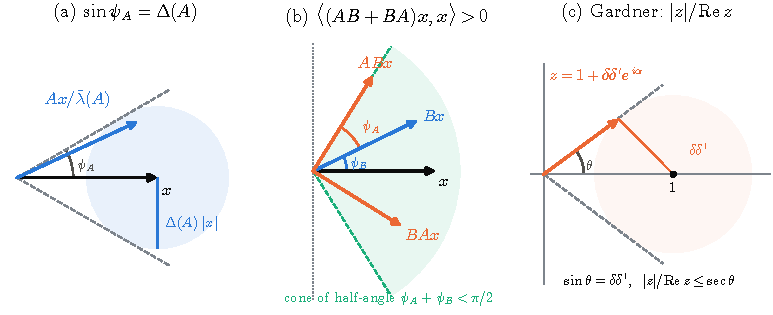
\includegraphics[width=\textwidth]{operator_angle.pdf}
\caption{(a) The angle of a positive operator: $Ax/\bar\lambda(A)$ lies in the ball of radius $\Delta(A)|x|$ about
$x$, so $\angle(x,Ax)\le\psi_A=\arcsin\Delta(A)$. (b) For a Jordan product the angles add; if $\psi_A+\psi_B<\pi/2$,
then $ABx$ and $BAx$ stay in a cone around $x$ that lies in the half-space of $x$, and $AB+BA>0$
(Theorem~\ref{thm:jordan}). (c) On a two-dimensional block, Gardner's quotient is $|z|/\Re z=\sec\arg z$ for a point $z$
on the circle of radius $\delta\delta'$ about $1$ (Remark~\ref{rem:geom}); the largest argument is $\arcsin(\delta\delta')$.}
\label{fig:angle}
\end{figure}

The theorem has a simple geometric meaning (Figure~\ref{fig:angle}). Krein~\cite{krein1969} and
Gustafson~\cite{gustafson1968} introduced the angle $\psi(A)$ of an operator, the largest angle between a vector $x$ and
its image $Ax$; for $A>0$, $\sin\psi(A)=\Delta(A)$, since $A$ divided by the midpoint $\bar\lambda(A)$ of its spectrum is
$1+E$ with $\|E\|=\Delta(A)$. If $|X|=vv^*$ has rank one ($\delta'=1$), Gardner's quotient is
$|\langle Wv,Uv\rangle|/\langle Wv,v\rangle\le\|Wv\|/\langle Wv,v\rangle=\sec\angle(v,Wv)\le\sec\psi(W)$, which is the
Kantorovich constant of $W$. For general $|X|$, the proof reduces to two-dimensional blocks on which $W$ and $|X|$ are,
up to scale, $1+\delta S$ and $1+\delta'S'$ with symmetries $S,S'$; there $\Tr(|X|W)$ and the trace norm
$\||X|W\|_1$ are $2\Re z$ and $2|z|$ for $z=1+\delta\delta'e^{i\alpha}$, where $e^{\pm i\alpha}$ are the eigenvalues of the
rotation $S'S$. Gardner's quotient is $\sec\arg z$, and the circle described by $z$ is seen from the origin under the
angle $\theta$ with $\sin\theta=\delta\delta'=\sin\psi(W)\sin\psi(|X|)$. The product of the contrasts is the radius of this
circle, and the constant of Theorem~A is $\sec\theta$.

\paragraph{Further results.} With the operators free, we determine the envelopes of 16 of the 25 inequalities exactly
and bound four others from below (Theorem~B in Section~\ref{sec:results}). The constants that appear are the
Kantorovich constant $\kappa=\sec\psi(W)$, the condition number of $W$ and the Specht ratio; the envelopes vanish at the
trace to the orders $\delta$, $\delta^2$, $\delta^4$ and $\delta^8$ (Figure~\ref{fig:ladder}). So the characterisations
differ greatly in sensitivity: two inequalities that are equivalent for traces may fail at different rates. Returning
to the unnormalised quantities of~\cite{abed2024}, we find the sharp bound of $|\Tr(XZ)|-\Tr(X|Z|)$ with both contrasts
prescribed and those of the two other trace functionals sampled there (Theorem~C), which answers the question
of~\cite{abed2024}. On a direct sum $\bigoplus_cM_{k_c}$ a functional is a trace when its density is central, however
different the scalars on the blocks, and accordingly only the contrast inside the blocks enters the envelopes
(Theorem~D).

The operators enter the inequalities through composites such as sums, congruences, Jordan products and commutators,
and Section~\ref{sec:composite} records how contrasts behave under these operations: the rapidities
$\operatorname{artanh}\Delta$ add under products and means (this is the triangle inequality of Hilbert's projective
metric), the angles $\arcsin\Delta$ add under Jordan products (Gustafson's criterion), and the commutator test
$\varphi(AB)=\varphi(BA)$ fails by exactly $2\Delta(W)\Delta(A)\Delta(B)$ in even dimension, after the natural
normalisation. These rules have a consequence for the inequalities themselves. The numerical search shows that
several characterisations are violated only by operators whose contrast is close to $1$. For subadditivity of the
square root, $\varphi((A+B)^{1/2})\le\varphi(A^{1/2})+\varphi(B^{1/2})$, we prove this: if $\Delta(A)=\Delta(B)\le2\sqrt2/3$,
then $A^{1/2}B^{1/2}+B^{1/2}A^{1/2}\ge0$ by Gustafson's criterion, hence $(A+B)^{1/2}\le A^{1/2}+B^{1/2}$ as operators, and
no positive functional can violate the inequality. For the power-mean inequality $\varphi(A^2)^{1/2}\le\varphi(A)$ we
find the envelope with both contrasts prescribed in closed form; it is never positive when $\Delta(A)\le\sqrt{(n-1)/n}$,
and this threshold is sharp (Section~\ref{sec:thresholds} and Figure~\ref{fig:square}).

\paragraph{What is new and what is classical.} The characterisation theorems are due to the cited authors. The
constants $\kappa$, $h$ and the Specht ratio, and the inequalities behind them (Kantorovich's inequality in the operator
form of Greub and Rheinboldt~\cite{greub1959}, Specht's reverse arithmetic--geometric mean
inequality~\cite{specht1960}), are classical, and so are several statements of Section~\ref{sec:composite}: the bounds
for congruences are the submultiplicativity of the condition number, the positivity criterion for Jordan products is
Gustafson's~\cite{gustafson1968}, and the norm bound for commutators of positive operators follows from Kittaneh's
inequality~\cite{kittaneh2008}. What we add is that the classical constants are the exact envelopes, the dependence on the
product of the contrasts in Theorem~A, the exact envelopes for pairs of projections (Theorem~\ref{thm:proj}), the
constructions that vanish to the orders $\delta^4$ and $\delta^8$, the sharp bounds of Theorem~C, the sharp trace
version of the commutator bound, and the threshold results of Section~\ref{sec:thresholds}. We know of no previous study
of the envelopes; the closest work is~\cite{abed2024}, which samples the unnormalised Gardner violation but defines no
envelope and proves no bound.

\paragraph{Numerical evidence.} For the inequalities without a closed form we computed the envelopes by constrained
optimisation over all operator variables. Every reported value is recomputed in 40-digit arithmetic at an exactly
admissible point, so it is a rigorous \emph{lower} bound for the supremum, not a certified value of it. Where the
envelope is known the search reproduces it to $10^{-7}$; elsewhere it supports the conjectured values of
Section~\ref{sec:open}. Two observations from the search guide the theory. First, the largest violation is usually found
at projections or at two-level operators $\ell+(1-\ell)P$; this is a theorem for the items to which the vertex principle
(Lemma~\ref{lem:vertex}) applies and an observation for the others, with exceptions in which the extremisers have three
eigenvalues. Second, random sampling, the method of~\cite{abed2024}, rarely comes close to the envelope: for
monotonicity and subadditivity fewer than one random sample in a thousand violates the inequality at all, so sampling
alone would suggest that these inequalities hold for every functional. The computations use the open-source library
described in the companion paper~\cite{lib}, which reproduces and extends the NumPy simulations of~\cite{abed2024};
part of the present results appears there as a use case.

\paragraph{Organisation.} Section~\ref{sec:related} reviews related work. Section~\ref{sec:setting} lists the
inequalities and collects the tools, and Section~\ref{sec:results} states Theorems B--D. Section~\ref{sec:gardner2}
proves Theorems~A and~C; Sections~\ref{sec:kant}, \ref{sec:linear}, \ref{sec:proj} and~\ref{sec:lower} prove Theorem~B,
and Section~\ref{sec:sectors} Theorem~D. Section~\ref{sec:composite} treats composite operators and the thresholds,
Section~\ref{sec:numerics} the numerical evidence, and Section~\ref{sec:open} lists conjectures and open problems.
Appendix~\ref{app:mc} shows the computed envelopes and random samples item by item.

\section{Related work}\label{sec:related}

\paragraph{Characterisations of the trace.} After Gardner~\cite{gardner1979}, traces on $M_n$ or among the positive
normal functionals on a von Neumann algebra were characterised by the triangle inequality for
$\varphi(|\cdot|)$~\cite{gardner1979,stolyarov2002}, by $|\varphi(A^k)|\le\varphi(|A|^k)$~\cite{petz1988}, by
monotonicity $0\le A\le B\Rightarrow\varphi(A^p)\le\varphi(B^p)$~\cite{bikchentaev2007mono,sano2006} and its weighted
forms~\cite{hoa2007,hoa2010}, by Young's inequality~\cite{bikchentaev2005young,cho2009}, by subadditivity of
$\varphi\circ f$ for concave $f$~\cite{tikhonov2005}, by the Peierls--Bogoliubov and Araki--Lieb--Thirring
inequalities~\cite{bikchentaev2011pb}, by the generalised Powers--St{\o}rmer inequality~\cite{hoa2013}, by inequalities
for determinants and power means~\cite{bikchentaev2020det}, by the spectral geometric mean~\cite{bikchentaev2026sgm}, by
inequalities for $|\varphi(A^2)|$~\cite{bikchentaev2026moslehian}, by metrics on projections~\cite{bikchentaev2019metric},
by subadditivity on the projection lattice~\cite[Theorem~4]{petz1988}, and by inequalities in which only projections
enter~\cite{bikchentaev2009rm,bikchentaev2010smj,bikchentaev2011mn,bikchentaev2019abed}. Bikchentaev and
Moslehian~\cite{bikchentaev2025survey} survey these results; the canonical trace on $M_n$ is characterised
in~\cite{moslehian2025jmaa,bikchentaev2020det}, and the dual problem, in which the functional is arbitrary and an
operator is to be recognised as central, is treated in~\cite{novikov2015}. All these results are qualitative.

\paragraph{Reverse inequalities.} Our upper bounds are reverse inequalities of Kantorovich type. Kantorovich's
inequality~\cite{kantorovich1948} and its operator form due to Greub and Rheinboldt~\cite{greub1959} bound
$\omega(W^2)\omega(1)$ by $\kappa^2\omega(W)^2$; the Mond--Pe\v{c}ari\'c method~\cite{furuta2005} produces such constants
systematically, and Specht's ratio~\cite{specht1960} is the sharp constant of the reverse arithmetic--geometric mean
inequality. The question here is different: not whether such a constant bounds the violation, but whether it is the
smallest one.

\paragraph{Operator angles.} Krein~\cite{krein1969} introduced the deviation of an operator and
Gustafson~\cite{gustafson1968} the equivalent angle $\psi(A)$, $\cos\psi(A)=\inf_{x\ne0}\Re\langle Ax,x\rangle/(\|Ax\|\|x\|)$,
the first antieigenvalue; for $0<m\le A\le M$ with $m,M$ in the spectrum, $\cos\psi(A)=2\sqrt{Mm}/(M+m)$ and
$\sin\psi(A)=(M-m)/(M+m)$~\cite{gustafsonrao1997,gustafson2012}. Thus the Michelson contrast of a positive operator is the
sine of its angle, and the Kantorovich constant is $\sec\psi(W)$. Gustafson used the angle to decide when products of
positive operators are accretive~\cite{gustafson1968}.

\paragraph{Jordan products.} The product $AB$ of positive operators is accretive exactly when the Jordan product
$AB+BA=2\Re(AB)$ is positive. Bounds for the eigenvalues of $AB+BA$ go back to Strang~\cite{strang1962} and
Nicholson~\cite{nicholson1979}; Alikakos and Bates~\cite{alikakos1984} bounded all eigenvalues and showed that Strang's
lower bound for the smallest one is best possible~\cite{alikakos1985}, and Conley, Pucci and Serrin~\cite{conley2005} gave
necessary and sufficient conditions for the positivity of the symmetrised product of two positive definite matrices.
Moslehian and Najafi~\cite[Theorem~2.1]{moslehian2011} proved that $AB+BA\ge0$ if and only if $f(A+B)\le f(A)+f(B)$ for
every non-negative operator monotone function $f$ on $[0,\infty)$. This links Jordan products to the subadditivity
inequalities that characterise traces~\cite{tikhonov2005}, and it is the background of Section~\ref{sec:thresholds}.

\paragraph{Commutators and Hilbert's metric.} Kittaneh~\cite{kittaneh2008} proved $\|XY-YX\|\le\|X\|\|Y\|$ when $X\ge0$,
which gives $\|AB-BA\|\le\frac12\|A\|\|B\|$ for positive $A,B$; versions for unitarily invariant norms
are in~\cite{kittaneh2007,bhatia2008}. On the cone of positive definite matrices, Thompson's
metric~\cite{thompson1963} is $d_T(A,B)=\|\log(A^{-1/2}BA^{-1/2})\|$ and Hilbert's projective
metric~\cite{bushell1973,lemmens2012} is $d_H(A,B)=\log\bigl(\lambda_{\max}/\lambda_{\min}\bigr)(A^{-1/2}BA^{-1/2})$. The
rapidity of a positive definite $A$ is
\[
  \operatorname{artanh}\Delta(A)=\tfrac12\log\frac{\lambda_{\max}(A)}{\lambda_{\min}(A)}=\tfrac12\,d_H(A,1)
  =\min_{t>0}d_T(A,t1),
\]
the Thompson distance of $A$ to the scalars; this is why rapidities behave additively under products
(Proposition~\ref{prop:rapid}).

\section{Setting and tools}\label{sec:setting}

\subsection{Functionals, contrast and envelopes}
Throughout, $\Tr$ is the usual trace on $M_n=M_n(\C)$, $|X|=(X^*X)^{1/2}$, $\|X\|_1=\Tr|X|$, $\Re X=\frac12(X+X^*)$,
and $\varphi=\varphi_W=\Tr(W\,\cdot\,)$ with $W\ge0$; $\varphi$ is a trace iff $W\in\C1$. We write $a\ge b$ for the
extreme eigenvalues of $W$, $e_1,e_2$ for corresponding unit eigenvectors, and $\delta=\Delta(W)$; unless stated
otherwise $W>0$, i.e.\ $\delta<1$. The quotient $(\cL-\cR)/\cN$ is invariant under $W\mapsto tW$, $t>0$, and the envelope
$V_n(\delta)$ is the supremum over all $W$ with $\Delta(W)=\delta$; for a fixed density we write $V(W)$. We call a
value of an envelope \emph{attained} if the supremum is a maximum and \emph{approached} otherwise. Variables called $P,Q,R$
are orthogonal projections, $A,B\ge0$ unless said otherwise, and $X,Y$ arbitrary; $P\wedge Q$ and $P\vee Q$ are the
projections onto $\mathrm{ran}\,P\cap\mathrm{ran}\,Q$ and onto $\mathrm{ran}\,P+\mathrm{ran}\,Q$.

\begin{table}[h]
\centering\small
\setlength{\tabcolsep}{3pt}
\begin{tabular}{rllll}
\toprule
 & inequality $\cL\le\cR$ & variables & $\cN$ & source\\
\midrule
1 & $|\varphi(X)|\le\varphi(|X|)$ & $X$ & $\cR$ & \cite{gardner1979}\\
2 & $\varphi(|X+Y|)\le\varphi(|X|)+\varphi(|Y|)$ & $X,Y$ & $\cR$ & \cite{gardner1979,stolyarov2002}\\
3 & $\varphi(A+A^*)\le2\varphi(|A^*|)$ & $A$ arbitrary & $\cR$ & \cite{bikchentaev2019abed}\\
4 & $|\varphi(A^2)|\le\varphi(A^*A)$ & $A$ arbitrary & $\cR$ & \cite[Thm.~1, $k=2$]{petz1988}, \cite{bikchentaev2026moslehian}\\
5 & $\varphi(|P-R|)\le\varphi(|P-Q|)+\varphi(|Q-R|)$ & $P,Q,R$ & $\cR$ & \cite{bikchentaev2019metric}\\
6 & $\varphi(A\natural B)\le\sqrt{\varphi(A)\varphi(B)}$ & $A,B>0$ & $\cR$ & \cite{bikchentaev2026sgm}\\
7 & $\varphi((B^{1/2}AB^{1/2})^2)\le\varphi(BA^2B)$ & $A,B$ & $\cR$ & \cite[Lemma~2, $r=2$, $p=1$]{bikchentaev2011pb}\\
8 & $\varphi(|AB^*|)\le\frac12\varphi(|A|^2)+\frac12\varphi(|B|^2)$ & $A,B$ arbitrary & $\cR$ & extension of \cite{bikchentaev2005young}\\
9 & $\varphi(PQ+QP)\le2\varphi(QPQ)$ & $P,Q$ & $\varphi(P)+\varphi(Q)$ & \cite{bikchentaev2019abed}\\
10 & $0\le A\le B\Rightarrow\varphi(A^2)\le\varphi(B^2)$ & $A\le B$ & $\cR$ & \cite{bikchentaev2007mono,sano2006}\\
11 & $(\det A)^{1/n}\le\frac1n\varphi(A)$, $\varphi(1)=n$ & $A$ & $(\det A)^{1/n}$ & \cite[Thm.~3(iii)]{bikchentaev2020det}\\
12 & $\varphi((A+B)^{1/2})\le\varphi(A^{1/2})+\varphi(B^{1/2})$ & $A,B$ & $\cR$ & \cite[Cor.~1]{tikhonov2005}\\
13 & $\varphi(A+B-|A-B|)\le2\varphi(A^{1/4}B^{1/2}A^{1/4})$ & $A,B$ & $\varphi(A+B)$ & \cite[Lemma~3.1]{hoa2013}\\
14 & $|\varphi(PQ)|\le\varphi(P)^{1/3}\varphi(Q)^{2/3}$ & $P,Q$ & $\cR$ & \cite[Thm.~2(i)]{bikchentaev2011mn}\\
15 & $\varphi(e^{P+Q})\le\varphi(e^{P/2}e^Qe^{P/2})$ & $P,Q$ & $\cR$ & \cite[Thm.~2(iv)]{bikchentaev2011mn}\\
16 & $\varphi(e^A)\exp\frac{\varphi(e^{A/2}Be^{A/2})}{\varphi(e^A)}\le\varphi(e^{A+B})$ & $A,B$ self-adj.\ & $\cR$ &
\cite[Lemma~1]{bikchentaev2011pb}\\
17 & $\varphi(PQP)\le\varphi(Q)$ & $P,Q$ & $\cR$ & \cite[Thm.~3.4(iv)]{bikchentaev2010smj}\\
18 & $\varphi(|P-Q|)\le\varphi(P+Q)$ & $P,Q$ & $\cR$ & \cite[Thm.~3.4(v)]{bikchentaev2010smj}\\
19 & $\varphi(P+Q)\le\varphi(1+P\wedge Q)$ & $P,Q$ & $\cR$ & \cite[Thm.~3.4(iii)]{bikchentaev2010smj}\\
20 & $\varphi(e^{QPQ})\le\varphi(e^P)$ & $P,Q$ & $\cR$ & \cite[Thm.~2(v)]{bikchentaev2011mn}\\
21 & $0\le\varphi(\Re PQ)$ & $P,Q$ & $\varphi(P)+\varphi(Q)$ & \cite[Thm.~2(vi)]{bikchentaev2011mn}\\
22 & $\varphi(\Re PQ)\le\varphi(|PQ|)$ & $P,Q$ & $\cR$ & \cite[Thm.~2(vii)]{bikchentaev2011mn}\\
23 & $\varphi(P\vee Q)\le\varphi(P)+\varphi(Q)$ & $P,Q$ & $\cR$ & \cite[Thm.~4]{petz1988}\\
24 & $\varphi(A^2)^{1/2}\le\varphi(A)$, $\varphi(1)=n$ & $A$ & $\cR$ & \cite[Thm.~3(vii)]{bikchentaev2020det}\\
25 & $0\le A\le B\Rightarrow\varphi(A^4)\le\varphi(AB^2A)$ & $A\le B$ & $\cR$ & \cite[Thms.~4, 5, $r=1$]{hoa2010}, \cite{hoa2007}\\
\bottomrule
\end{tabular}
\caption{The inequalities studied, with the normalisation $\cN$ of the violation $(\cL-\cR)/\cN$ and the source of the
characterisation. Projections are $P,Q,R$; positive operators $A,B$ unless stated otherwise. Remarks on the forms are
in Section~\ref{sec:forms}.}
\label{tab:items}
\end{table}

\subsection{Remarks on the forms}\label{sec:forms}
Several sources state families of inequalities; we use one member. In item~4, $|\varphi(A^k)|\le\varphi(|A|^k)$ for all
$A$ and one fixed $k\ge1$ characterises the trace on $M_n$~\cite[Theorem~1]{petz1988}; $k=1$ is Gardner's inequality.
Item~7 is the Araki--Lieb--Thirring inequality $\varphi((B^{1/2}AB^{1/2})^{rp})\le\varphi((B^{r/2}A^rB^{r/2})^p)$ with
$r=2$, $p=1$~\cite[Lemma~2]{bikchentaev2011pb}. The published form of item~8 is $\varphi(|AB|)\le\frac1p\varphi(A^p)+
\frac1q\varphi(B^q)$ for $A,B\ge0$~\cite{bikchentaev2005young}; we use $p=q=2$ and allow arbitrary $A,B$, in the form of
Ando's matrix Young inequality~\cite{ando1995}, and Proposition~\ref{prop:young} refers to this extension. Item~9 is the
member $p=1$ of the family $\varphi(PQ+QP)\le2\varphi((QPQ)^p)$, $p\in(0,1]$~\cite{bikchentaev2019abed}. Items 10 and 25
are the cases $r=0$ and $r=1$ of $\varphi(A^{2r+2})\le\varphi(A^rB^2A^r)$ for $0\le A\le B$, which characterises traces for
every fixed $r\ge0$~\cite[Lemma~1, Theorems~4,~5]{hoa2010}; on $M_n$ the case $r=0$ is
in~\cite{bikchentaev2007mono,sano2006} and $r>0$ in~\cite[Theorem~6]{hoa2007}. Items 11 and 24 characterise the
canonical trace among the positive functionals with $\varphi(1)=n$~\cite[Theorem~3]{bikchentaev2020det}; item~24 is (vii)
there with $p=2$, $q=1$ and needs $\varphi$ faithful. Item~12 is the case $f(t)=t^{1/2}$ of Tikhonov's
characterisation by $\varphi(f(A+B))\le\varphi(f(A))+\varphi(f(B))$ for concave $f$ with
$f(0)=0$~\cite[Corollary~1]{tikhonov2005}. Item~13 is the generalised Powers--St{\o}rmer inequality
$\varphi(A+B)-\varphi(|A-B|)\le2\varphi(f(A)^{1/2}g(B)f(A)^{1/2})$, $g(t)=t/f(t)$, with $f(t)=t^{1/2}$~\cite[Lemma~3.1,
Remark~4]{hoa2013}; with $\cN=\cR$ its envelope would be infinite (Remark~\ref{rem:13}), so we normalise by $\varphi(A+B)$.
Item~14 is Hölder's inequality for projections with the exponent $\alpha=3$; for $\alpha=2$ it holds for every positive
$\varphi$~\cite[remark after Theorem~2]{bikchentaev2011mn}. Item~16 is the Peierls--Bogoliubov inequality, stated
in~\cite{bikchentaev2011pb} for positive $H,K$; both sides scale by $e^c$ under $A\mapsto A+c$, $B\mapsto B+c$, so the
envelope over self-adjoint arguments is the same. Items 17--19 are~\cite[Theorem~3.4]{bikchentaev2010smj}, announced
in~\cite{bikchentaev2009rm}, and items 14, 15, 20--22 are~\cite[Theorem~2]{bikchentaev2011mn}.

\subsection{Tools}

\begin{lemma}[Kantorovich inequality~\cite{greub1959}]\label{lem:kant}
If $b\le W\le a$, $a\ge b>0$, then $\omega(W^2)\,\omega(1)\le\kappa^2\,\omega(W)^2$ for every positive functional
$\omega$, where $\kappa=(a+b)/(2\sqrt{ab})$.
\end{lemma}
\begin{proof}
$(a-W)(W-b)\ge0$ gives $\omega(W^2)\le(a+b)x-ab\,y$ with $x=\omega(W)$, $y=\omega(1)$, and $((a+b)x-aby)y\le\kappa^2x^2$
because the difference is $(\kappa x-\sqrt{ab}\,y)^2$.
\end{proof}

\begin{lemma}[Two projections; Halmos~\cite{halmos1969}]\label{lem:halmos}
For projections $P,Q$ on a finite-dimensional Hilbert space $H$, $H$ is the orthogonal sum of subspaces of dimension
$1$ or $2$ invariant under $P$ and $Q$. On each two-dimensional one there is an orthonormal basis $f,f'$ with $P=ff^*$
and $Q=qq^*$, $q=\cos\theta\,f+e^{i\chi}\sin\theta\,f'$, $0<\theta<\pi/2$.
\end{lemma}

The next lemma gives a general upper bound; it shows that no envelope of items 1--8 and 10 can exceed the order
$\delta$.

\begin{lemma}\label{lem:upper}
For items 1--8 and 10, $V(W)\le h-1$.
\end{lemma}
\begin{proof}
In each item $\cL\le a\cL_0$, where $\cL_0$ is the expression for the trace or the trace norm (e.g.\ $|\varphi(X)|\le a\|X\|_1$,
$\varphi(|X+Y|)\le a\Tr|X+Y|$, $|\varphi(A^2)|\le a\|A^2\|_1$), $\cL_0\le\cR_{\Tr}$ by the trace inequality (for item~4
$\|A^2\|_1\le\|A\|_2^2$; for item~7 the Araki--Lieb--Thirring inequality; for item~6, $A\natural B$ is unitarily similar to
$(A^{1/2}BA^{1/2})^{1/2}$, so $\Tr(A\natural B)=\|A^{1/2}B^{1/2}\|_1\le(\Tr A\Tr B)^{1/2}$), and $\cR\ge b\cR_{\Tr}$. Hence
$\cL/\cR\le a/b=h$. For item~8, $\varphi(|AB^*|)\le a\|A\|_2\|B\|_2\le\frac a2(\|A\|_2^2+\|B\|_2^2)$.
\end{proof}

\subsection{Contrasts of the operator variables}\label{sec:twocontrasts}

The envelope $V_n(\delta)$ lets the operator variables range over all operators. To see how the violation depends on
the operators themselves, we also prescribe their contrast. For a positive variable $A$ we use $\Delta(A)$, for an
arbitrary or self-adjoint variable $X$ the contrast $\Delta(|X|)$ of its modulus (for the Peierls--Bogoliubov
inequality, item~16, the variables are positive, as in~\cite{bikchentaev2011pb}), and we let every operator variable of
an item have the same contrast $\delta'\in[0,1]$:
\[
  V_n(\delta,\delta')=\sup\Bigl\{\frac{\cL-\cR}{\cN}:\ \Delta(W)=\delta,\ \text{every operator variable of contrast }\delta'\Bigr\}.
\]
Projections other than $0$ and $1$ have contrast $1$, so for items 5, 9, 14, 15 and 17--23 only $\delta'=1$ occurs, and
$V_n(\delta,1)\le V_n(\delta)$ with equality whenever the supremum over all operators is approached by singular ones.
A positive operator of contrast $\delta'$ whose spectrum has only two points is, up to a positive factor,
\[
  A=\ell'+(1-\ell')P,\qquad \ell'=\frac{1-\delta'}{1+\delta'},\qquad P\ \text{a projection},\ P\ne0,1;
\]
we call such operators \emph{two-level}. They are the affine images of projections, and as $\delta'\to1$ they become
scaled projections.

\begin{proposition}\label{prop:scalar}
If every operator variable is a positive multiple of the identity (for arbitrary and self-adjoint variables: if every
modulus is), then $\cL\le\cR$ in every item of Table~\ref{tab:items} and for every positive $\varphi$. Hence
$V_n(\delta,0)\le0$ for all items; and $V_n(0,\delta')\le0$, since for $\delta=0$ the functional is a multiple of the trace
(the canonical trace in items 11 and 24, where $\varphi(1)=n$).
\end{proposition}
\begin{proof}
Item by item, with $|X|=x$, $|Y|=y$ scalar and $X=xU$, $Y=yV$ with unitaries (symmetries for self-adjoint $X,Y$), and
$A=\alpha$, $B=\beta$ scalars: (1) $|\varphi(U)|\le\varphi(1)$; (2) $\varphi(|xU+yV|)\le\|xU+yV\|\varphi(1)\le(x+y)\varphi(1)$; (3) and (4)
as (1); (6) and (7) are equalities; (8) $|AB^*|=xy$ and $xy\le\frac12(x^2+y^2)$; (10) and (25) follow from $\alpha\le\beta$; (11) is an
equality for $\varphi(1)=n$; (12) $\sqrt{\alpha+\beta}\le\sqrt\alpha+\sqrt\beta$; (13) $\alpha+\beta-|\alpha-\beta|=2\min(\alpha,\beta)\le2\sqrt{\alpha\beta}$; (16) is an equality;
(24) $\varphi(\alpha^2)^{1/2}=\alpha\sqrt n\le\alpha n$.
\end{proof}

So a violation needs both contrasts: the functional must be far from a trace and the operators must be far from scalars.
The next lemma is the mechanism behind the two-level operators: whenever the violation depends convexly on the spectrum of a
variable, the extremal spectra have only two points.

\begin{lemma}[Vertex principle]\label{lem:vertex}
Fix all variables except the eigenvalues $\lambda\in[\ell',1]^n$ of one positive variable (its eigenbasis fixed), and let
$F(\lambda)$ and $\cN(\lambda)>0$ be the resulting values of $\cL-\cR$ and $\cN$. If $\lambda\mapsto F(\lambda)-c\cN(\lambda)$ is convex for
every $c\in\R$, then the supremum of $F/\cN$ over the spectra with $\max_i\lambda_i=1$ and $\min_i\lambda_i=\ell'$ equals its
supremum over the two-level spectra $\lambda\in\{\ell',1\}^n$ (both values occurring).
\end{lemma}
\begin{proof}
The admissible set is the union of the faces $\{\lambda_i=1,\ \lambda_j=\ell'\}$ of the cube, and the vertices of these faces are
the two-level spectra. If $F/\cN>c$ at an admissible point, then $F-c\cN>0$ there, and by convexity $F-c\cN>0$ at a vertex
of the same face, where therefore $F/\cN>c$.
\end{proof}

\noindent The hypothesis holds for Gardner's inequality ($F-c\cN=|\varphi(UT)|-(1+c)\varphi(T)$ for $X=UT$: the modulus of a
linear function minus a linear one), for item~3, for item~24 ($\varphi(A^2)^{1/2}=\|W^{1/2}A\|_2$ is a norm of a linear
function of $\lambda$) and for the unnormalised Gardner violation of Section~\ref{sec:gardner2}; for these items two-level
operators suffice. For the other items, whether they suffice is a question we examine numerically
(Section~\ref{sec:projsuffice}).

\section{Statement of the results}\label{sec:results}

Write $a\ge b>0$ for the extreme eigenvalues of $W$ and
\[
  h=\frac ab=\frac{1+\delta}{1-\delta},\qquad \kappa=\frac{a+b}{2\sqrt{ab}}=\frac1{\sqrt{1-\delta^2}}=\sec\psi,\qquad
  \psi=\arcsin\delta,
\]
the condition number, the Kantorovich constant and the angle of $W$. With the operator variables free, the envelopes are
as follows.

\begin{thmB}
\begin{enumerate}
\item[(a)] $V_n=\kappa-1$ for Gardner's inequality, the triangle inequalities for $\varphi(|\cdot|)$ on operators and on
projections, $\varphi(A+A^*)\le2\varphi(|A^*|)$, $|\varphi(A^2)|\le\varphi(A^*A)$, $\varphi(|P-Q|)\le\varphi(P+Q)$ and
$\varphi(\Re PQ)\le\varphi(|PQ|)$, in every dimension $n\ge2$ (Theorems~\ref{thm:kant} and~\ref{thm:proj}).
\item[(b)] $V_n=\kappa^2-1$ for $\varphi(PQP)\le\varphi(Q)$; $V_n=\frac12\tan^2(\psi/2)$ for $\varphi(\Re PQ)\ge0$;
$V_n=\delta/(1-\delta)$ for $\varphi(P\vee Q)\le\varphi(P)+\varphi(Q)$; $V_n=\delta$ for $\varphi(P+Q)\le\varphi(1+P\wedge Q)$
($n$ even); and $V_n$ is the maximum of an explicit function of one variable, $\frac{(e-1)^2}{e(e+1)}\delta^2+O(\delta^3)$, for
$\varphi(e^{QPQ})\le\varphi(e^P)$ ($n$ even) (Theorem~\ref{thm:proj}).
\item[(c)] $V_n=h-1$ for the extension of Young's inequality to arbitrary operators; $V_2=s/(1+s)$, $s=\sin(\psi/2)$, for
$\varphi(PQ+QP)\le2\varphi(QPQ)$; for the inequalities that characterise the \emph{canonical} trace, $V_2=1-\sqrt{1-\delta^2}$
for the inequality $(\det A)^{1/n}\le\frac1n\varphi(A)$, increasing with $n$ to $1-1/S(h)$ with the Specht ratio $S$,
and $V_n=\sqrt{(\ell+n-1)/(n\ell)}-1$, $\ell=1/h$, for $\varphi(A^2)^{1/2}\le\varphi(A)$ (Section~\ref{sec:linear}).
\item[(d)] $V_n\ge\kappa-1$ for the spectral geometric mean inequality, $V_n\ge\kappa^2-1$ for the Araki--Lieb--Thirring
inequality, $V_n\ge\delta^4/16+O(\delta^5)$ for monotonicity and $V_n\ge\delta^8/4096\,(1+O(\delta^2))$ for its weighted form
with $r=1$; and $V_n\le h-1$ for items 1--8 and~10 (Section~\ref{sec:lower} and Lemma~\ref{lem:upper}).
\end{enumerate}
\end{thmB}

\begin{figure}[t]
\centering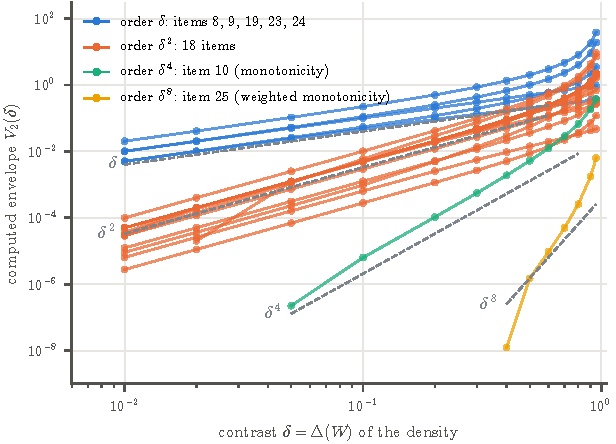
\includegraphics[width=0.72\textwidth]{ladder_of_orders.pdf}
\caption{The ladder of orders: the computed envelopes $V_2(\delta)$ of all 25 items (certified lower bounds for the
suprema, Section~\ref{sec:numerics}) on logarithmic axes, coloured by the order of vanishing at the trace, with guide
lines of slopes $1$, $2$, $4$ and~$8$. Item~25 is resolved by the search only for $\delta\ge0.4$.}
\label{fig:ladder}
\end{figure}

The envelopes thus vanish at the trace to different orders, $\delta$, $\delta^2$, $\delta^4$ and $\delta^8$
(Figure~\ref{fig:ladder} and Table~\ref{tab:classes}), and two inequalities that are equivalent for traces may fail at
different rates. For instance, $\varphi(P\vee Q)+\varphi(P\wedge Q)=\varphi(P)+\varphi(Q)$ for every trace, yet the lattice
subadditivity fails as $\delta/(1-\delta)$, while $\varphi(|P-Q|)\le\varphi(P+Q)$, with the same right-hand side, fails only as
$\kappa-1\sim\delta^2/2$. The orders refer to the normalisations $\cN$ of Table~\ref{tab:items}; a normalisation that
vanishes at the extremisers can change them (Remark~\ref{rem:13}).

The third result returns to the unnormalised quantity of~\cite{abed2024}, in which both operators are normalised to
norm one and both contrasts are prescribed. Let $\nu=\sum_c\lfloor k_c/2\rfloor$ be the largest number of mutually
orthogonal two-dimensional subspaces that fit into the blocks of $\M$.

\begin{thmC}
Let $\M=\bigoplus_{c=1}^CM_{k_c}(\mathbb K)$, $\mathbb K\in\{\R,\C\}$, with $\nu\ge1$. For $X\ge0$ and $Z$ in $\M$ with
$\|X\|=\|Z\|=1$, $\Delta(X)=\delta<1$ and $\Delta(|Z|)=\delta'$,
\[
  \sup\bigl(|\Tr(XZ)|-\Tr(X|Z|)\bigr)=\frac{\nu\,\delta^2\delta'^2}{(1+\delta)(1+\delta')},
\]
and the supremum is attained (Theorem~\ref{thm:gardner2}). The two other functionals of~\cite{abed2024},
$\Tr|XY|-\Tr(|X||Y|)$ and $\Tr(Y|X|Y)-\Tr|YXY|$, have the sharp bounds of Proposition~\ref{prop:exp2} and
Theorem~\ref{thm:exp3}.
\end{thmC}

On a finite-dimensional von Neumann algebra $\M=\bigoplus_{c=1}^CM_{k_c}$ a positive functional $\varphi_W$ is a trace if
and only if $W$ is central, i.e.\ scalar on every block, however different the scalars are. The violation therefore
cannot depend on the global contrast of $W$:

\begin{thmD}
Let $W=\bigoplus_cW_c>0$ in $\M$. For every inequality of Table~\ref{tab:items} except 11, 16 and 24, the largest
normalised violation for $\varphi_W$ on $\M$ is at most the largest one for $\varphi_{W_c}$ on the blocks $M_{k_c}$, with
equality for items 1--10, 12--14, 17, 18, 21--23 and~25. A density that varies only between the blocks violates none of the
inequalities except 11 and~24, which characterise the canonical trace (Theorem~\ref{thm:sectors}).
\end{thmD}

\section{The Kantorovich class}\label{sec:kant}

\begin{theorem}\label{thm:kant}
Let $W>0$ in $M_n$, $n\ge2$, and $\varphi=\varphi_W$. For all $X,Y,A$ and all projections $P,Q,R$,
\begin{gather*}
|\varphi(X)|\le\kappa\,\varphi(|X|),\qquad \varphi(A+A^*)\le2\kappa\,\varphi(|A^*|),\qquad |\varphi(A^2)|\le\kappa\,\varphi(A^*A),\\
\varphi(|X+Y|)\le\kappa\bigl(\varphi(|X|)+\varphi(|Y|)\bigr),\qquad
\varphi(|P-R|)\le\kappa\bigl(\varphi(|P-Q|)+\varphi(|Q-R|)\bigr).
\end{gather*}
All five constants are attained. Hence $V_n=\kappa-1$ for items 1--5 in every dimension $n\ge2$.
\end{theorem}
\begin{proof}
Let $X=U|X|$ be a polar decomposition and $T=|X|$. Then $\varphi(X)=\Tr(WUT)=\Tr\bigl((WT^{1/2})^*UT^{1/2}\bigr)$, so for every contraction $U$
\[
  |\varphi(X)|^2\le\Tr(W^2T)\,\Tr T\le\kappa^2(\Tr WT)^2
\]
by the Cauchy--Schwarz inequality and Lemma~\ref{lem:kant} for $\omega=\Tr(T\,\cdot\,)$. The second inequality follows in the same way from
$\varphi(A+A^*)=2\Re\varphi(|A^*|V)$, where $A=|A^*|V$ is a polar decomposition. For the fourth, write $X+Y=S|X+Y|$; then $\varphi(|X+Y|)=\varphi(S^*X)+\varphi(S^*Y)$, and each term
is bounded as above with the contraction $S^*U_X$ or $S^*U_Y$ in place of $U$. The fifth is the fourth with $X=P-Q$,
$Y=Q-R$. For the third, put $X=AW^{1/2}$ in an eigenbasis of $W$ with eigenvalues $w_i$. Then $\varphi(A^*A)=\sum_{ij}|X_{ij}|^2$ and
\[
  \varphi(A^2)=\sum_iX_{ii}^2+\sum_{i<j}X_{ij}X_{ji}\frac{w_i+w_j}{\sqrt{w_iw_j}},\qquad\frac{w_i+w_j}{\sqrt{w_iw_j}}\le2\kappa,
\]
so $|\varphi(A^2)|\le\sum_i|X_{ii}|^2+\kappa\sum_{i<j}(|X_{ij}|^2+|X_{ji}|^2)\le\kappa\varphi(A^*A)$.

Equality, with $e_1,e_2$ eigenvectors of $W$ for $a,b$: in the first two inequalities for $T=vv^*$ with
$|\langle e_1,v\rangle|^2=\frac b{a+b}$, $|\langle e_2,v\rangle|^2=\frac a{a+b}$ and $Uv=Wv/\|Wv\|$ (equality in
Cauchy--Schwarz and in Lemma~\ref{lem:kant}); in the third for $A=\sqrt a\,e_1e_2^*+\sqrt b\,e_2e_1^*$; in the fourth for
$X=uu^*$, $Y=-u'u'^*$ with $u,u'=\sin t\,e_1\pm\cos t\,e_2$ and $\tan t=\sqrt{b/a}$; in the fifth for $P=uu^*$, $Q=0$,
$R=u'u'^*$.
\end{proof}

\begin{remark}
For a fixed density, $\sup_X|\varphi(X)|/\varphi(|X|)=\kappa(W)$ exactly. In particular the normalised violation of
Gardner's inequality depends on $W$ only through its extreme eigenvalues, not on the dimension or on the rest of the
spectrum.
\end{remark}

\section{Gardner's inequality with two contrasts}\label{sec:gardner2}

For Gardner's inequality both contrasts can be prescribed and the envelope found exactly. It depends on the two contrasts
only through their product.

\begin{theorem}\label{thm:gardnerD}
Let $W>0$ and $X$ be in $M_n$, $n\ge2$, with $\Delta(W)=\delta$ and $\Delta(|X|)=\delta'$, $\delta,\delta'\in[0,1]$,
$\delta\delta'<1$. Then
\[
  |\varphi_W(X)|\le\frac{1}{\sqrt{1-\delta^2\delta'^2}}\,\varphi_W(|X|),
\]
and for even $n$ the constant is attained: $V_n(\delta,\delta')=\kappa(\delta\delta')-1=(1-\delta^2\delta'^2)^{-1/2}-1$
for Gardner's inequality. For odd $n=2k+1$,
\[
  V_n(\delta,\delta')=\max_{0\le\gamma\le1}\frac{k\sqrt{S^2+\gamma pq}+\ell\ell'}{k(S+\gamma p)+\ell\ell'}-1,\qquad
  S=\ell+\ell',\ q=(1+\ell)(1+\ell'),\ p=(1-\ell)(1-\ell'),
\]
with $\ell=\frac{1-\delta}{1+\delta}$, $\ell'=\frac{1-\delta'}{1+\delta'}$; it is smaller than $\kappa(\delta\delta')-1$ for
$\delta'<1$ and tends to it as $n\to\infty$. For $\delta'=1$ both give Theorem~\ref{thm:kant}. The upper bound
$\kappa(\delta\delta')$ holds also for items 2 and~3, with the contrasts of $|X|,|Y|$ and of $|A^*|$.
\end{theorem}
\begin{proof}
Write $X=UT$ with $T=|X|$. The supremum of $|\Tr(WUT)|=|\Tr(U\,TW)|$ over unitaries $U$ is $\|TW\|_1$, so we must bound
$\|TW\|_1/\Tr(TW)$. For fixed eigenbases, $\|TW\|_1-c\Tr(TW)$ is a convex function of the eigenvalues of $T$ (a norm of a
linear function minus a linear one), and likewise of the eigenvalues of $W$. By Lemma~\ref{lem:vertex}, applied to $T$ and
then to $W$, we may assume $W=a(\ell+(1-\ell)P)$ and $T=t(\ell'+(1-\ell')Q)$ with projections $P,Q$ and $\ell=\frac{1-\delta}{1+\delta}$,
$\ell'=\frac{1-\delta'}{1+\delta'}$. By Lemma~\ref{lem:halmos}, $\C^n$ splits into subspaces of dimension $1$ or $2$ invariant
under $P$ and $Q$, hence under $W$ and $T$, and $\|TW\|_1$ and $\Tr(TW)$ are sums over them. On a one-dimensional summand the
two contributions are equal. On a two-dimensional one, $W$ and $T$ have the eigenvalues $x_1,x_2$ and $y_1,y_2$, namely
$a,a\ell$ and $t,t\ell'$; with $S=x_1y_2+x_2y_1$, $q=(x_1+x_2)(y_1+y_2)$, $p=(x_1-x_2)(y_1-y_2)$ and $\gamma$ the squared overlap
of the leading eigenvectors, the proof of Proposition~\ref{prop:k2} gives $\|TW\|_1^2=S^2+\gamma pq$ and $\Tr(TW)=S+\gamma p$.
The function $\gamma\mapsto(S^2+\gamma pq)/(S+\gamma p)^2$ is maximal at $\gamma=S/q\in[0,1]$, with the value
\[
  \frac{q^2}{4S(S+p)}=\frac{(x_1+x_2)^2(y_1+y_2)^2}{4(x_1y_2+x_2y_1)(x_1y_1+x_2y_2)}=\frac1{1-\delta^2\delta'^2},
\]
the last step by inserting $x_2/x_1=\ell$, $y_2/y_1=\ell'$. A quotient of sums is at most the largest quotient of the
summands. Equality for even $n$: $n/2$ copies of the $2\times2$ configuration $W=\mathrm{diag}(1,\ell)$, $T$ with the
eigenvalues $1,\ell'$ at $\gamma=S/q$, and $U$ the adjoint polar factor of $TW$. For odd $n$ at least one summand is
one-dimensional and contributes the same amount $\mu\ge\ell\ell'$ (normalising the largest eigenvalues of $W$ and $T$
to $1$) to $\|TW\|_1$ and to $\Tr(TW)$; the quotient $(\sum_js_j+\mu)/(\sum_jt_j+\mu)$, where $s_j\ge t_j$ are the
contributions of at most $k$ two-dimensional summands, is largest for $k$ summands and $\mu=\ell\ell'$, and, by the argument
of Lemma~\ref{lem:vertex} applied to $s-ct$, for the same $\gamma$ in every summand, which gives the stated maximum; it is attained by
$W=\mathrm{diag}(1,\ell)^{\oplus k}\oplus\ell$ and $T$ correspondingly. Items 2 and~3 reduce to the first inequality as in
the proof of Theorem~\ref{thm:kant}.
\end{proof}

\noindent Thus the normalised violation of Gardner's inequality is $\frac12\delta^2\delta'^2+O(\delta^4\delta'^4)$: it
vanishes to second order in each contrast and is symmetric in the density and the operator. For a Gibbs state at inverse
temperature $\beta$ and an operator $|X|=e^{-\beta' K}$, the constant is $(1-\tanh^2(\beta\Delta E/2)\tanh^2(\beta'\Delta
E'/2))^{-1/2}$, where $\Delta E$ and $\Delta E'$ are the spectral spreads of $H$ and $K$. The two-dimensional computation in
the proof has a transparent form, which explains the dependence on the product.

\begin{remark}[Geometric form]\label{rem:geom}
On $\C^2$ let $W=w(1+\delta S)$ and $T=t(1+\delta'S')$ with $w,t>0$ and symmetries $S,S'$ of trace zero. The unitary $S'S$ has
determinant $1$, hence eigenvalues $e^{\pm i\alpha}$, and $\Tr(SS')=\Tr(S'S)=2\cos\alpha$. Then
\[
  \Tr(TW)=2wt\,\Re z,\qquad \|TW\|_1=2wt\,|z|,\qquad z=1+\delta\delta'e^{i\alpha}.
\]
The first identity follows from $\Tr(TW)=wt\Tr(1+\delta S+\delta'S'+\delta\delta'S'S)$. For the second, $\|M\|_1^2=\Tr(M^*M)+
2|\det M|$ for $2\times2$ matrices, and $\Tr(W^2T^2)=w^2t^2\Tr\bigl((1+\delta^2+2\delta S)(1+\delta'^2+2\delta'S')\bigr)=
2w^2t^2\bigl((1+\delta^2)(1+\delta'^2)+4\delta\delta'\cos\alpha\bigr)$ and $|\det TW|=w^2t^2(1-\delta^2)(1-\delta'^2)$ add up to
$4w^2t^2|z|^2$. So Gardner's quotient $\sup_U|\Tr(WUT)|/\Tr(WT)$ equals $|z|/\Re z=\sec\arg z$. As the relative position of
$W$ and $T$ varies, $z$ runs over the circle of radius $\delta\delta'$ about $1$, whose points have $|\arg z|\le\theta$,
$\sin\theta=\delta\delta'$, with equality for $\cos\alpha=-\delta\delta'$ (Figure~\ref{fig:angle}(c)). This gives the
$2\times2$ case of Theorem~\ref{thm:gardnerD}, with the constant $\sec\theta=(1-\delta^2\delta'^2)^{-1/2}$. Since
$\delta=\sin\psi(W)$ and $\delta'=\sin\psi(T)$, the angle $\theta$ is determined by $\sin\theta=\sin\psi(W)\sin\psi(T)$.
\end{remark}

The unnormalised violation studied in~\cite{abed2024} behaves in the same way (Theorem~\ref{thm:gardner2} below).

In~\cite[Sect.~5]{abed2024} the violation of Gardner's inequality was studied without normalisation: for $X\ge0$ with
$\|X\|=1$ (the density) and $Z$ with $\|Z\|=1$, the quantity
\[
  z(X,Z)=|\Tr(XZ)|-\Tr(X|Z|)
\]
was sampled against $\Delta(X)$ and $\Delta(|Z|)$. Writing $Z=U|Z|$ with a unitary (orthogonal, in the real case) $U$,
$z=|\Tr(XUY)|-\Tr(XY)$ with $Y=|Z|\ge0$, and $\sup_Uz=\|YX\|_1-\Tr(XY)$ by the duality of the trace norm, the supremum being
attained at the polar unitary of $YX$, which is real if $X,Y$ are. We first solve the $2\times2$ case.

\begin{proposition}\label{prop:k2}
Let $X,Y\ge0$ in $M_2(\C)$ have eigenvalues $x_1\ge x_2\ge0$ and $y_1\ge y_2\ge0$, $x_1,y_1>0$. For every unitary $U$,
\[
  |\Tr(XUY)|-\Tr(XY)\ \le\ \frac{(x_1-x_2)^2(y_1-y_2)^2}{4(x_1+x_2)(y_1+y_2)} .
\]
Let $S=x_1y_2+x_2y_1$, $q=(x_1+x_2)(y_1+y_2)$, and $\gamma=|\langle e_1,f_1\rangle|^2$ for unit eigenvectors $e_1$ of $X$ for
$x_1$ and $f_1$ of $Y$ for $y_1$. If $x_1>x_2$ and $y_1>y_2$, the bound is attained iff $|\Tr(XUY)|=\|YX\|_1$ and
$\gamma=\frac14+\frac S{2q}$; it is attained by real $X,Y,U$.
\end{proposition}
\begin{proof}
Let $p=(x_1-x_2)(y_1-y_2)$, so that $q-2S=p$. First, $|\Tr(XUY)|=|\Tr(YXU)|\le\|YX\|_1$. Expanding in the eigenbases,
$\Tr(XY)=\sum_{ij}x_iy_j|\langle e_i,f_j\rangle|^2=S+\gamma p$, since the matrix $(|\langle e_i,f_j\rangle|^2)$ is doubly
stochastic. The singular values of $YX$ satisfy $s_1^2+s_2^2=\Tr(X^2Y^2)$ and $s_1s_2=|\det YX|=x_1x_2y_1y_2$, so
$\|YX\|_1^2=\Tr(X^2Y^2)+2x_1x_2y_1y_2=S^2+\gamma pq$. With $\sqrt r\le r/q+q/4$ (equality iff $\sqrt r=q/2$),
\[
  \|YX\|_1-\Tr(XY)\le\frac{S^2+\gamma pq}q+\frac q4-S-\gamma p=\frac{(q/2-S)^2}q=\frac{p^2}{4q},
\]
with equality iff $\gamma pq=q^2/4-S^2=\frac p2(\frac q2+S)$. Every $\gamma\in[0,1]$ is realised by a real rotation, and the
polar unitary of a real $YX$ is real.
\end{proof}

\begin{theorem}\label{thm:gardner2}
Let $\M=\bigoplus_{c=1}^CM_{k_c}(\mathbb K)$, $\mathbb K\in\{\R,\C\}$, and $\nu=\sum_c\lfloor k_c/2\rfloor\ge1$. For $X\ge0$ and
$Y\ge0$ in $\M$ with $\|X\|=\|Y\|=1$, $\Delta(X)=\delta\in[0,1)$ and $\Delta(Y)=\delta'\in[0,1]$, and every unitary
(orthogonal) $U\in\M$,
\[
  |\Tr(XUY)|-\Tr(XY)\le\frac{\nu\,\delta^2\delta'^2}{(1+\delta)(1+\delta')},
\]
and the bound is attained. Equivalently, $\sup\{|\Tr(XZ)|-\Tr(X|Z|):\|X\|=\|Z\|=1,\ \Delta(X)=\delta,\ \Delta(|Z|)=\delta'\}$
has this value.
\end{theorem}
\begin{proof}
Let $\ell=(1-\delta)/(1+\delta)$ and $\ell'=(1-\delta')/(1+\delta')$ be the smallest eigenvalues. It suffices to prove the
bound in the complex algebra, since the maximisers below are real. By the remark above, $\sup_Uz=F(X,Y):=\|YX\|_1-\Tr(XY)$,
and the polar unitary lies in $\M$. For a fixed eigenbasis of $X$, $F$ is a convex function of the eigenvalues of $X$ (a
norm of a linear function of them minus a linear function). The admissible eigenvalues form the union of the faces
$\{x_i=1,\ x_j=\ell\}$ of the cube $[\ell,1]^K$, $K=\sum_ck_c$, and a convex function on a face attains its maximum at a vertex; so
$F(X,Y)\le F(X',Y)$ for some $X'=\ell+(1-\ell)P$ with a projection $P\in\M$, $P\ne0,1$, and likewise $F(X',Y)\le F(X',Y')$
with $Y'=\ell'+(1-\ell')Q$. By Lemma~\ref{lem:halmos}, applied in every block, $X'$ and $Y'$ are direct sums over subspaces of
dimension $1$ or $2$, and so are $\|Y'X'\|_1$ and $\Tr(X'Y')$. One-dimensional summands contribute $0$. On a
two-dimensional one, $X'=\mathrm{diag}(1,\ell)$ and $Y'$ has the eigenvalues $1,\ell'$, so by Proposition~\ref{prop:k2} it
contributes at most $(1-\ell)^2(1-\ell')^2/(4(1+\ell)(1+\ell'))=\delta^2\delta'^2/((1+\delta)(1+\delta'))$. A block of size
$k_c$ holds at most $\lfloor k_c/2\rfloor$ two-dimensional summands. Equality: $\nu$ blocks $\mathrm{diag}(1,\ell)$ and
$Y$ with spectrum $\{1,\ell'\}$ at the angle of Proposition~\ref{prop:k2}, $X=Y=1$ on the remaining one-dimensional blocks,
and the polar unitary, which makes all block traces positive.
\end{proof}

\begin{figure}[t]
\centering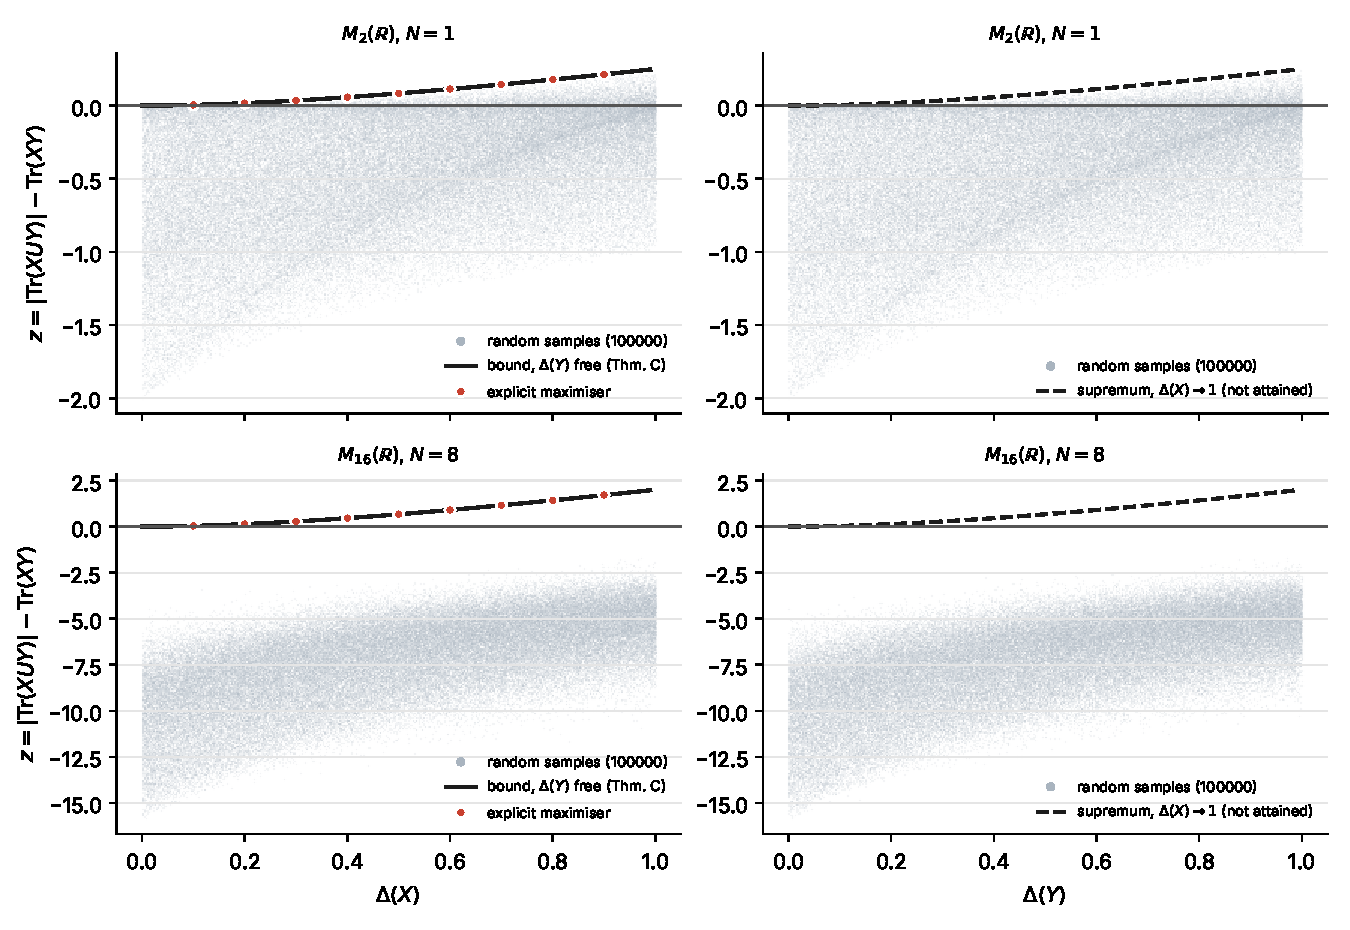
\includegraphics[width=\textwidth]{gardner_contrasts.pdf}
\caption{The unnormalised Gardner violation $z=|\Tr(XUY)|-\Tr(XY)$ for $\|X\|=\|Y\|=1$ in $M_2(\R)$ (top, $\nu=1$) and
$M_{16}(\R)$ (bottom, $\nu=8$; the panels write $N$ for $\nu$), against $\Delta(X)$ (left) and $\Delta(Y)$ (right). Grey: $100000$ random samples with
Haar-orthogonal eigenbases and $U$ and uniformly drawn contrasts, as in~\cite[Fig.~1]{abed2024}. Solid: the bound of
Theorem~\ref{thm:gardner2} with $\Delta(Y)$ free, $\nu\delta^2/(2(1+\delta))$; dots: $z$ at the explicit maximisers of its
proof, which agree with it to $10^{-15}$. Dashed: the supremum along $\Delta(Y)$, approached as $\Delta(X)\to1$. In
$M_{16}$ no sample violates Gardner's inequality ($z>0$), although violations up to almost $2$ exist: the maximisers,
two-level spectra on aligned pairs of eigenvectors, form a set of negligible Haar measure. Computed with plain NumPy by
\texttt{scripts/\allowbreak trace\_\allowbreak envelopes\_\allowbreak figures.py}.}
\label{fig:gardner1d}
\end{figure}

\begin{figure}[t]
\centering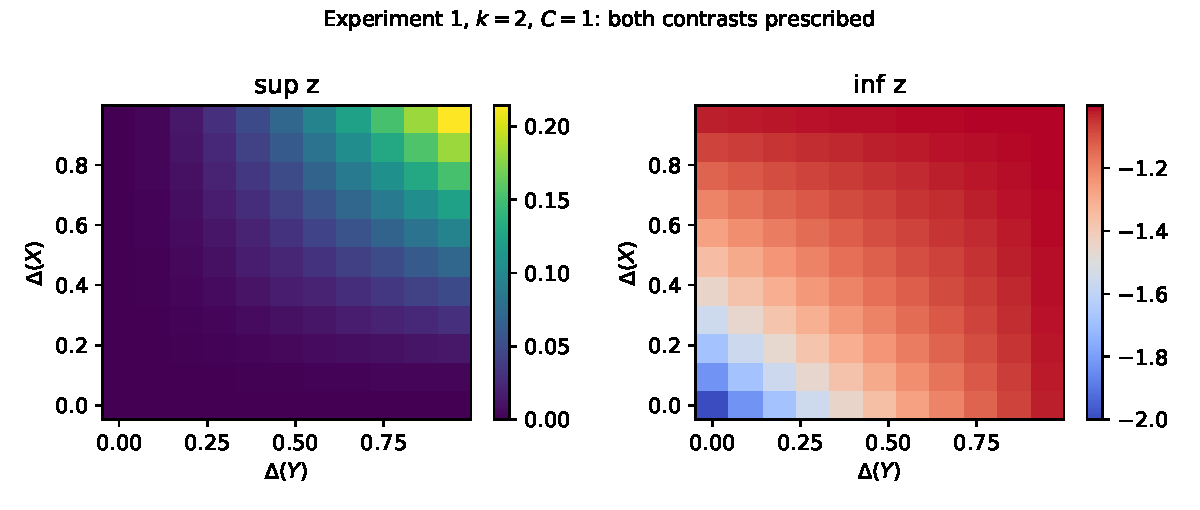
\includegraphics[width=0.8\textwidth]{bounds2d_exp1_k2_C1.pdf}
\caption{$M_2(\R)$, both contrasts prescribed: the supremum (left) and infimum (right) of
$z=|\Tr(XUY)|-\Tr(XY)$ found by constrained optimisation on a grid of $\Delta(Y)$ (horizontal) and $\Delta(X)$
(vertical). The left panel agrees with $\delta^2\delta'^2/((1+\delta)(1+\delta'))$ (Theorem~\ref{thm:gardner2}) to
$5\times10^{-10}$ at every grid point: a violation needs both operators to be far from scalar.}
\label{fig:gardner2d}
\end{figure}

\begin{remark}
(i) With the contrast of $|Z|$ free, the supremum $\nu\delta^2/(2(1+\delta))$ is reached at $\delta'=1$, i.e.\ for singular $Z$.
(ii) The bound is additive over the blocks: it counts the mutually orthogonal two-dimensional subspaces that fit into the
blocks, and it does not depend on the sizes of the blocks otherwise. (iii) The normalised version is
Theorem~\ref{thm:kant}: $\sup_Z|\Tr(XZ)|/\Tr(X|Z|)=\kappa(X)$, attained by a rank-one $|Z|$, i.e.\ at $\Delta(|Z|)=1$.
The unnormalised supremum vanishes to fourth order at $\delta=\delta'=0$ because the violation needs both operators to be
far from scalar. (iv) Figures~\ref{fig:gardner1d} and~\ref{fig:gardner2d} compare the bound with random sampling and with
numerical optimisation. Sampling, the method of~\cite{abed2024}, stays far below the bound as soon as the blocks are
larger than $2\times2$, while the optimisation over both contrasts reproduces it.
\end{remark}

\subsection{The other two functionals of~\cite{abed2024}}\label{sec:exp23}

Besides Gardner's inequality, \cite[Sect.~5]{abed2024} sampled two further unnormalised trace functionals,
\[
  z_2=\Tr|XY|-\Tr(|X|\,|Y|),\qquad z_3=\Tr(Y|X|Y)-\Tr|YXY|\quad(X=X^*,\ Y\ge0),
\]
with $|X|$ and $|Y|$ normalised to $\lambda_{\max}=1$ and their contrasts as parameters. Both are determined here in
$\M=\bigoplus_cM_{k_c}$, with $\nu=\sum_c\lfloor k_c/2\rfloor$ and $\ell=\frac{1-\delta}{1+\delta}$, $\ell'=\frac{1-\delta'}{1+\delta'}$
as before; note $1-\ell=\frac{2\delta}{1+\delta}$.

\begin{proposition}\label{prop:exp2}
Let $X=UX_0$, $Y=VY_0$ with $X_0,Y_0\ge0$ and unitaries $U,V\in\M$, so that $|X|=X_0$, $|Y|=Y_0$ and
$z_2=\|X_0VY_0\|_1-\Tr(X_0Y_0)$. For given spectra,
\[
  \sup z_2=-\inf z_2=\sum_c\sum_ix_{c,i}^\downarrow\bigl(y_{c,i}^\downarrow-y_{c,i}^\uparrow\bigr),
\]
with $x_{c,i}^\downarrow$ the eigenvalues of $X_{0,c}$ in decreasing order and $y_{c,i}^\downarrow$, $y_{c,i}^\uparrow$ those of
$Y_{0,c}$ in decreasing and increasing order. With $\Delta(|X|)=\delta$ and $\Delta(|Y|)=\delta'$ prescribed,
$\sup z_2=-\inf z_2=\nu(1-\ell)(1-\ell')=\frac{4\nu\delta\delta'}{(1+\delta)(1+\delta')}$, attained by two-level spectra.
\end{proposition}
\begin{proof}
$V$ and the eigenbases act sector by sector, and von Neumann's trace inequality $\|AB\|_1\le\sum_is_i(A)s_i(B)$, its lower
counterpart $\|AB\|_1\ge\sum_is_i(A)s_{k+1-i}(B)$ and the rearrangement inequality for $\Tr(X_0Y_0)$ give the first
formula; both extremes are attained by aligning or reversing the eigenbases. Pairing $i$ with $k+1-i$,
$\sum_ix_{c,i}^\downarrow(y_{c,i}^\downarrow-y_{c,i}^\uparrow)=\sum_{i\le k/2}(x_{c,i}^\downarrow-x_{c,k+1-i}^\downarrow)
(y_{c,i}^\downarrow-y_{c,k+1-i}^\downarrow)\le\lfloor k/2\rfloor(1-\ell)(1-\ell')$, with equality for two-level spectra.
\end{proof}

\noindent So $z_2$ is linear in each contrast, unlike Gardner's violation, which is quadratic in each. The third
functional is never negative:

\begin{proposition}\label{prop:exp3eq}
For $X=X^*$ and $Y\ge0$, $\Tr|YXY|\le\Tr(Y|X|Y)$, with equality if and only if $YX_+Y^2X_-Y=0$, in particular if $Y$
commutes with $X$.
\end{proposition}
\begin{proof}
With $X=X_+-X_-$ and $|X|=X_++X_-$, the triangle inequality for the trace norm gives
$\|YX_+Y-YX_-Y\|_1\le\Tr(YX_+Y)+\Tr(YX_-Y)$. For positive $A,B$, $\|A-B\|_1=\Tr A+\Tr B$ if and only if $AB=0$: with $P$
the projection onto the positive part of $A-B$, $\|A-B\|_1=\Tr A+\Tr B-2\Tr((1-P)A)-2\Tr(PB)$, and equality forces
$(1-P)A=0=PB$, so $AB=AP(1-P)B=0$; conversely, if $AB=0$ the supports are orthogonal and $|A-B|=A+B$. Apply this to
$A=YX_+Y$, $B=YX_-Y$. If $XY=YX$, then $YX_+Y^2X_-Y=Y^4X_+X_-=0$.
\end{proof}

\begin{proposition}\label{prop:k2b}
Let $X=X^*$ in $M_2(\C)$, let $|X|$ have eigenvalues $x_1\ge x_2\ge0$, $x_1>0$, and let $Y\ge0$ have eigenvalues
$y_1\ge y_2\ge0$. Then
\[
  \Tr(Y|X|Y)-\Tr|YXY|\le\frac{2x_1x_2}{x_1+x_2}\,(y_1-y_2)^2 .
\]
With $S=x_1y_2+x_2y_1$, $q=(x_1+x_2)(y_1+y_2)$ and $\gamma=|\langle e_1,f_1\rangle|^2$ for unit eigenvectors $e_1$ of $X$
for its eigenvalue of modulus $x_1$ and $f_1$ of $Y$ for $y_1$: if $x_2>0$ and $y_1>y_2$, the bound is attained if and only
if $X$ is indefinite and $\gamma=S/q$; it is attained by real matrices.
\end{proposition}
\begin{proof}
$z_3$ is invariant under $X\mapsto-X$ and vanishes for semidefinite $X$. Otherwise let $Xe_1=x_1e_1$, $Xe_2=-x_2e_2$,
$u=\langle e_1,Y^2e_1\rangle=\gamma y_1^2+(1-\gamma)y_2^2$ and $s=y_1^2+y_2^2$. Then $\Tr(Y|X|Y)=\Tr(|X|Y^2)=A:=(x_1-x_2)u+x_2s$,
and since $\det(YXY)=-x_1x_2y_1^2y_2^2\le0$, $\Tr|YXY|=\sqrt{\Tr(YXY)^2-4\det(YXY)}=\sqrt{L^2+K^2}$ with
$L=\Tr(XY^2)=(x_1+x_2)u-x_2s$ and $K=2\sqrt{x_1x_2}\,y_1y_2$. For the unit vector
$(\alpha,\beta)=(x_1-x_2,\,2\sqrt{x_1x_2})/(x_1+x_2)$ the Cauchy--Schwarz inequality gives $\sqrt{L^2+K^2}\ge\alpha L+\beta K$,
and $A-\alpha L-\beta K=\frac{2x_1x_2}{x_1+x_2}(y_1-y_2)^2$ for every $u$; equality holds iff $\beta L=\alpha K$, i.e.\
$u-y_2^2=(y_1-y_2)S/(x_1+x_2)$, i.e.\ $\gamma=S/q$. Real maximisers: diagonal $X$ and $Y$ rotated by $\arccos\sqrt\gamma$.
\end{proof}

\begin{theorem}\label{thm:exp3}
Let $\M=\bigoplus_{c=1}^CM_{k_c}(\mathbb K)$, $\mathbb K\in\{\R,\C\}$, with $\nu\ge1$, and let $|X|$ and $Y$ be normalised to
$\lambda_{\max}=1$, with $\Delta(|X|)=\delta\in[0,1)$ and $\Delta(Y)=\delta'\in[0,1]$. Then
\[
  \sup\bigl(\Tr(Y|X|Y)-\Tr|YXY|\bigr)=\begin{cases}(\nu-\delta)\bigl(\frac{2\delta'}{1+\delta'}\bigr)^2&\text{if every }k_c\text{ is even},\\[2pt]
  \nu\bigl(\frac{2\delta'}{1+\delta'}\bigr)^2&\text{if some }k_c\text{ is odd},\end{cases}
\]
and the supremum is attained by real direct sums of the $2\times2$ maximisers of Proposition~\ref{prop:k2b} and $1\times1$
blocks.
\end{theorem}

\noindent For odd blocks the eigenvalue $\ell$ of $|X|$ can sit on a one-dimensional summand, where it costs nothing, so
the supremum does not depend on $\delta$; for $k=3$, $C=1$: $(2\delta'/(1+\delta'))^2>(1-\delta)(2\delta'/(1+\delta'))^2$. The
proof reduces to two-level spectra and, with Lemma~\ref{lem:halmos}, to $2\times2$ blocks, except in one case: the
eigenvector of $|X|$ for $\ell$ may be spread over all two-dimensional blocks of its sector, so that $X$ is not block
diagonal. This case is settled by the following sharp bound, whose proof linearises the problem.

\begin{proposition}\label{prop:mblocks}
Let $X=X_+\oplus(-1)$ on $\C^m\oplus\C^m$, where $0<X_+\le1$ has eigenvalues $x_1,\dots,x_m$; let
$c_\theta=\mathrm{diag}(\cos\theta_j)$, $s_\theta=\mathrm{diag}(\sin\theta_j)$, $Q$ the projection onto the range of
$\binom{c_\theta}{s_\theta}:\C^m\to\C^{2m}$, $b\in[0,1)$ and $Y=b+(1-b)Q$ (a two-level operator). Then
\[
  \Tr(Y|X|Y)-\Tr|YXY|\ \le\ (1-b)^2\sum_{i=1}^m\frac{2x_i}{1+x_i},
\]
with equality for $X_+=\mathrm{diag}(x_1,\dots,x_m)$ and $\cos^2\theta_i=(1+bx_i)/((1+x_i)(1+b))$.
\end{proposition}
\begin{proof}
Let $\gamma=1-b^2$, $K=1+X_+$, $A=c_\theta^2$ (so $s_\theta^2=1-A$). In the decomposition $\C^m\oplus\C^m$,
$Y^2=b^2+\gamma Q$ has the blocks $b^2+\gamma A$, $\gamma c_\theta s_\theta$, $\gamma c_\theta s_\theta$, $b^2+\gamma s_\theta^2$, all diagonal.
For $\lambda>0$ the lower right block of $\lambda-XY^2$ is the invertible diagonal $E=\lambda+1-\gamma A$, and as
$(b^2+\gamma A)E-\gamma^2As_\theta^2=\lambda(b^2+\gamma A)+b^2$, the Schur complement formula gives
\[
  \det(\lambda-XY^2)=\det\bigl(\lambda E-X_+(\lambda(b^2+\gamma A)+b^2)\bigr)=\det\bigl((\lambda+1)(\lambda-b^2X_+)-\lambda\gamma KA\bigr)
  =p(\lambda),
\]
$p(\lambda)=\det\bigl((\lambda+1)(\lambda-b^2X_+)-\lambda\gamma K^{1/2}AK^{1/2}\bigr)$. The Schur complement of the lower right
block $\lambda$ gives $\det(\lambda-\mathcal L)=p(\lambda)$ as well, for the self-adjoint matrix
\[
  \mathcal L=\begin{pmatrix}\gamma K^{1/2}AK^{1/2}+b^2X_+-1 & bX_+^{1/2}\\ bX_+^{1/2} & 0\end{pmatrix},
\]
which is affine in $A$. Since $\det(\lambda-YXY)=\det(\lambda-XY^2)$, the polynomials agree and $YXY$ and $\mathcal L$ have
the same eigenvalues; hence $\Tr|YXY|=\|\mathcal L\|_1\ge\Tr(T\mathcal L)$ for every self-adjoint $T$ with $\|T\|\le1$.
Take
\[
  T=\begin{pmatrix}-\Lambda & G\\ G & \Lambda\end{pmatrix},\qquad \Lambda=\frac{1-X_+}{1+X_+},\quad G=\frac{2X_+^{1/2}}{1+X_+},
\]
so that $T^2=1$ ($\Lambda$ and $G$ commute and $\Lambda^2+G^2=1$). With $\Tr(Y|X|Y)=\Tr(|X|Y^2)=b^2\Tr X_++\gamma\Tr(X_+A)+mb^2+\gamma\Tr(1-A)$
and $K^{1/2}\Lambda K^{1/2}=1-X_+$, the terms containing $A$ cancel in $\Tr(|X|Y^2)-\Tr(T\mathcal L)$, and
\[
  \Tr(Y|X|Y)-\Tr|YXY|\le\sum_{i=1}^m\Bigl(b^2x_i+1+\frac{1-x_i}{1+x_i}(b^2x_i-1)-\frac{4bx_i}{1+x_i}\Bigr)=(1-b)^2\sum_{i=1}^m\frac{2x_i}{1+x_i}.
\]
For diagonal $X_+$ both operators are direct sums of $2\times2$ blocks, on which $X=\mathrm{diag}(x_i,-1)$, and
Proposition~\ref{prop:k2b} gives the value $(1-b)^2\,2x_i/(1+x_i)$ at the stated angle (there $\gamma=\sin^2\theta_i$).
\end{proof}

\begin{lemma}\label{lem:exp3}
Let $X=X^*$ be invertible, $P$ the projection onto the positive part of $X$, $S=2P-1$, and $Y\ge0$. Then
(a) if $|X|\le|X'|$, $X'=S|X'|$ and $|X'|$ commutes with $P$, then $z_3(X,Y)\le z_3(X',Y)$; (b) for fixed $X$, $z_3$ is a
convex function of $Y^2$.
\end{lemma}
\begin{proof}
With $A=YX_+Y$ and $B=YX_-Y$, $z_3=\Tr A+\Tr B-\|A-B\|_1$. (a) $A=Y|X|^{1/2}P|X|^{1/2}Y$ is non-decreasing in $|X|$ among
operators commuting with $P$, and so is $B$; by the triangle inequality $\|A+D-B\|_1\le\|A-B\|_1+\Tr D$ for $D\ge0$, so
$z_3$ does not decrease when $A$ or $B$ increases. (b) As $\|H\|_1=\max_{-1\le T\le1}\Tr(TH)$ for self-adjoint $H$, with
$T=1-2E$ we get $z_3=2\min_{0\le E\le1}\Tr\bigl(EA+(1-E)B\bigr)$. For invertible $Y$, $Z=|X|^{1/2}Y$ is invertible and
$E\mapsto F=ZEZ^*$ maps $\{0\le E\le1\}$ onto $\{0\le F\le G\}$, $G=ZZ^*=|X|^{1/2}Y^2|X|^{1/2}$, with $\Tr(EA)=\Tr(PF)$ and
$\Tr((1-E)B)=\Tr((1-P)(G-F))$. So $z_3=2\min\{\Tr(PF+(1-P)(G-F)):0\le F\le G\}$ is the partial minimum of a linear
function over a convex set of pairs $(F,G)$, hence convex in $G$, which is affine in $Y^2$; by continuity also at
singular $Y$.
\end{proof}

\begin{proof}[Proof of Theorem~\ref{thm:exp3}]
Write $a=\ell$, $b=\ell'$; it suffices to treat the complex algebra, since the maximisers are real. Let $\delta<1$, so that
$X$ is invertible; $z_3(-X,Y)=z_3(X,Y)$. Since $|X|$ commutes with $P$, it has a unit eigenvector $e$ for its eigenvalue $a$
in one sector and in $\mathrm{ran}\,P$ or in $\ker P$; replacing $X$ by $-X$ if necessary, $e\in\mathrm{ran}\,P$. Then
$|X|\le|X'|:=1-(1-a)ee^*$, and $X'=S|X'|=S-(1-a)ee^*$ has contrast $\delta$; by Lemma~\ref{lem:exp3}(a),
$z_3(X,Y)\le z_3(X',Y)$. By Lemma~\ref{lem:exp3}(b), a convex function of the eigenvalues of $Y^2$ on the faces
$\{y_i=1,\ y_j=b^2\}$ of $[b^2,1]^K$ is maximal at a vertex, so $z_3(X',Y)\le z_3(X',Y')$ with $Y'=b+(1-b)Q$, $Q\ne0,1$ a
projection in $\M$. Apply Lemma~\ref{lem:halmos} to $P$ and $Q$ in every sector. In a sector without $e$, $X'=S$ is a
direct sum over the subspaces, a one-dimensional summand contributes $0$, and a two-dimensional one at most $(1-b)^2$ by
Proposition~\ref{prop:k2b} ($|X|=1$ there): together at most $\lfloor k_c/2\rfloor(1-b)^2$. In the sector of $e$,
Lemma~\ref{lem:exp3}(a) with $|X'|\le1$ gives the same bound for $z_3$ restricted to it, and, if its size $k_c$ is odd or it
contains fewer than $k_c/2$ two-dimensional subspaces, at most $\lfloor k_c/2\rfloor(1-b)^2$, resp.\ $(k_c/2-1)(1-b)^2$.
Otherwise its $m=k_c/2$ two-dimensional subspaces fill it, with bases $f_j,f_j'$, $f_j\in\mathrm{ran}\,P$; the unitary that
multiplies $f_j'$ by $e^{-i\chi_j}$ commutes with $X'$ (which is $-1$ on $\ker P$) and removes the phases, and in the basis
$(f_1,\dots,f_m,f_1',\dots,f_m')$ we are in the setting of Proposition~\ref{prop:mblocks} with $X_+=1-(1-a)ee^*$, whose
eigenvalues are $a,1,\dots,1$: the sector contributes at most $(1-b)^2\bigl(\frac{2a}{1+a}+m-1\bigr)=(k_c/2-\delta)(1-b)^2$.
Summing over the sectors, $z_3\le(\nu-\delta)(1-b)^2$ if every $k_c$ is even and $z_3\le\nu(1-b)^2$ otherwise. Equality: if every
$k_c$ is even, $X=\mathrm{diag}(a,-1)\oplus\mathrm{diag}(1,-1)^{\oplus(\nu-1)}$ and $Y$ with eigenvalues $1,b$ in every block at
the angle of Proposition~\ref{prop:k2b}; if some $k_c$ is odd, $X=\mathrm{diag}(1,-1)$ on $\nu$ blocks, the eigenvalue $a$ on a
one-dimensional block of an odd sector, $1$ on the other one-dimensional blocks, and $Y$ as before ($Y=1$ on the
one-dimensional blocks).
\end{proof}

\noindent Before this proof the cases $k=4$ and $k=6$ ($C=1$) had been certified numerically by a rigorous branch and
bound over the angles of the reduced model (\texttt{scripts/\allowbreak certify\_\allowbreak envelopes.py}; gaps $10^{-7}$
and $10^{-5}$, including floating-point rounding), and the constrained optimiser of the library~\cite{lib} reproduces all
envelopes of $z_2$ and $z_3$; Theorems~\ref{thm:gardner2} and~\ref{thm:exp3} and Proposition~\ref{prop:exp2} thus settle
the three functionals of~\cite[Sect.~5]{abed2024} with both contrasts prescribed. Like Gardner's violation, they are
additive over the blocks: they count the mutually orthogonal two-dimensional subspaces that fit into the sectors.

\section{Young, Bikchentaev--Abed and the canonical trace}\label{sec:linear}

\begin{proposition}\label{prop:young}
$\varphi_W(|AB^*|)\le h\cdot\frac12\bigl(\varphi_W(|A|^2)+\varphi_W(|B|^2)\bigr)$ for all $A,B$, with equality for
$A=B=e_1e_2^*$. Hence $V_n=h-1=2\delta/(1-\delta)$ for item~8 in every dimension.
\end{proposition}
\begin{proof}
$\varphi_W(|AB^*|)\le a\|AB^*\|_1\le a\|A\|_2\|B\|_2$ and $\varphi_W(|A|^2)=\Tr(WA^*A)\ge b\|A\|_2^2$. For $A=B=e_1e_2^*$,
$|AB^*|=e_1e_1^*$ and $|A|^2=e_2e_2^*$, so $L=a$ and $R=b$.
\end{proof}

\begin{remark}
For the published form with $A,B\ge0$ an independent numerical search ($n=2,3$) gives only $V\approx\kappa-1$
($0.1546$ at $\delta=0.5$ and $1.294$ at $\delta=0.9$, against $\kappa-1=0.1547$ and $1.294$). The linear failure of
item~8 is a feature of the extension to arbitrary operators.
\end{remark}

\begin{proposition}\label{prop:youngtwo}
Let $\Delta(W)=\delta$ and let the moduli of $A$ and $B$ have contrast $\delta'$. For $n=2$ (and, by direct sums, for every
even $n$) the extended Young inequality has
\[
  V_n(\delta,\delta')\ \ge\ \frac{h+\ell'^2}{1+h\ell'^2}-1=\frac{4\delta\delta'}{1+\delta'^2-2\delta\delta'},\qquad
  \ell'=\frac{1-\delta'}{1+\delta'},
\]
attained by $A=B=UT$ with $T=\mathrm{diag}(\ell',1)$ in the eigenbasis of $W=\mathrm{diag}(a,b)$ and $U$ the swap of the
two basis vectors. For $\delta'=1$ this is Proposition~\ref{prop:young}.
\end{proposition}
\begin{proof}
For $A=B$, $|AB^*|=|AA^*|=AA^*=UT^2U^*=\mathrm{diag}(1,\ell'^2)$ and $|A|^2=T^2=\mathrm{diag}(\ell'^2,1)$, so $L=a+b\ell'^2$ and
$R=a\ell'^2+b$, and $L/R=(h+\ell'^2)/(h\ell'^2+1)$. Inserting $h=\frac{1+\delta}{1-\delta}$ and $\ell'$ gives the second form.
\end{proof}

\noindent The certified search over all $A,B$ with this contrast reproduces the bound to four digits on $M_2$
(Figure~\ref{fig:mc-young}); we conjecture equality for even $n$. Unlike Gardner's inequality, the extended Young
inequality fails \emph{linearly} in each contrast, $V\sim4\delta\delta'$.

\begin{proposition}\label{prop:abed}
For $n=2$, item~9 has the envelope $V_2=s/(1+s)$, $s=\sin(\psi/2)$. Thus $V_2\sim\delta/2$ as $\delta\to0$ and
$V_2\to\sqrt2-1$ as $\delta\to1$.
\end{proposition}
\begin{proof}
If $P$ or $Q$ is $0$ or $1$, or $P=Q$, then $L=R$. Otherwise $P=uu^*$, $Q=vv^*$ with unit vectors; choose phases so that
$u=cv+\sigma v_\perp$ with $c=\cos\theta$, $\sigma=\sin\theta$, $0<\theta<\pi/2$, and a unit vector $v_\perp\perp v$.
Normalise $\Tr W=2$, so that $W$ has the eigenvalues $1\pm\delta$, and put $\beta=v^*Wv$, $\gamma=v_\perp^*Wv_\perp=2-\beta$,
$t=\Re(v^*Wv_\perp)$ and $\rho=|v^*Wv_\perp|$; then $\beta\gamma-\rho^2=\det W=1-\delta^2$. Since $PQ+QP=c(uv^*+vu^*)$
and $QPQ=c^2Q$,
\[
  L-R=2c\Re(v^*Wu)-2c^2\beta=2c\sigma t,\qquad N=u^*Wu+\beta=\beta(1+c^2)+\sigma^2\gamma+2c\sigma t .
\]
With $D=\beta(1+c^2)+\sigma^2\gamma>0$ the quotient $2c\sigma t/(D+2c\sigma t)$ increases with $t\le\rho$, so it is at most
$r/(1+r)$ with
\[
  r=\frac{2c\sigma\rho}{D}=\frac{\rho\sin2\theta}{\beta+1+(\beta-1)\cos2\theta}\le\frac{\rho}{\sqrt{(\beta+1)^2-(\beta-1)^2}}
  =\frac\rho{2\sqrt\beta},
\]
using $\gamma=2-\beta$ and $\max_x\sin x/(p+q\cos x)=(p^2-q^2)^{-1/2}$ for $p>|q|$. Finally
$r^2\le\rho^2/(4\beta)=\frac14\bigl(2-\beta-(1-\delta^2)/\beta\bigr)$, which is maximal at $\beta=\sqrt{1-\delta^2}=\cos\psi$
with the value $\frac12(1-\cos\psi)=\sin^2(\psi/2)$. All steps are equalities for $v$ with $v^*Wv=\cos\psi$, a phase of
$v_\perp$ with $v^*Wv_\perp=\rho>0$, and the optimal $\theta$, and $r\mapsto r/(1+r)$ is increasing.
\end{proof}

\begin{proposition}\label{prop:det}
Let $\Tr W=n$. For item~11, $V(W)=1-\mathrm{GM}/\mathrm{AM}$ of the eigenvalues of $W$, attained at $A=W^{-1}$. Over
the densities with contrast $\delta$ the maximum is attained at a two-level spectrum:
\[
  V_n(\delta)=1-\min_{1\le m<n}\frac{n\,\ell^{(n-m)/n}}{m+(n-m)\ell},\qquad\ell=\frac1h=\frac{1-\delta}{1+\delta}.
\]
In particular $V_2=1-\sqrt{1-\delta^2}$, and $V_n\uparrow1-1/S(h)$ as $n\to\infty$, where
$S(h)=\frac{(h-1)h^{1/(h-1)}}{e\log h}$ is the Specht ratio.
\end{proposition}
\begin{proof}
By the AM--GM inequality for the eigenvalues of $W^{1/2}AW^{1/2}$, $\varphi_W(A)/n\ge(\det W\det A)^{1/n}$, with
equality for $A=W^{-1}$, so $\inf_{A>0}\varphi_W(A)/(n(\det A)^{1/n})=(\det W)^{1/n}$ and $V(W)=1-(\det W)^{1/n}$, which
for $\Tr W=n$ is $1-\mathrm{GM}/\mathrm{AM}$. In the coordinates $x_i=\log w_i$, $\mathrm{AM}/\mathrm{GM}=\frac1n\sum_i
e^{x_i-\bar x}$ is convex, so on the box of spectra in $[b,a]$ it is maximal at a vertex, a two-level spectrum with $m$
eigenvalues $a$ and $n-m$ eigenvalues $b$; this gives the formula. Its limit is Specht's theorem~\cite{specht1960}:
$\sup\mathrm{AM}/\mathrm{GM}$ over all finite families in $[b,a]$ is $S(h)$.
\end{proof}

\begin{proposition}\label{prop:power}
Let $\Tr W=n$. For item~24, $V(W)=w_{\min}^{-1/2}-1$, and
\[
  V_n(\delta)=\sqrt{\frac{\ell+n-1}{n\ell}}-1,\qquad\ell=\frac{1-\delta}{1+\delta};
\]
$V_2=(1-\delta)^{-1/2}-1\sim\delta/2$, $V_n\sim\frac{n-1}n\delta$, and $V_n\uparrow\sqrt h-1$ as $n\to\infty$.
\end{proposition}
\begin{proof}
For $A\ge0$, $\varphi(A^2)=\Tr(A^{1/2}WA^{1/2}A)\le\|A\|\varphi(A)\le\Tr(A)\varphi(A)\le\varphi(A)^2/w_{\min}$, with equality for
the projection onto an eigenvector for $w_{\min}$. With $\Tr W=n$ and the extreme eigenvalues in the ratio $h$,
$w_{\min}=nb/\sum_iw_i\ge nb/(b+(n-1)a)=n\ell/(\ell+n-1)$, with equality for the spectrum $\{a,\dots,a,b\}$. For
$n=2$, $(\ell+1)/(2\ell)=1/(1-\delta)$.
\end{proof}

\begin{remark}
Items 11 and 24 characterise the canonical trace among the functionals with $\varphi(1)=n$, so they are violated also by
central densities on a direct sum (Section~\ref{sec:sectors}), and their envelopes grow with $n$, unlike all others with
a closed form.
\end{remark}

\section{Inequalities for two projections}\label{sec:proj}

\begin{theorem}\label{thm:proj}
Let $W>0$ in $M_n$, $n\ge2$, with $\Delta(W)=\delta$, and let $P,Q$ be projections. With $N$ as in
Table~\ref{tab:items}:
\begin{enumerate}
\item[(17)] $V_n=\kappa^2-1$ for $\varphi(PQP)\le\varphi(Q)$;
\item[(18)] $V_n=\kappa-1$ for $\varphi(|P-Q|)\le\varphi(P+Q)$;
\item[(19)] $V_n=\delta$ for $\varphi(P+Q)\le\varphi(1+P\wedge Q)$ if $n$ is even, and $V_n=(n-1)\delta/(n-\delta)$ if $n$
is odd;
\item[(20)] for $\varphi(e^{QPQ})\le\varphi(e^P)$ and even $n$, $V_n=\max_{0<g<\pi}\lambda(\delta,g)$, where $\lambda(\delta,g)$ is
the larger root of the quadratic~\eqref{eq:quad} below, and $V_n=\frac{(e-1)^2}{e(e+1)}\delta^2+O(\delta^3)$;
\item[(21)] $V_n=\frac12\tan^2(\psi/2)$ for $\varphi(\Re PQ)\ge0$;
\item[(22)] $V_n=\kappa-1$ for $\varphi(\Re PQ)\le\varphi(|PQ|)$;
\item[(23)] $V_n=\delta/(1-\delta)$ for $\varphi(P\vee Q)\le\varphi(P)+\varphi(Q)$.
\end{enumerate}
The values are attained in 17, 18, 20--22 by rank-one $P,Q$, and approached in 19 and 23 as $P\ne Q$ tend to the same
eigenvector of $W$. For odd $n$, $V_n$ in item~20 lies between the $M_2$ value and the same maximum with
$(1-\delta)/(n-1)$ added to $\beta$ in~\eqref{eq:quad}.
\end{theorem}

\begin{proof}
\emph{Step 1: reduction to rank-one projections on $M_2$.} By Lemma~\ref{lem:halmos}, $\C^n=\bigoplus_jH_j$ with
$\dim H_j\in\{1,2\}$, every $H_j$ invariant under $P$ and $Q$. Every operator in $L$, $R$ and $N$ (namely $PQP$, $Q$,
$|P-Q|$, $P+Q$, $1+P\wedge Q$, $e^{QPQ}$, $e^P$, $\Re PQ$, $|PQ|$, $P\vee Q$) is then block diagonal, with the block
obtained from $P_j,Q_j$; for the lattice operations because $\mathrm{ran}\,P\cap\mathrm{ran}\,Q=\bigoplus_j(\mathrm{ran}\,
P_j\cap\mathrm{ran}\,Q_j)$, the projections onto the $H_j$ commuting with $P$ and $Q$. Hence $L=\sum_jL_j$, $R=\sum_jR_j$ and
$N=\sum_jN_j$, where $L_j$ is the same expression for $P_j,Q_j$ and the functional $\Tr(W_j\,\cdot\,)$ on $H_j$, with the
compression $W_j$ of $W$ to $H_j$; its spectrum lies in $[b,a]$, so $\Delta(W_j)\le\delta$. On a one-dimensional $H_j$,
$P_j,Q_j\in\{0,1\}$ commute and $L_j\le R_j$ in all seven items (e.g.\ $\max(p,q)\le p+q$, $p+q\le1+pq$, $e^{pq}\le e^p$).
On a two-dimensional $H_j$, $P_j\ne Q_j$ are rank-one projections. Since $N_j\ge0$, and $L_j\le R_j$ wherever $N_j=0$,
\[
  \frac{L-R}N\le\max_j\frac{L_j-R_j}{N_j},
\]
and the quotients do not change when $W_j$ is scaled. It therefore suffices to bound $(L-R)/N$ for
$W=\frac12(1+\tau\sigma_3)$, $0\le\tau\le\delta$, and $P=\frac12(1+\mu\cdot\sigma)$, $Q=\frac12(1+\nu\cdot\sigma)$ with unit
Bloch vectors $\mu\ne\nu$ in $\R^3$ ($\sigma=(\sigma_1,\sigma_2,\sigma_3)$ the Pauli matrices). For fixed $\mu,\nu$ the
quotient is a linear-fractional function of $\tau$ (all three quantities are affine in $W$) with positive denominator, hence
monotone on $[-\delta,\delta]$; conjugation by $\sigma_1$ maps $\tau$ to $-\tau$ and $(\mu,\nu)$ to reflected vectors. So
the bound for $\tau=\delta$ covers every $\tau\le\delta$, and the $M_2$ envelope bounds the envelope in every dimension.
In 17, 18 and 21--23, $N$ vanishes on blocks where $P=Q=0$, so the values below, attained (or approached) on $M_2$, are
attained (approached) on $M_n$ with $P,Q$ supported on the span of $e_1,e_2$. In 19 and 20, $N$ contains $\varphi(1)$,
which we treat at the end.

\emph{Step 2: formulas on $M_2$.} Write $\varphi(x_0+x\cdot\sigma)=x_0+\delta x_3$, $\mu\cdot\nu=\cos2\theta$
($0<\theta\le\pi/2$) and $c=\cos\theta=|\langle u,v\rangle|$ for unit vectors $u,v$ with $P=uu^*$, $Q=vv^*$. Then
$PQP=c^2P$, $(P-Q)^2=\sin^2\theta\cdot1$, $P\wedge Q=0$, $P\vee Q=1$, $\Re PQ=\frac14(1+\mu\cdot\nu+(\mu+\nu)\cdot\sigma)$,
$|PQ|=(QPQ)^{1/2}=cQ$, $e^{QPQ}=1+(e^{c^2}-1)Q$, $e^P=1+(e-1)P$, and $|\mu+\nu|=2\cos\theta$. We use the following
elementary fact: \emph{for $\beta>|z|$, $\max_{|\xi|=1}(\alpha+y\cdot\xi)/(\beta+z\cdot\xi)$ is the unique zero $\lambda$ of
$\alpha-\lambda\beta+|y-\lambda z|$}, since $(\alpha+y\cdot\xi)-\lambda(\beta+z\cdot\xi)\le\alpha-\lambda\beta+|y-\lambda z|$
with equality for $\xi\parallel y-\lambda z$, and the right-hand side decreases strictly in $\lambda$.

(17) $L/R=(1+\mu\cdot\nu)(1+\delta\mu_3)/(2(1+\delta\nu_3))$. For fixed $\mu$, the fact with $\alpha=\beta=1$, $y=\mu$,
$z=\delta e_3$ gives $\max_\nu(1+\mu\cdot\nu)/(1+\delta\nu_3)=2(1-\delta\mu_3)/(1-\delta^2)$, so
$L/R\le(1-\delta^2\mu_3^2)/(1-\delta^2)\le\kappa^2$, with equality for $\mu_3=0$ and $\nu=(\mu-\lambda\delta e_3)/(\lambda-1)$,
$\lambda=2/(1-\delta^2)$.

(18) $L/R=\sin\theta/(1+\frac\delta2(\mu_3+\nu_3))\le\sin\theta/(1-\delta\cos\theta)\le\kappa$, the maximum being at
$\cos\theta=\delta$, $\mu+\nu\parallel-e_3$. (Alternatively, $\varphi(|P-Q|)\le\kappa\varphi(P+Q)$ is the triangle inequality
of Theorem~\ref{thm:kant} with $X=P$, $Y=-Q$.)

(19) $(L-R)/N=\varphi(P+Q)-1=\frac\delta2(\mu_3+\nu_3)<\delta$, approached as $\mu,\nu\to e_3$.

(20) For fixed $g=2\theta$, the pair $(\mu_3,\nu_3)$ ranges over the image of the unit sphere under $\xi\mapsto(\mu\cdot
\xi,\nu\cdot\xi)$, a filled ellipse, and the linear-fractional quotient is maximal on its boundary, $\mu_3=\cos x$,
$\nu_3=\cos(x+g)$. With $K=e-1$ and $E=e^{\cos^2(g/2)}-1$,
\[
  \frac{L-R}N=\frac{\alpha+y\cdot\xi_x}{\beta+z\cdot\xi_x},\quad \alpha=\tfrac{E-K}2,\ y=\tfrac\delta2(E\cos g-K,\,-E\sin g),
  \ \beta=1+\tfrac K2,\ z=(\tfrac{\delta K}2,0),
\]
$\xi_x=(\cos x,\sin x)$. By the fact, its maximum $\lambda(\delta,g)$ is the larger root of
\begin{equation}\label{eq:quad}
  (\beta^2-|z|^2)\lambda^2-2(\alpha\beta-y\cdot z)\lambda+\alpha^2-|y|^2=0 .
\end{equation}
For small $\delta$ the maximiser has $g=2K\delta/e+O(\delta^2)$, $x=\pi/2$, and $L-R=-\frac e8g^2+\frac{K\delta}2g+O(\delta^3)$,
which gives $V=K^2\delta^2/(e(e+1))+O(\delta^3)$.

(21) With $s=\mu_3+\nu_3\ge-2\cos\theta$, $(L-R)/N=-(2\cos^2\theta+\delta s)/(4(1+\frac\delta2s))$, which decreases in $s$;
so $(L-R)/N\le(\delta C-C^2)/(2(1-\delta C))$, $C=\cos\theta$. The maximum over $C$ is at $\delta C^2-2C+\delta=0$,
$C=\tan(\psi/2)$, with the value $C^2/2=\frac12\tan^2(\psi/2)$.

(22) $\varphi(\Re PQ)=\Re\varphi(PQ)\le|\varphi(PQ)|\le\kappa\varphi(|PQ|)$ by Theorem~\ref{thm:kant}, in every dimension.
Equality: $v=\sqrt{b/(a+b)}\,e_1+\sqrt{a/(a+b)}\,e_2$, $u=Wv/\|Wv\|$; then $PQ=\langle u,v\rangle uv^*$ has the polar factor
of the equality case of Theorem~\ref{thm:kant}.

(23) $L/R=1/(1+\frac\delta2(\mu_3+\nu_3))<1/(1-\delta)$, approached as $\mu,\nu\to-e_3$.

\emph{Step 3: items 19 and 20 in dimension $n$.} For even $n$ take $W$ with the eigenvalues $a$ and $b$, each $n/2$
times, and $n/2$ copies of the $M_2$ extremiser, one in each block spanned by an eigenvector for $a$ and one for $b$;
this attains (approaches) the $M_2$ value, which is an upper bound by Step~1. For odd $n$ at least one block of
Lemma~\ref{lem:halmos} is one-dimensional, so there are $k'\le k=(n-1)/2$ two-dimensional blocks. In item~19,
$N\ge\varphi(1)=\Tr W$; by Step~2 a two-dimensional block contributes $L_j-R_j=\Tr W_j\cdot\frac{\Delta(W_j)}2(\mu_3+\nu_3)
<\lambda_1(W_j)-\lambda_2(W_j)$, and a one-dimensional one $L_j-R_j\le0$. By Ky Fan's maximum
principle~\cite[Sect.~III.1]{bhatia1997}, $\sum_j\lambda_1(W_j)$ is at most the sum of the $k'$ largest and
$\sum_j\lambda_2(W_j)$ at least the sum of the $k'$ smallest eigenvalues of $W$. The resulting bound for $(L-R)/N$ is a
linear-fractional function of the spectrum of $W$ and is maximal for $k'=k$ and the spectrum $a^{(k)},b^{(k+1)}$; hence
$(L-R)/N<k(a-b)/(k(a+b)+b)=(n-1)\delta/(n-\delta)$, which is approached for this spectrum with $P=1$, $Q=0$ on the remaining
eigenvector (a block with $L_j=R_j$). In item~20 the same configuration, with $P=Q=0$ on the remaining eigenvector, adds $b/k$ per block
to $N$, i.e.\ $(1-\delta)/(n-1)$ to $\beta$ (normalisation $\Tr W_j=1$); this gives the lower bound, and the $M_2$ value
the upper bound.
\end{proof}

\section{Lower bounds}\label{sec:lower}

\begin{proposition}\label{prop:lower}
For every $n\ge2$:
\begin{enumerate}
\item[(a)] $V_n\ge\kappa-1$ for item~6 (approached);
\item[(b)] $V_n\ge\kappa^2-1=\delta^2/(1-\delta^2)$ for item~7 (approached);
\item[(c)] $V_n\ge m(\delta):=\max_{0<y<\delta}\dfrac{y^2(\delta-y)^2}{(1-2\delta y+y^2)(1-y^2)}=\dfrac{\delta^4}{16}+O(\delta^5)$
for item~10 (attained);
\item[(d)] $V_n\ge\delta^2/36+O(\delta^3)$ for item~14, and more generally
$(1-\frac2p)^2\delta^2/4+O(\delta^3)$ for Hölder's inequality $|\varphi(PQ)|\le\varphi(P)^{1/p}\varphi(Q)^{1/q}$.
\end{enumerate}
By Lemma~\ref{lem:upper}, $V_n\le h-1$ in (a)--(c).
\end{proposition}
\begin{proof}
All constructions live on $\mathrm{span}\{e_1,e_2\}$ (extended by $0$, or by a small multiple of the identity where
positive definiteness is required); let $e_\pm=(e_1\pm e_2)/\sqrt2$.

(a) For invertible $A$ and a rank-one $B=vv^*$, $\|v\|=1$, we have $A^{-1}\#vv^*=(v^*Av)^{-1/2}vv^*$, hence
$(A^{-1}\#B)^{1/2}=(v^*Av)^{-1/4}vv^*$ and $A\natural B=(v^*Av)^{1/2}vv^*$. With $v=e_+$ and $A=xx^*+\varepsilon$,
\[
  \frac{\varphi(A\natural B)^2}{\varphi(A)\varphi(B)}=\frac{(v^*Av)(v^*Wv)}{\Tr(WA)}\ \xrightarrow[\varepsilon\to0]{}\
  \frac{|v^*x|^2\,v^*Wv}{x^*Wx},
\]
which for $x=W^{-1}v$ equals $(v^*W^{-1}v)(v^*Wv)=\frac14(a^{-1}+b^{-1})(a+b)=\kappa^2$. By continuity the quotient
$L/R$ approaches $\kappa$ for positive definite $A$, $B=vv^*+\varepsilon'$.

(b) In the basis $f_1=e_+$, $f_2=e_-$ the density has the entries $W_{11}=W_{22}=\frac{a+b}2$, $W_{12}=\frac{a-b}2$. Take
$B=\eta f_1f_1^*+f_2f_2^*$ and $A=uu^*$ with $u=f_1+s\eta f_2$. Then $B^{1/2}AB^{1/2}=ww^*$ with $w=\sqrt\eta f_1+s\eta f_2$,
so $L=\|w\|^2\,w^*Ww=\eta^2W_{11}+O(\eta^{5/2})$, and $Bu=\eta(f_1+sf_2)$, so $R=\|u\|^2\eta^2(W_{11}+2sW_{12}+s^2W_{22})$.
As $\eta\to0$, $L/R\to W_{11}/(W_{11}+2sW_{12}+s^2W_{22})$, which at $s=-W_{12}/W_{22}$ equals
$W_{11}W_{22}/(W_{11}W_{22}-W_{12}^2)=(a+b)^2/(4ab)=\kappa^2$.

(c) Normalise $a+b=2$, so $W=\mathrm{diag}(1+\delta,1-\delta)$, and take $A=uu^*$, $B=A+tvv^*$, $t\ge0$, with
$u=(\cos\alpha,\sin\alpha)$, $v=(-\cos\alpha,\sin\alpha)$ and $y=-\cos2\alpha$. Then $u^*v=y$, $v^*Wu=y-\delta$ and
$u^*Wu=v^*Wv=1-\delta y$, so
\[
  L-R=\varphi(A^2)-\varphi(B^2)=-2t\Re\bigl((u^*v)(v^*Wu)\bigr)-t^2v^*Wv=2ty(\delta-y)-t^2(1-\delta y).
\]
For $0<y<\delta$ the best $t=y(\delta-y)/(1-\delta y)>0$ gives $L-R=G:=y^2(\delta-y)^2/(1-\delta y)$ and
$(L-R)/R=G/(1-\delta y-G)=y^2(\delta-y)^2/((1-2\delta y+y^2)(1-y^2))$. Maximising over $y$ gives $m(\delta)$; the leading
order comes from $y=\delta/2$.

(d) Take $W=\frac12(1+\delta D)$, $D=\mathrm{diag}(1,-1)$, and real unit vectors $u,v$ at the angles $m\pm\varepsilon/2$ to
$e_1$, $P=uu^*$, $Q=vv^*$. Then $\varphi(PQ)=\frac12(\cos^2\varepsilon+\delta\cos\varepsilon\cos2m)$ and
$\varphi(P)^{1/p}\varphi(Q)^{1/q}=\frac12\bigl(1+\delta\cos2m+\delta(\frac1q-\frac1p)\varepsilon\sin2m\bigr)+O(\delta^2\varepsilon^2)$,
so $L-R=\frac12\bigl(-\varepsilon^2-\delta(1-\frac2p)\varepsilon\sin2m\bigr)+O(\delta^3)$ for $\varepsilon=O(\delta)$. The choice
$m=\pi/4$, $\varepsilon=-\frac\delta2(1-\frac2p)$ gives $L-R=\frac18(1-\frac2p)^2\delta^2+O(\delta^3)$ and $R=\frac12+O(\delta)$.
\end{proof}

\begin{proposition}\label{prop:wmon}
For item~25 ($\varphi(A^4)\le\varphi(AB^2A)$ for $0\le A\le B$), rank-one $A$ gives no violation, and an explicit
construction with $A$ of rank two and $B-A$ of rank one gives
\[
  V_n\ge m_{25}(\delta)=\frac{\delta^8}{4096}\bigl(1+O(\delta^2)\bigr)\qquad\text{in every dimension }n\ge2 .
\]
\end{proposition}
\begin{proof}
If $A=\alpha uu^*$ has rank one and $A\le B$, then $u^*Bu\ge\alpha$ and $AB^2A=\alpha^2\|Bu\|^2uu^*\ge\alpha^2(u^*Bu)^2uu^*\ge
A^4$, so every positive $\varphi$ satisfies the inequality. For the construction take $W$ with $\Tr W=1$ and eigenvalues
$(1\pm\delta)/2$, and, in an orthonormal basis at the angle $\vartheta$ to its eigenbasis, $A=\mathrm{diag}(1,s)$, $0<s<1$,
and $B=A+tvv^*$ with $v=(\cos\phi,\sin\phi)$; in this basis $W$ has the entries $w_{11,22}=\frac12(1\pm\delta\cos2\vartheta)$
and $w_{12}=\frac\delta2\sin2\vartheta$. Then $R-L=tT_1+t^2T_2$ with $T_1=\varphi(A^2P_vA+AP_vA^2)$, $T_2=\varphi(AP_vA)$,
$P_v=vv^*$, and whenever $T_1<0$ the best $t=-T_1/(2T_2)$ gives $(L-R)/R=G/(L-G)$, $G=T_1^2/(4T_2)$. Let $m_{25}(\delta)$
be the maximum over $(\vartheta,s,\phi)$; it is attained, and by embedding $\C^2\subset\C^n$ (with $A$, $B$ extended by $0$)
it is a lower bound in every dimension. For the leading order put $\vartheta=\pi/4$, $\sqrt s=\sigma\delta$ and $\tan\phi=-\varrho
s^{-3/2}$. Then $T_1=\cos^2\phi\,(1+\varrho^2-(1+s)\varrho/\sigma)$, $T_2=\cos^2\phi\,(\frac12+\frac{\varrho^2}{2s}-\frac\varrho\sigma)$ and
$\cos^2\phi=s^3/(s^3+\varrho^2)$, so that
\[
  \frac{L-R}R=\bigl(\sigma^2(\varsigma-\varsigma^2)-\sigma^4\bigr)^2\delta^8+O(\delta^{10}),\qquad\varsigma=\sigma/\varrho,
\]
which is maximal for $\varsigma=\frac12$, $\sigma^2=\frac18$, with the value $\delta^8/4096$.
\end{proof}

\noindent The numerical maximisation gives $m_{25}(0.1)/(0.1^8/4096)=\TCWmonLead$. The same scaling for a general
exponent $r\ge0$ in $\varphi(A^{2r+2})\le\varphi(A^rB^2A^r)$ gives the order $\delta^{4(r+1)}$; for $r=0$ the supremum of
the leading coefficient is $\frac1{16}$, that of item~10.

\begin{remark}\label{rem:13}
With $N=R$, item~13 would have $V=\infty$ for every $\delta>0$: for rank-one $A=uu^*$, $B=vv^*$ with overlap $c=|u^*v|\to0$,
$L\approx2c\,|u^*Wu_\perp|$ while $R=2c^2u^*Wu$. This is why we normalise by $\varphi(A+B)$.
\end{remark}

\section{Direct sums: only the contrast inside the blocks matters}\label{sec:sectors}

Let $\M=\bigoplus_{c=1}^CM_{k_c}$, with the trace $\Tr=\sum_c\Tr_c$ and $\varphi_W=\Tr(W\,\cdot\,)$, $W=\bigoplus_cW_c\ge0$. The
traces on $\M$ are the functionals $\sum_ct_c\Tr_c$, $t_c\ge0$; so $\varphi_W$ is a trace iff $W$ is central, whatever its
global contrast. The global contrast $\Delta(W)$ thus says nothing about traciality, and the following theorem shows that
it says nothing about the size of the violation either.

\begin{theorem}\label{thm:sectors}
Let $W=\bigoplus_cW_c>0$ in $\M$, and let $V_\M(W)$ and $V_{M_{k_c}}(W_c)$ be the suprema of the normalised violation of
one inequality of Table~\ref{tab:items}, other than 11, 16 and 24, for $\varphi_W$ on $\M$ and for $\varphi_{W_c}$ on
$M_{k_c}$. Then
\[
  V_\M(W)\le\max_cV_{M_{k_c}}(W_c),
\]
with equality for items 1--10, 12--14, 17, 18, 21--23 and~25. In particular, if every $W_c$ is scalar, no inequality of
Table~\ref{tab:items} except 11 and 24 is violated, however different the scalars are; and the envelope on $\M$ along
the intra-block contrast $\max_c\Delta(W_c)=\delta$ is at most the largest envelope $V_{k_c}(\delta)$ of the blocks.
\end{theorem}
\begin{proof}
All variables of the items are in $\M$, hence block diagonal, and every functional calculus acts blockwise. Let $L_c$,
$R_c$, $N_c$ be the expressions of the item for the block variables and $\varphi_{W_c}$. For all items except 11, 16 and~24,
$L\le\sum_cL_c$ (with equality unless $L$ contains an absolute value of a functional, as in 1, 4 and~14),
$N=\sum_cN_c$, and $R=\sum_cR_c$, except in items 6 and~14, where $R=\sqrt{\sum_c\varphi_c(A_c)\sum_c\varphi_c(B_c)}\ge
\sum_cR_c$ by the Cauchy--Schwarz inequality and $R\ge\sum_cR_c$ by Hölder's inequality. Since $W>0$, $N_c=0$ forces the
variables of block~$c$ to vanish where they enter $L_c$, so $L_c\le R_c$ there. Hence
$(L-R)/N\le\sum_c(L_c-R_c)/\sum_cN_c\le\max_c(L_c-R_c)/N_c$, the maximum over the blocks with $N_c>0$ (for $N=R$ in items 6
and~14 use $L/R\le\sum_cL_c/\sum_cR_c$ instead). This proves the inequality. For the equality, in the
listed items $N$ is additive and the variables may vanish on all blocks but one without making $N$ vanish; restricting a
near-optimal configuration of one block and setting the variables to zero on the other blocks reproduces its quotient
(in 19, 20 and 15, $N$ contains $\varphi(1)$ and the other blocks dilute the violation). If every $W_c$ is scalar, every
$V_{M_{k_c}}(W_c)$ vanishes, since $\varphi_{W_c}$ is then a trace on $M_{k_c}$; for item~16 the same conclusion holds
because the Peierls--Bogoliubov inequality holds for every trace on $\M$.
\end{proof}

\begin{remark}
The theorem is a statement about the characterisations, not about the inequalities: a non-central density is detected by
every characterisation of traces, but only through the variation \emph{inside} the blocks. Items 11 and 24 characterise
the \emph{canonical} trace $\Tr$ among the functionals with $\varphi(1)=\dim$, and central $W$ violate them; for a fixed
density their violations are $1-\mathrm{GM}/\mathrm{AM}$ and $w_{\min}^{-1/2}-1$ of the eigenvalues of $W$ normalised to
$\Tr W=\sum_ck_c$ (Propositions~\ref{prop:det} and~\ref{prop:power}; the proofs do not use the block structure).
\end{remark}

\section{Contrasts of composite operators}\label{sec:composite}

The operators of Table~\ref{tab:items} enter the inequalities through composites: sums $A+B$ (items 2, 10, 12, 13),
congruences $B^{1/2}AB^{1/2}$ (items 6, 7), means (item~6), Jordan products $\Re PQ=\frac12(PQ+QP)$ (items 9, 21, 22),
and, behind every characterisation, the commutator $AB-BA$, on which a functional vanishes if and only if it is a trace.
This section describes how the contrast of a composite depends on the contrasts of its factors. Two reparametrisations
of the contrast make the answers additive. For $A>0$ with extreme eigenvalues $M\ge m>0$ let
\[
  \eta(A)=\operatorname{artanh}\Delta(A)=\tfrac12\log\frac Mm,\qquad
  \psi(A)=\arcsin\Delta(A)\in[0,\tfrac\pi2],\qquad m(A)=\frac{M+m}2 .
\]
$\eta$ is half the logarithm of the condition number. $\psi$ is the \emph{angle} of the operator in the sense of Krein and
Gustafson~\cite{gustafson1968,gustafsonrao1997}: the largest angle between $x$ and $Ax$,
$\cos\psi(A)=\min_{x\ne0}\langle Ax,x\rangle/(\|Ax\|\|x\|)=2\sqrt{Mm}/(M+m)$, and $\sin\psi(A)=\min_{t>0}\|tA-1\|=\Delta(A)$.
For the density, $\kappa=\cosh\eta(W)=\sec\psi(W)$, so the envelope $\kappa-1$ of the Kantorovich class
(Theorem~\ref{thm:kant}) is $\sec\psi(W)-1$. The angle between vectors is $\angle(x,y)=\arccos(\Re\langle x,y\rangle/
(\|x\|\|y\|))$, the angle of the real inner product $\Re\langle\cdot,\cdot\rangle$ on $\C^n=\R^{2n}$; it satisfies the
triangle inequality.

\begin{proposition}[Multiplicative composites: rapidities add]\label{prop:rapid}
Let $A,B>0$ in $M_n$ and $\eta_A=\eta(A)$, $\eta_B=\eta(B)$.
\begin{enumerate}
\item[(a)] $\Delta(A^p)=\tanh(|p|\eta_A)$ for real $p\ne0$, $\Delta(A\otimes B)=\tanh(\eta_A+\eta_B)$, and the compression of
$A$ to a subspace has contrast at most $\Delta(A)$.
\item[(b)] $\tanh|\eta_A-\eta_B|\le\Delta(A^{1/2}BA^{1/2})\le\tanh(\eta_A+\eta_B)$; the same bounds hold for the contrast of
$|AB|$, and for the spectrum of $AB$.
\item[(c)] For the geometric mean $A\#B=A^{1/2}(A^{-1/2}BA^{-1/2})^{1/2}A^{1/2}$,
$\tanh\frac{|\eta_A-\eta_B|}2\le\Delta(A\#B)\le\tanh\frac{\eta_A+\eta_B}2$.
\item[(d)] $\Delta(sA+tB)\le\max(\Delta(A),\Delta(B))$ for $s,t>0$, and the same holds for the harmonic mean. If
$\Delta(A),\Delta(B)>0$, then $\Delta(A+tB)=0$ for suitable $t>0$ and a suitable relative position.
\end{enumerate}
All bounds are attained by commuting operators, with the extreme eigenvectors aligned (upper bounds) or interchanged
(lower bounds), in every dimension $n\ge2$.
\end{proposition}
\begin{proof}
(a) Spectral mapping, the eigenvalues of $A\otimes B$ are the products of eigenvalues, and Cauchy interlacing.
(b) From $m_BA\le A^{1/2}BA^{1/2}\le M_BA$ and the monotonicity of the eigenvalues~\cite{bhatia1997},
$\lambda_k(A)m_B\le\lambda_k(A^{1/2}BA^{1/2})\le\lambda_k(A)M_B$ for every $k$. Hence the largest eigenvalue lies in
$[M_Am_B,M_AM_B]$ and the smallest in $[m_Am_B,m_AM_B]$, so the condition number lies in $[h_A/h_B,h_Ah_B]$; since
$A^{1/2}BA^{1/2}$ is similar to $B^{1/2}AB^{1/2}$, it is also at least $h_B/h_A$. With $\Delta=\tanh(\frac12\log h)$ this
is (b). For $|AB|$ use the singular values, $\sigma_k(A)\sigma_{\min}(B)\le\sigma_k(AB)\le\sigma_k(A)\sigma_{\max}(B)$;
$AB$ is similar to $A^{1/2}BA^{1/2}$. (c) The mean is monotone and homogeneous, so $\sqrt{m_Am_B}\le A\#B\le
\sqrt{M_AM_B}$, which gives the upper bound. From $B=(A\#B)A^{-1}(A\#B)$, whose spectrum is that of
$A^{-1/2}(A\#B)^2A^{-1/2}$, (a) and (b) give $\eta_B\le\eta_A+2\eta(A\#B)$, and symmetrically. (d) The mediant inequality
$\frac{sM_A+tM_B}{sm_A+tm_B}\le\max(h_A,h_B)$ bounds the condition number of $sA+tB$; for the harmonic mean apply it to
$A^{-1}+B^{-1}$. For the last claim take $B=c-A$ with $c>M_A$ in the eigenbasis of $A$ and with the intermediate
eigenvalues reflected; $\Delta(c-A)=(M_A-m_A)/(2c-M_A-m_A)$ takes every value in $(0,1)$. Attainment: for commuting
$A,B$ with aligned extreme eigenvectors all extreme eigenvalues multiply (add, for sums), and with interchanged ones the
quotients do.
\end{proof}

\paragraph{The Jordan product.} For $AB+BA$ the picture changes: it need not be positive, and angles, not rapidities,
add. The reason is geometric. A positive operator $A$ turns every vector by at most its angle: $\angle(x,Ax)\le\psi_A$,
where $\sin\psi_A=\Delta(A)$. Hence $ABx$ and $BAx$ differ from $x$ by at most $\psi_A+\psi_B$, and so does their sum
$(AB+BA)x$, as long as $\psi_A+\psi_B<\frac\pi2$. Then $(AB+BA)x$ stays in the half-space of $x$, i.e.\
$\langle(AB+BA)x,x\rangle>0$. If $\psi_A+\psi_B>\frac\pi2$, a suitable rotation of $B$ against $A$ turns some $x$ by more
than a right angle, and $AB+BA$ has a negative eigenvalue. In terms of contrasts: \emph{$AB+BA$ is positive for every
relative position if and only if the point $(\Delta(A),\Delta(B))$ lies in the unit disc}
(Figure~\ref{fig:ops-positivity}). This criterion is Gustafson's~\cite{gustafson1968}; we add that it is sharp in every
dimension and that the same angles bound the contrast of $AB+BA$.

\begin{figure}[!htbp]
\centering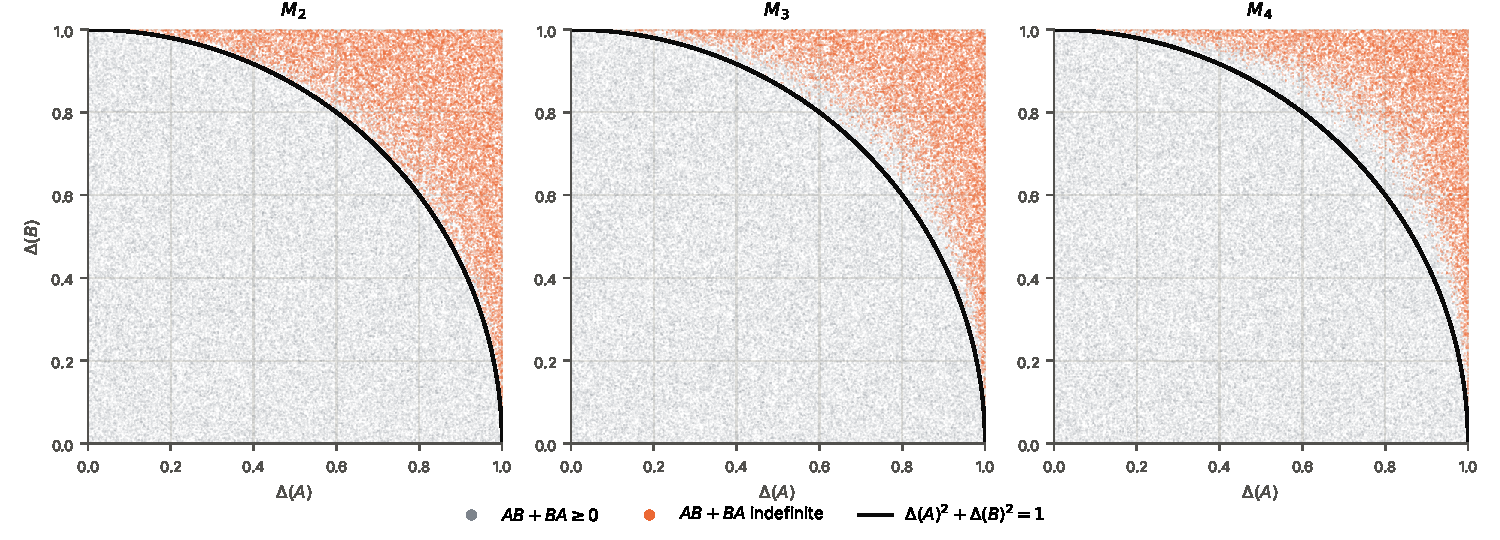
\includegraphics[width=\textwidth]{ops_jordan_positivity.pdf}
\caption[]{Is $AB+BA$ positive? $\COSamples$ random pairs $A,B>0$ per dimension, with contrasts uniform in $[0,1]^2$ and
Haar random relative position: positive (grey) or indefinite (orange). No indefinite product occurs inside the quarter
circle $\Delta(A)^2+\Delta(B)^2=1$ (Theorem~\ref{thm:jordan}(a)); outside it occurs for some positions, more often the
further out.}
\label{fig:ops-positivity}
\end{figure}

\begin{theorem}[Jordan product]\label{thm:jordan}
Let $A,B>0$ in $M_n$, $n\ge2$, with contrasts $\delta_A,\delta_B$, angles $\psi_A=\arcsin\delta_A$, $\psi_B=\arcsin\delta_B$
and rapidities $\eta_A=\operatorname{artanh}\delta_A$, $\eta_B=\operatorname{artanh}\delta_B$.
\begin{enumerate}
\item[(a)] $AB+BA\ge0$ for every relative position of $A$ and $B$ if and only if $\delta_A^2+\delta_B^2\le1$. If
$\delta_A^2+\delta_B^2>1$, $AB+BA$ is indefinite for some relative position, in every dimension.
\item[(b)] If $\delta_A^2+\delta_B^2<1$, then $\tanh|\eta_A-\eta_B|\le\Delta(AB+BA)\le\sin(\psi_A+\psi_B)$, and the lower
bound is attained by commuting $A,B$ whose extreme eigenvectors are interchanged.
\end{enumerate}
\end{theorem}
\begin{proof}
(a) and the upper bound in (b). We use the real angle $\angle(x,y)$ defined above. By the formula for $\cos\psi$,
$\angle(x,Bx)\le\psi_B$ and $\angle(Bx,ABx)\le\psi_A$, so $\angle(x,ABx)\le\psi_A+\psi_B$ by the triangle inequality;
likewise $\angle(x,BAx)\le\psi_A+\psi_B$. If $\psi_A+\psi_B<\frac\pi2$, the cone $\{y:\angle(x,y)\le\psi_A+\psi_B\}$ is
convex and contains $(AB+BA)x$, so $\langle(AB+BA)x,x\rangle>0$; moreover the largest angle of $AB+BA$ is at most
$\psi_A+\psi_B$, and its sine is $\Delta(AB+BA)$. The case $\psi_A+\psi_B=\frac\pi2$ follows by continuity.

Converse in (a). On $M_2$ take $A=\mathrm{diag}(1,a)$ and $B$ with eigenvalues $1,b$ and eigenvector
$(\cos\theta,\sin\theta)$ for $1$, where $a=\frac{1-\delta_A}{1+\delta_A}$, $b=\frac{1-\delta_B}{1+\delta_B}$. With
$c=\cos^2\theta$ and $p=(1-a)(1-b)$ a direct computation gives
\[
  \tfrac12\Tr(AB+BA)=a+b+pc,\qquad\det(AB+BA)=4ab-p^2c(1-c).
\]
At $\theta=\pi/4$ the determinant is negative if and only if $16ab<p^2$; with $\sqrt a=\sqrt{1-\delta_A^2}/(1+\delta_A)$ and
$1-a=2\delta_A/(1+\delta_A)$ this reads $(1-\delta_A^2)(1-\delta_B^2)<\delta_A^2\delta_B^2$, i.e.\ $\delta_A^2+\delta_B^2>1$.
On $M_n$ add the direct summands $a\,1_{n-2}$ and $b\,1_{n-2}$.

Lower bound in (b). If $x,y$ are unit eigenvectors of $A$ for its extreme eigenvalues $M_A$, $m_A$, then
$\lambda_{\max}(AB+BA)\ge2\Re\langle Bx,Ax\rangle=2M_A\langle Bx,x\rangle\ge2M_Am_B$ and likewise
$\lambda_{\min}(AB+BA)\le2m_AM_B$. So the condition number of $AB+BA$ is at least $h_A/h_B$, and by symmetry at least
$h_B/h_A$.
\end{proof}

How large can $\Delta(AB+BA)$ be? The upper bound $\sin(\psi_A+\psi_B)$ is reached only at the boundary of the disc. The
true maximum depends on the dimension, because in $M_2$ both extreme eigenvalues of $AB+BA$ come from the same pair of
$2\times2$ matrices, while in $M_3$ they can come from different blocks.

\begin{proposition}[Largest contrast of the Jordan product]\label{prop:jordanmax}
In the notation of the proof above, let $\delta_A^2+\delta_B^2<1$.
\begin{enumerate}
\item[(a)] On $M_2$, $\displaystyle\max\Delta(AB+BA)=\max_{0\le c\le1}\Bigl(1-\frac{4ab-p^2c(1-c)}{(a+b+pc)^2}\Bigr)^{1/2}$.
\item[(b)] On $M_n$, $n\ge3$, $\max\Delta(AB+BA)\ge(2-\mu)/(2+\mu)$, where
$\mu=\min_{0\le c\le1}\bigl(a+b+pc-\sqrt{(a+b+pc)^2-4ab+p^2c(1-c)}\,\bigr)$ is the smallest eigenvalue of $AB+BA$ over the
$2\times2$ pairs of (a).
\end{enumerate}
Numerically, both values equal the commuting value $\tanh(\eta_A+\eta_B)$ for small contrasts and exceed it for large ones.
\end{proposition}
\begin{proof}
(a) On $M_2$ every pair is unitarily equivalent to the pair of the proof of Theorem~\ref{thm:jordan} for some $\theta$,
and $\Delta^2=1-4\det/\Tr^2$. (b) Take $A=1\oplus A_2$ and $B=1\oplus B_2$ (padded with ones) with the $2\times2$ pair
$A_2,B_2$ of smallest eigenvalue $\mu$. Then $AB+BA=2\oplus(A_2B_2+B_2A_2)$ has the largest eigenvalue $2$, since
$\|A_2B_2+B_2A_2\|\le2$, and the smallest eigenvalue $\mu$.
\end{proof}

For $\delta_A=\delta_B=0.6$: the commuting value is $\COJordanTanh$, the maximum on $M_2$ is $\COJordanTwo$, the value of (b)
for $n\ge3$ is $\COJordanThree$, and $\sin(\psi_A+\psi_B)=\COJordanSin$. A numerical optimisation over all relative
positions and intermediate eigenvalues (\texttt{scripts/\allowbreak contrast\_\allowbreak operations.py}, 24 starts per point)
finds on $M_3$ and on $M_4$ exactly the value of (b) (largest difference $\COJordanDev$ on a grid of $\delta_A$ with
$\delta_B=0.6$; Figure~\ref{fig:ops-jordan}). Equality for every $n\ge3$ would follow if the smallest eigenvalue of a
Jordan product with spectra in $[a,1]$ and $[b,1]$ were always minimised on a two-dimensional subspace, the setting of
Strang's eigenvalue bounds~\cite{strang1962}; we do not use this.

The theorem explains a threshold. The analogue of item~21 for positive operators, $\varphi(\Re AB)\ge0$, holds for every
positive functional as long as $\Delta(A)^2+\Delta(B)^2\le1$, because then $\Re AB\ge0$; for operators of the same
contrast $\delta'$ it can fail only for $\delta'>1/\sqrt2$. For projections, $\psi=\frac\pi2$, and $\Re PQ$ is indefinite
in general; this is why item~21 is violated by every non-tracial functional, with the envelope $\frac12\tan^2(\psi/2)$
of Theorem~B.

\begin{proposition}[Commutators: three contrasts multiply]\label{prop:commutator}
Let $A,B>0$ in $M_n$.
\begin{enumerate}
\item[(a)] $\|AB-BA\|\le2\Delta(A)\Delta(B)\,m(A)m(B)$, with equality for suitable $A,B$ of any prescribed contrasts in
every $M_n$, $n\ge2$. In particular $\|AB-BA\|\le\frac{2\Delta(A)\Delta(B)}{(1+\Delta(A))(1+\Delta(B))}\|A\|\|B\|\le
\frac12\|A\|\|B\|$.
\item[(b)] For a state $\varphi_W$ ($\Tr W=1$) with $\Delta(W)=\delta$, $h=\frac{1+\delta}{1-\delta}$,
\[
  |\varphi_W(AB-BA)|\le2\,c_n(\delta)\,\Delta(A)\Delta(B)\,m(A)m(B),\qquad
  c_n(\delta)=\begin{cases}\delta,&n\ \text{even},\\[2pt] \dfrac{k(h-1)}{k(h+1)+1},&n=2k+1,\end{cases}
\]
and the bound is attained for every $\delta$ and all prescribed contrasts of $A$ and $B$.
\end{enumerate}
\end{proposition}
\begin{proof}
(a) Write $A=m(A)(1+E)$, $B=m(B)(1+F)$ with self-adjoint $E,F$, $\|E\|=\Delta(A)$, $\|F\|=\Delta(B)$. Then
$AB-BA=m(A)m(B)(EF-FE)$ and $\|EF-FE\|\le2\|E\|\|F\|$. Equality holds on $M_2$ for $E=\Delta(A)\sigma_z$,
$F=\Delta(B)\sigma_x$, since $\sigma_z\sigma_x-\sigma_x\sigma_z=2i\sigma_y$; in $M_n$ add a direct summand $m(A)\oplus m(B)$.
The second form uses $\|A\|=m(A)(1+\Delta(A))$. (b) $C=i(AB-BA)$ is self-adjoint with $\Tr C=0$ and $\|C\|\le K$, the bound
of (a). By von Neumann's trace inequality~\cite{bhatia1997}, $|\Tr WC|$ is at most the maximum of
$\sum_iw_ic_i$ over decreasingly ordered $w_i$ (the eigenvalues of $W$) and $c_i\in[-K,K]$ with $\sum_ic_i=0$, which is
$K\sum_{i\le k}(w_i-w_{n+1-i})$, $k=\lfloor n/2\rfloor$. Let $a=w_1$, $b=w_n=a/h$ and $S=\sum_{i\le k}w_i\le ka$. Then
$\sum_{i\le k}(w_i-w_{n+1-i})\le S-kb$ and $1=\Tr W\ge S+(n-k)b$. Maximising $S-kb$ under $S\le khb$ and $S\le1-(n-k)b$ gives
the value at $khb=1-(n-k)b$, namely $k(h-1)/(kh+n-k)$, which is $c_n(\delta)$ for even and odd $n$. For equality take $k$
copies of the $2\times2$ pair of (a), $W$ diagonal in the eigenbasis of the $k$ blocks of $C$ with the eigenvalues $a$ on the
positive and $b$ on the negative eigenvectors of $C$, and, for odd $n$, the eigenvalue $b$ of $W$ and scalars $A$, $B$ on
the remaining one-dimensional block.
\end{proof}

So the most basic characterisation of the trace, $\varphi(AB)=\varphi(BA)$, fails at the order of the product of three
contrasts, $2\Delta(W)\Delta(A)\Delta(B)$ in even dimension: the thesis~(I) in its simplest form. The odd dimensions are
slightly weaker, as for Gardner's inequality (Theorem~\ref{thm:gardnerD}), and $c_{2k+1}(\delta)\to\delta$ as $k\to\infty$.

Figures~\ref{fig:ops-sum}--\ref{fig:ops-commutator} compare random samples ($\COSamples$ per figure and dimension, Haar
random relative positions, the intermediate eigenvalues uniform between the extreme ones) with these bounds on $M_2$,
$M_3$ and $M_4$. No sample exceeds a bound (the largest value of sample minus bound is $\COWorst$). Among
$\COSamples$ further random pairs per dimension with contrasts uniform in $[0,1]^2$, the number of indefinite Jordan
products with $\delta_A^2+\delta_B^2\le1$ is $\COIndefInside$. As in Section~\ref{sec:montecarlo}, random positions rarely come close to the extremes in higher
dimension: for the commutator test on $M_4$ the samples stay far below the bound, which needs two aligned $2\times2$
blocks.

\begin{figure}[!htbp]
\centering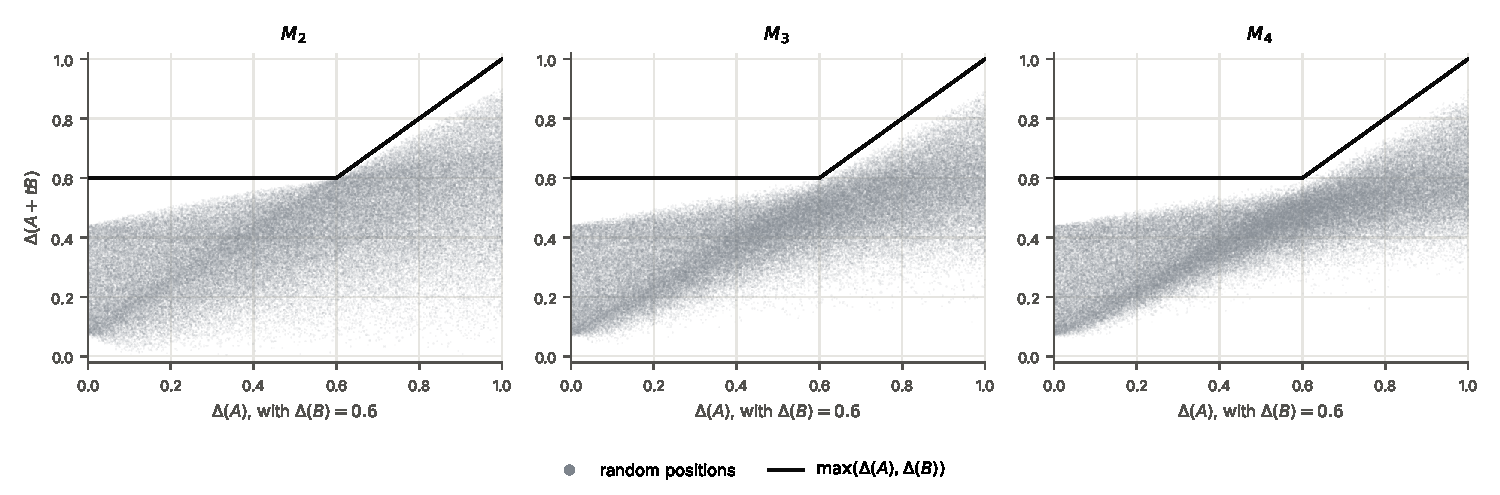
\includegraphics[width=\textwidth]{ops_sum.pdf}
\caption[]{Contrast of $A+tB$ ($t$ log-uniform) against $\Delta(A)$, with $\Delta(B)=0.6$: it never exceeds
$\max(\Delta(A),\Delta(B))$ (Proposition~\ref{prop:rapid}(d)).}
\label{fig:ops-sum}
\end{figure}
\begin{figure}[!htbp]
\centering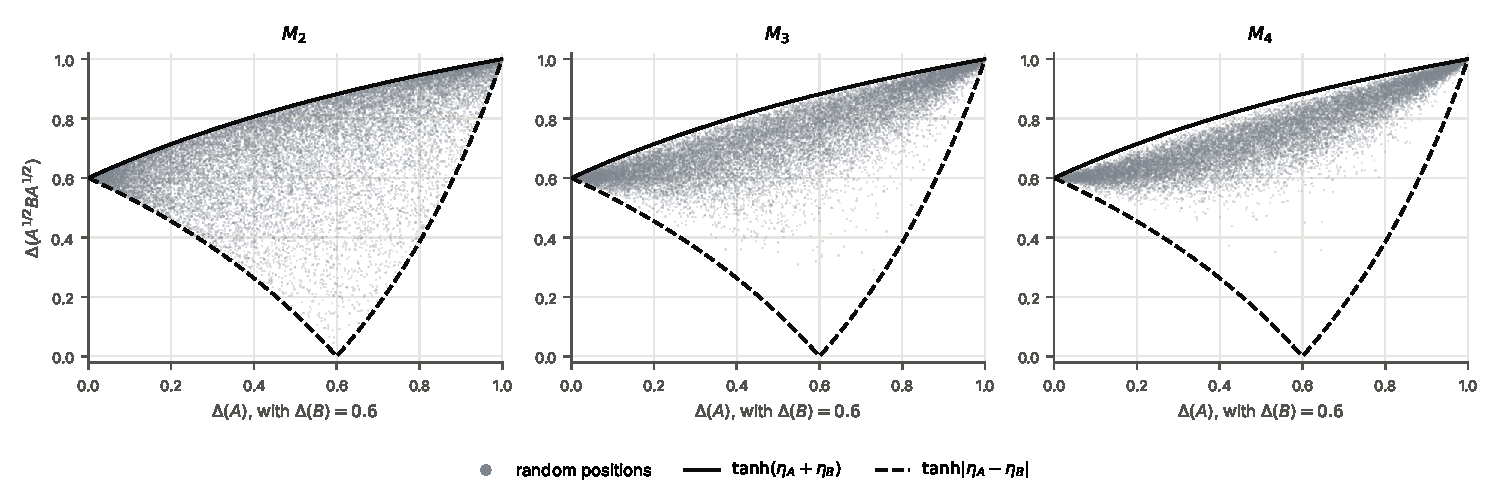
\includegraphics[width=\textwidth]{ops_congruence.pdf}
\caption[]{Contrast of $A^{1/2}BA^{1/2}$ against $\Delta(A)$, with $\Delta(B)=0.6$, and the bounds
$\tanh|\eta_A\pm\eta_B|$ of Proposition~\ref{prop:rapid}(b).}
\label{fig:ops-congruence}
\end{figure}
\begin{figure}[!htbp]
\centering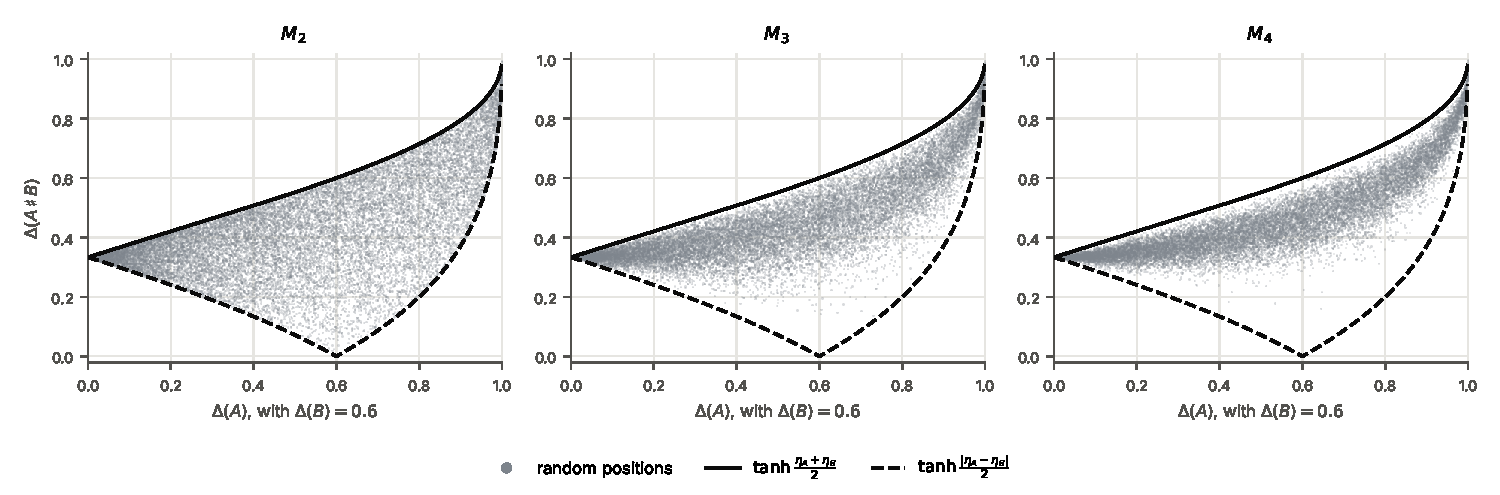
\includegraphics[width=\textwidth]{ops_geomean.pdf}
\caption[]{Contrast of the geometric mean $A\#B$ against $\Delta(A)$, with $\Delta(B)=0.6$, and the bounds
$\tanh\frac12|\eta_A\pm\eta_B|$ of Proposition~\ref{prop:rapid}(c).}
\label{fig:ops-geomean}
\end{figure}
\begin{figure}[!htbp]
\centering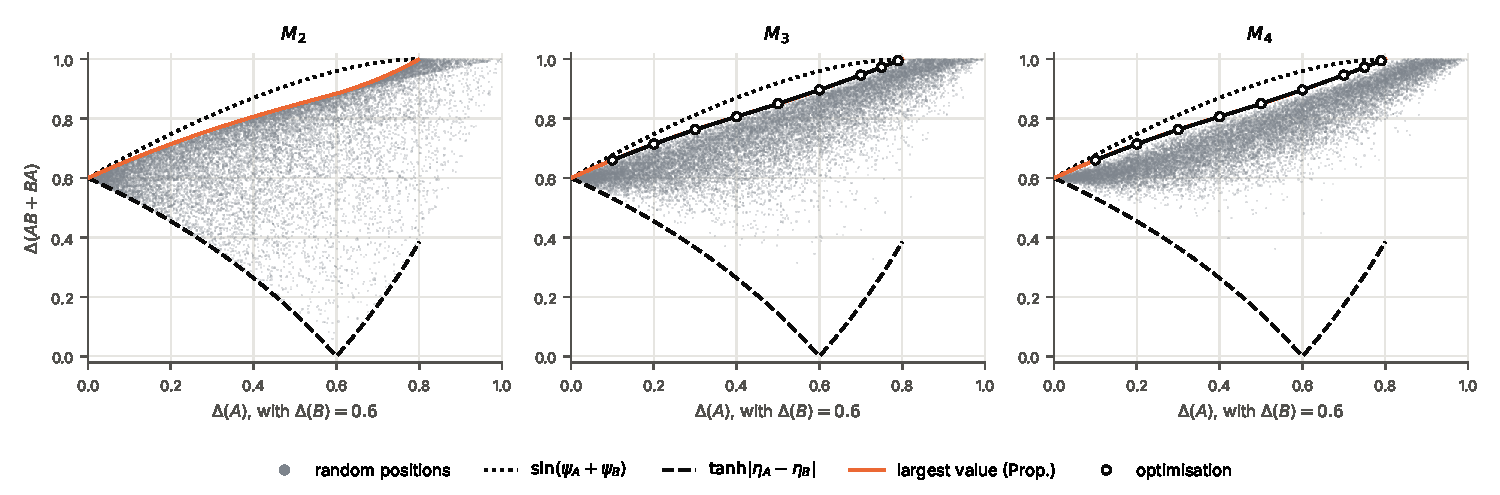
\includegraphics[width=\textwidth]{ops_jordan.pdf}
\caption[]{Contrast of the Jordan product $AB+BA$ against $\Delta(A)<0.8$, with $\Delta(B)=0.6$ (for $\Delta(A)\le0.8$ it
is positive, Theorem~\ref{thm:jordan}(a)): the bounds of Theorem~\ref{thm:jordan}(b), the largest value of
Proposition~\ref{prop:jordanmax} (orange; on $M_3$ and $M_4$ the value $(2-\mu)/(2+\mu)$), and the largest value found by
optimisation (markers).}
\label{fig:ops-jordan}
\end{figure}
\begin{figure}[!htbp]
\centering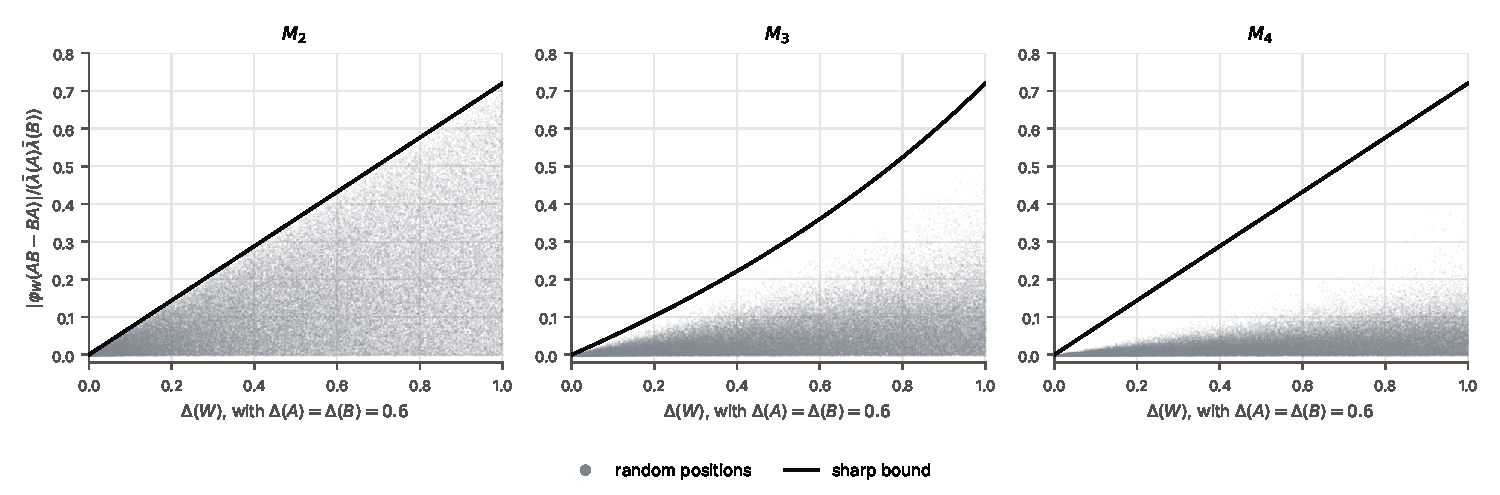
\includegraphics[width=\textwidth]{ops_commutator.pdf}
\caption[]{The commutator test $|\varphi_W(AB-BA)|/(m(A)m(B))$ for states $\varphi_W$ against $\Delta(W)$, with
$\Delta(A)=\Delta(B)=0.6$, and the sharp bound $2c_n(\delta)\cdot0.36$ of Proposition~\ref{prop:commutator}(b).}
\label{fig:ops-commutator}
\end{figure}

\section{Numerical verification and the remaining items}\label{sec:numerics}

\subsection{Method}
All envelopes were computed by constrained optimisation with our PyTorch library \texttt{torch\_\allowbreak vn\_\allowbreak algebra}~\cite{lib}; the program is \texttt{scripts/\allowbreak trace\_\allowbreak characterizations.py} of the
repository~\cite{lib}. The density $W$ is diagonal with a spectrum parametrised so that $\Delta(W)=\delta$ holds exactly
and the other eigenvalues are free. Positive variables have a free contrast in $[0,1]$, so rank-deficient operators are
included; there are self-adjoint and unitary variables (polar factors, and projections $UDU^*$, with every rank pattern
spread over the starts), and positive scalars. Half of the starts begin at structured points (two-level spectra, rotations
in pairs of eigenvectors of $W$). The lattice operations are the spectral projections of $P+Q$ for the eigenvalue $2$ ($P\wedge
Q$) and for the range ($P\vee Q$), computed by functional calculus with an indicator function, whose Daleckii--Krein
gradient is the derivative of the spectral projection. In 19 and~23 the suprema are approached as $P$ and $Q$ merge, where
$P\wedge Q$ and $P\vee Q$ jump; there the search maximises $(L-R)/N-10^{-12}/\|P-Q\|_{\mathrm F}^2$, which keeps $P$ and $Q$
about $10^{-3}$ apart, while the reported values are those of $(L-R)/N$. A grid of $\TCGridSize$ contrasts times
$\TCStarts$ starts forms one batch per item and dimension ($\TCSteps$ gradient steps, $n=\TCDims$).

\emph{Certification.} The best final point of every contrast is recomputed in mpmath with $\TCDigits$ digits, after the
unitaries are re-orthonormalised and the contrast is recomputed from the stored eigenvalues; the lattice operations are
recomputed from the exact eigenvalues. Every positive value reported below is thus a certified violation at an exactly
admissible point. The double-precision and mpmath values agree to $\TCCertDev$ (relative), and at $\delta=0$ no value
exceeds $\TCVzero$. Independently, plain NumPy/SciPy searches (BFGS from $\TCSciStarts$ random starts on $M_2$ at
$\delta=0.3,0.5,0.9$) give values whose ratio to the batched search lies in $[\TCSciRatioMin,\TCSciRatioMax]$; ratios above
$1$ come from item~13, where BFGS stops earlier. The test suite compares every objective with a plain NumPy implementation
and with mpmath, checks that random points stay below the proved envelopes and that the stated extremisers attain them.
The whole computation takes $\TCSeconds$~s on $\TCWorkers$ CPU processes.

\subsection{Random sampling}\label{sec:montecarlo}

Before searching for the extremes we sample. A third program (\texttt{scripts/\allowbreak trace\_\allowbreak
montecarlo.py}, plain NumPy, independent of the library) draws, for each of the 25 items and for $n=\TMCDims$,
$\TMCSamples$ random functionals on $M_n$ and random operators: $W$ with a uniformly distributed contrast
$\Delta(W)\in[0,1)$ and the other eigenvalues uniform in between, positive operators $U\mathrm{diag}(\lambda)U^*$ with
Haar-random $U$, a uniformly distributed contrast and a random scale, arbitrary operators $V|X|$ with a Haar-random $V$,
self-adjoint ones with random signs, and Haar-random projections. This is the method of~\cite[Sect.~5]{abed2024},
extended to all items. A second sample replaces every positive operator (every modulus) by a scaled projection of
random rank (\emph{projection sample}). Appendix~\ref{app:mc} has one figure per item with one panel per dimension:
every sample, $(L-R)/N$ against $\Delta(W)$, together with the certified envelope $V(\delta)$. For the 14 items with
operator variables a second row shows a third sample, with $\Delta(W)=0.9$ and all operator variables of one contrast
$\delta'$, against $\delta'$, together with the certified $V(0.9,\delta')$ of Section~\ref{sec:bothcontrasts}.
Table~\ref{tab:montecarlo} gives the fraction of violating samples.

\begin{table}[h]
\centering\small
\setlength{\tabcolsep}{4pt}
\begin{tabular}{rl|rr|rr|rr}
\toprule
 & & \multicolumn{2}{c|}{$M_2$} & \multicolumn{2}{c|}{$M_3$} & \multicolumn{2}{c}{$M_4$}\\
item & inequality & random & proj. & random & proj. & random & proj.\\
\midrule
\TMCRows
\bottomrule
\end{tabular}
\caption[]{Random sampling, $\TMCSamples$ samples per item, class and dimension: the percentage of samples that violate
the inequality, for random operators and for scaled projections. ``--'': not applicable (the variables are projections,
or an invertible operator is needed).}
\label{tab:montecarlo}
\end{table}

The samples show four things.
\begin{enumerate}
\item[(a)] \emph{No sample exceeds the envelope}: the largest ratio of a sampled violation to the certified envelope at
the upper edge of its bin is $\TMCWorstRel$ over all items and dimensions (the excess over $1$ is the linear
interpolation between grid values of the envelope). This is an independent check of the computed envelopes.
\item[(b)] \emph{Random operators rarely come close to the envelope}, and for monotonicity, subadditivity, the
Powers--St{\o}rmer inequality and the weighted monotonicity essentially never violate it: less than $0.1\%$ of the
samples (or none) violate. A Monte Carlo study alone would conclude that these inequalities hold for every $\varphi_W$.
\item[(c)] \emph{Sampling gets worse with the dimension}: for Gardner's inequality the fraction of violating random samples
drops from $4.4\%$ on $M_2$ to below $0.1\%$ on $M_3$ and on $M_4$, and the best sample stays
far below the envelope (Figure~\ref{fig:mc-gardner}). The extremal configurations, rank-one operators on a two-dimensional
subspace aligned with the extreme eigenvectors of $W$, have a Haar measure that decreases rapidly with $n$.
\item[(d)] \emph{Projections detect the failure.} Sampling scaled projections instead of general positive operators raises
the fraction of violating samples in every dimension, for Gardner's inequality from $4.4\%$ to $19\%$ on $M_2$ and from
below $0.1\%$ to $0.6\%$ on $M_4$, for subadditivity from below $0.1\%$ to $21\%$, $9\%$ and $5\%$ on $M_2$, $M_3$, $M_4$, for the
power-mean inequality from $7\%$ to $50\%$ on $M_2$, and brings the best sample close to the envelope (orange points in Figures~\ref{fig:mc-gardner},
\ref{fig:mc-subadd} and~\ref{fig:mc-lp}). The exceptions are those of Section~\ref{sec:projsuffice}: for items 4 and~7 the extremisers are
two-level operators that are not projections (for item~7 the violation degenerates exactly at projections), and items 6
and~11 need invertible operators.
\end{enumerate}

\subsection{Do projections suffice?}\label{sec:projsuffice}

For the 14 items whose variables are not projections, a second program (\texttt{scripts/\allowbreak trace\_\allowbreak contrast.py}) repeats the
search with the positive variables (the moduli, for the others) restricted in two ways: to two-level operators
$c(\ell+(1-\ell)P)$ with free $\ell\in[0,1]$, $c>0$ and a projection $P$ of any rank (for self-adjoint variables $\alpha+\beta P$
with free real $\alpha,\beta$), and to scaled projections $cP$. Everything else is as before ($\TCCStarts$ starts per grid
point, $\TCCSteps$ gradient steps, best final point recomputed in mpmath with $\TCCDigits$ digits); the whole computation of
this and the next subsection takes $\TCCSeconds$~s on four CPU processes.

\begin{table}[h]
\centering\scriptsize
\setlength{\tabcolsep}{3pt}
\begin{tabular}{r|ccc|ccc|ccc|ccc}
\toprule
 & \multicolumn{6}{c|}{$M_2$} & \multicolumn{6}{c}{$M_3$}\\
 & \multicolumn{3}{c|}{$\delta=0.5$} & \multicolumn{3}{c|}{$\delta=0.9$} & \multicolumn{3}{c|}{$\delta=0.5$} &
 \multicolumn{3}{c}{$\delta=0.9$}\\
item & all & two-level & proj. & all & two-level & proj. & all & two-level & proj. & all & two-level & proj.\\
\midrule
\TCCRowsA
\bottomrule
\end{tabular}
\caption[]{Certified largest violations over all operators, over two-level operators and over scaled projections, for the
items whose variables are not projections. In $M_2$ every operator is two-level, so there the middle column only checks
the restricted parametrisation. ``--'': item~11 needs an invertible $A$.}
\label{tab:projsuffice}
\end{table}

Table~\ref{tab:projsuffice} shows four groups.
\begin{enumerate}
\item[(a)] \emph{Projections attain the envelope}: items 1, 2, 3, 8, 10, 12, 16 and~24 in $M_2$ and $M_3$ (item~16 to
within $0.3\%$), and item~13 in $M_2$. Together with the 11 items whose variables are projections by definition, this covers 20 of the 25 items.
\item[(b)] \emph{Projections approach it}: in items 6 and~7 the supremum is approached as an operator becomes a
projection, where both sides of the inequality degenerate. Restricted to projections (item~6) or to two-level operators
(item~7), the search comes closer to the proved lower bound $\kappa-1$, resp.\ $\kappa^2-1$, than without restriction:
the restriction helps the search.
\item[(c)] \emph{Two-level operators are needed}: item~4 (the extremiser $A=\sqrt a\,e_1e_2^*+\sqrt b\,e_2e_1^*$ has
$|A|$ with the eigenvalues $\sqrt a,\sqrt b$), item~11 ($A=W^{-1}$) and item~25 ($A$ with the eigenvalue ratio $\approx\delta^2/8$,
Proposition~\ref{prop:wmon}; rank-one $A$ gives no violation). In $M_3$ the extremiser of item~4 lives on a
two-dimensional subspace and vanishes on its complement, so it has three eigenvalues $\sqrt a,\sqrt b,0$; the two-level
class without $0$ misses it.
\item[(d)] \emph{Exceptions}: in $M_3$ at $\delta=0.9$ the generalised Powers--St{\o}rmer inequality (item~13) is violated by
$0.3048$ against $0.2197$ for projections and for $M_2$, and the spectral geometric mean (item~6) exceeds $\kappa-1$ for
$n\ge3$ (Section~\ref{sec:numerics}, item (iii) below). Here operators that are not two-level do more.
\end{enumerate}

\subsection{Both contrasts}\label{sec:bothcontrasts}

The bottom rows of Figures~\ref{fig:mc-gardner}--\ref{fig:mc-wmon} (Appendix~\ref{app:mc}) show $V(0.9,\delta')$ for the same 14 items, with random samples. At $\delta'=0$ no item is violated
(Proposition~\ref{prop:scalar}). Beyond that, the items fall into four classes.
\begin{enumerate}
\item[(a)] \emph{Smooth growth in both contrasts}: items 1--3 follow Theorem~\ref{thm:gardnerD} to $\TCCGardnerDev$
(relative, $n=2,3$, all grid points); item~8 follows Proposition~\ref{prop:youngtwo} on $M_2$.
\item[(b)] \emph{A threshold in the contrast of the operators}: items 6, 10, 12, 13, 24 and~25 show no violation until
$\delta'$ is close to $1$; at $\delta=0.9$ the first grid value with a violation above $10^{-4}$ is: \TCCThresholds. These
characterisations are blind to operators of moderate contrast: their violation needs nearly singular operators.
\item[(c)] \emph{A peak}: item~11 is violated most strongly when the contrast of $A$ is close to that of $W$ (its
extremiser is $W^{-1}$), and in $M_2$ items 4 and~7 have an interior maximum in $\delta'$ (for item~4 at the contrast of
$|A|$ of the extremiser in (c) above); in $M_3$ the additional dimension removes the maxima of 4 and~7.
\item[(d)] \emph{No dependence on the contrast of the operators}: item~16 is invariant under $A\mapsto A+c$,
$B\mapsto B+c$, which makes the contrasts of $A$ and $B$ arbitrarily small without changing the quotient; accordingly
$V(\delta,\delta')$ equals the envelope with free operators for every $\delta'>0$ and jumps to $0$ at $\delta'=0$.
\end{enumerate}
On $M_2$ every spectrum is two-level. On $M_3$ the two-level operators of contrast $\delta'$ reproduce the values of
general spectra with the same contrast except in items 4, 6 and~7 near $\delta'=1$: there the extremisers need a third
eigenvalue (a zero on the complement of a two-dimensional subspace, or a nearly singular second operator).

\subsection{Envelopes with the operators free}

\begin{table}[h]
\centering\scriptsize
\setlength{\tabcolsep}{4pt}
\begin{tabular}{llllll}
\toprule
items & $V^\star(\delta)$ & as $\delta\to0$ & $V^\star(0.5)$ & search $V(0.5)$ & status\\
\midrule
\TCClassRows
\bottomrule
\end{tabular}
\caption[]{Classes of behaviour, ordered by the order of vanishing of the envelope at the trace. $V^\star$: the sharp
value or, where marked $\ge$, a proved lower bound; ``search'': the certified search value on $M_2$ (a range over the
items of a row). Items 11 and 24 are given for $n=2$.}
\label{tab:classes}
\end{table}

\begin{table}[h]
\centering\scriptsize
\setlength{\tabcolsep}{1.8pt}
\begin{tabular}{rlccccccrc}
\toprule
 & inequality $L\le R$ & ref. & $V(0.1)$ & $V(0.5)$ & $V(0.9)$ & $V^\star(0.5)$ & order & slope & $n$-dep.\\
\midrule
\TCRows
\bottomrule
\end{tabular}
\caption[]{Certified search values on $M_2$ at $\delta=0.1,0.5,0.9$ and the proved values $V^\star$; $^a$: sharp for $n=2$
only, $^b$: a lower bound, $^c$: approached but not attained. ``order'': leading order of $V^\star$ as $\delta\to0$;
``slope'': $\log_2(V(0.2)/V(0.1))$ of the search; ``$n$-dep.'': the largest $|V_n/V_2-1|$ for $n=3,4$ and $\delta\ge0.1$ (for
item~7 it reflects search shortfalls, for item~13 a genuine increase with $n$; items 19 and 20 differ for odd $n$, Theorem~\ref{thm:proj}). ``n.r.'': no
violation resolved by the search ($\TCMode$ run on $\TCDevice$).}
\label{tab:values}
\end{table}

Tables~\ref{tab:classes} and~\ref{tab:values} and the top rows of Figures~\ref{fig:mc-gardner}--\ref{fig:mc-wmon} summarise the computation.

\begin{enumerate}
\item[(i)] \emph{Agreement with the theorems.} Where the envelope is known exactly and attained (items 1--5, 8, 11, and 9
for $n=2$), the search reproduces it to $\TCSharpDev$ for $\delta\ge0.05$ and $n=2,3,4$; for items 17, 18, 20--22 and 24
to $\TCSharpDevNew$, and for the approached suprema of 19 and 23 to $\TCSharpDevApproached$. Apart from item~6 with
$n\ge3$, no value exceeds the lower bounds of Section~\ref{sec:lower} (largest relative excess $\TCBoundExcess$). The
values of 17, 18 and 21--23 on $M_3$ and $M_4$ agree with the $M_2$ values to $\TCNDevNew$, as Theorem~\ref{thm:proj}
predicts, and the search on $M_3$ finds the odd-$n$ value $\TCExpOddHalf$ of item~20 at $\delta=0.5$ ($M_2$:
$\TCRefExpqpqHalf$).
\item[(ii)] \emph{Items without a closed form.} All five items 12--16 fail quadratically, with $V\approx0.5\,\delta^2$
(12, 13), $\delta^2/36$ (14, equal to the bound of Proposition~\ref{prop:lower}(d) to leading order), $0.064\,\delta^2$ (15)
and $0.09\,\delta^2$ (16). Item~15 decreases with $n$, because the identity part of $e^{P/2}e^Qe^{P/2}$ enters $N$;
item~13 increases with $n$ at large $\delta$ (on $M_3$ at $\delta=0.9$: $0.3048$ against $0.2197$ on $M_2$, both certified);
items 12, 14 and~16 give the same values for $n=2,3,4$. In item~16 the best points have large $\|A\|$, $\|B\|$, and the supremum is
approached as the scale grows.
\item[(iii)] \emph{Dimension.} For items 9 and 10 the search gives the same values for $n=3,4$ as for $n=2$, to $\TCNDev$.
Item~6 depends on $n$: for $n=2$ the search never exceeds $\kappa-1$, but for $n\ge3$ it certifies larger violations,
$V\ge\TCSGMExcessV$ at $n=\TCSGMExcessN$, $\delta=\TCSGMExcessDelta$, where $\kappa-1=\TCSGMExcessKappa$; a stored point gives
$V>2.1$ at $n=3$, $\delta=0.9$, where $\kappa-1=1.29$. We only know $\kappa-1\le V_6\le h-1$.
\item[(iv)] \emph{Extremisers.} Except for items 6 ($n\ge3$), 11 ($A=W^{-1}$) and 25 ($A$ of rank two with eigenvalue
ratio $\approx\delta^2/8$), the extremisers are rank-one operators or matrix units in the span of eigenvectors for $a$ and
$b$, and they do not commute with $W$.
\item[(v)] \emph{Limits of the search.} The suprema of 6 and 7 are approached only as an operator becomes singular;
gradient ascent reaches $\TCSGMRatioHalf$ and $\TCALTRatioHalf$ of the bound at $\delta=0.5$, and finds no violation of
item~6 for $\delta\le0.2$. Item~25 is resolved for $\delta\ge\TCWmonFirst$; the search reaches $m_{25}$ to $10^{-3}$ for
$\delta\ge\TCWmonReach$ and does not exceed it.
\item[(vi)] \emph{Direct sums.} On $M_2\oplus M_3$ with $W=1\oplus s1$ and $W=\mathrm{diag}(1,\ell)\oplus s1$, $s\in\{\frac14,4\}$,
intra-block contrast $\delta\in\{0.3,0.5,0.7\}$: for central $W$ the largest value found for the items that hold for every
trace is $\TCSectorCentral$; for 11 and 24 the search reproduces the exact values for the fixed density to $\TCSectorDet$;
with intra-block contrast no value exceeds the $M_2$ envelope (largest relative excess $\TCSectorExcess$), and where
Theorem~\ref{thm:sectors} gives equality the search reaches it to $10^{-3}$ in $\TCSectorReached$ of $\TCSectorTotal$ cases.
\end{enumerate}

\section{Conclusions and open problems}\label{sec:open}

For the 25 characterisations of the trace studied here, the violation of the inequality by a non-tracial functional
$\varphi_W$ is controlled by two Michelson contrasts, that of $W$ and that of the operators: it vanishes if either is
zero, and for Gardner's inequality and its relatives it is an explicit function of their product. The largest violation
is found, with few exceptions, at projections or at two-level operators $\ell+(1-\ell)P$, as the vertex principle predicts
where it applies. Testing a characterisation on projections and their affine images is therefore the efficient way to
detect a non-tracial functional, and the size of the violation measures the contrast of its density. The exceptions are
structural: thresholds in the contrast of the operators, a peak at the contrast of the density for the determinant
inequality, shift invariance for the Peierls--Bogoliubov inequality, and, in dimension three, the spectral geometric
mean and the generalised Powers--St{\o}rmer inequality. The contrast of composite operators follows simple rules
(Section~\ref{sec:composite}): rapidities add for products and means, angles add for Jordan products, and the commutator
test of traciality fails by the product of the three contrasts of $W$, $A$ and~$B$.


\begin{conjecture}
$V_n=\kappa^2-1$ for item~7, $V_n=m(\delta)$ for item~10 and $V_n=m_{25}(\delta)$ for item~25 in every dimension;
$V_2=\kappa-1$ for item~6; and the value of Proposition~\ref{prop:abed} holds for item~9 in every dimension.
\end{conjecture}

\noindent Further questions: (0) proofs of the threshold phenomenon of Section~\ref{sec:bothcontrasts}(b), i.e.\ of
inequalities that hold for every $\varphi_W$ as long as the operators have contrast below a critical value depending on
$\Delta(W)$, and of the equality in Proposition~\ref{prop:youngtwo}; (1) the envelope of item~6 for $n\ge3$, where the search exceeds $\kappa-1$, and whether it
grows with $n$; (2) closed forms for items 12--16, whose leading coefficients the search gives as $\frac12$, $\frac12$,
$\frac1{36}$, $0.064$ and $0.09$ (item 14: the leading coefficient $(1-\frac2p)^2/4$ is a lower bound); (3) the analogues
for infinite-dimensional von Neumann algebras, where the contrast of an unbounded density may be $1$ while the functional
is still close to a trace in other senses; (4) envelopes for other inequalities that characterise traces, e.g.\ those
of~\cite{moslehian2025jmaa,bikchentaev2026sgm} with the arithmetic mean, and for the dual problem of characterising
central elements~\cite{novikov2015}.

\paragraph{Code availability.} The library, the programs that compute all numbers, tables and figures, and the tests
are available at \url{https://github.com/andre-a-no/von_neumann_type_i} (MIT licence).

\clearpage
\appendix
\section{Random samples and certified envelopes, item by item}\label{app:mc}

Each figure belongs to one inequality and has one panel per dimension. Top row: the normalised violation $(L-R)/N$ of the
$\TMCSamples$ random samples (grey) and, where the variables are not projections, of the $\TMCSamples$ scaled-projection
samples (orange) against $\Delta(W)$ on $M_2$, $M_3$, $M_4$ (Section~\ref{sec:montecarlo}); black: the certified envelope
$V(\delta)$ on the grid of Section~\ref{sec:numerics}, joined by straight lines. Bottom row (items with operator
variables): random samples with $\Delta(W)=0.9$ and every operator variable of one contrast $\delta'$, against $\delta'$
on $M_2$ and $M_3$; black: the certified $V(0.9,\delta')$ of Section~\ref{sec:bothcontrasts}. Samples far below zero are
cut off. Where a curve is concave between grid points (item~11 below its maximum at $\delta'=\delta$, and after its
steep drop near $\delta'=1$) a few samples lie above the straight segments; on $M_2$ they lie below the closed form
$1-(w_1\ell'+w_2)/(2\sqrt{\ell'})$, $\ell'=\frac{1-\delta'}{1+\delta'}$, $w=\frac{2}{1+\ell}(1,\ell)$.

% generated by scripts/trace_montecarlo.py -- do not edit by hand
\begin{figure}[!htbp]
\centering
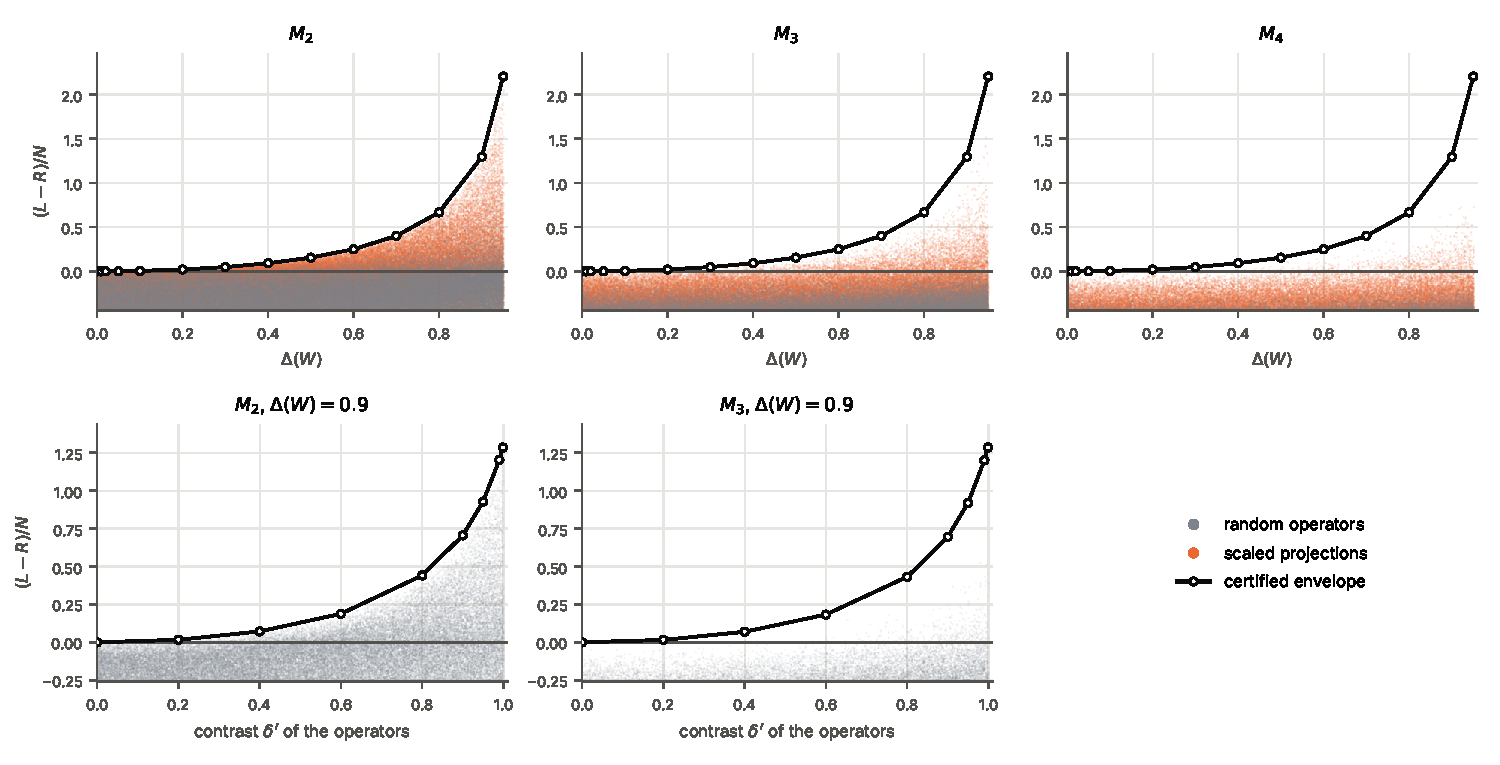
\includegraphics[width=\textwidth]{mc_01_gardner.pdf}
\caption[]{Item 1, $|\varphi(X)|\le\varphi(|X|)$: random samples and the computed envelope (a certified lower bound); top: against $\Delta(W)$, bottom: against the contrast $\delta^\prime$ of the operators at $\Delta(W)=0.9$.}
\label{fig:mc-gardner}
\end{figure}

\begin{figure}[!htbp]
\centering
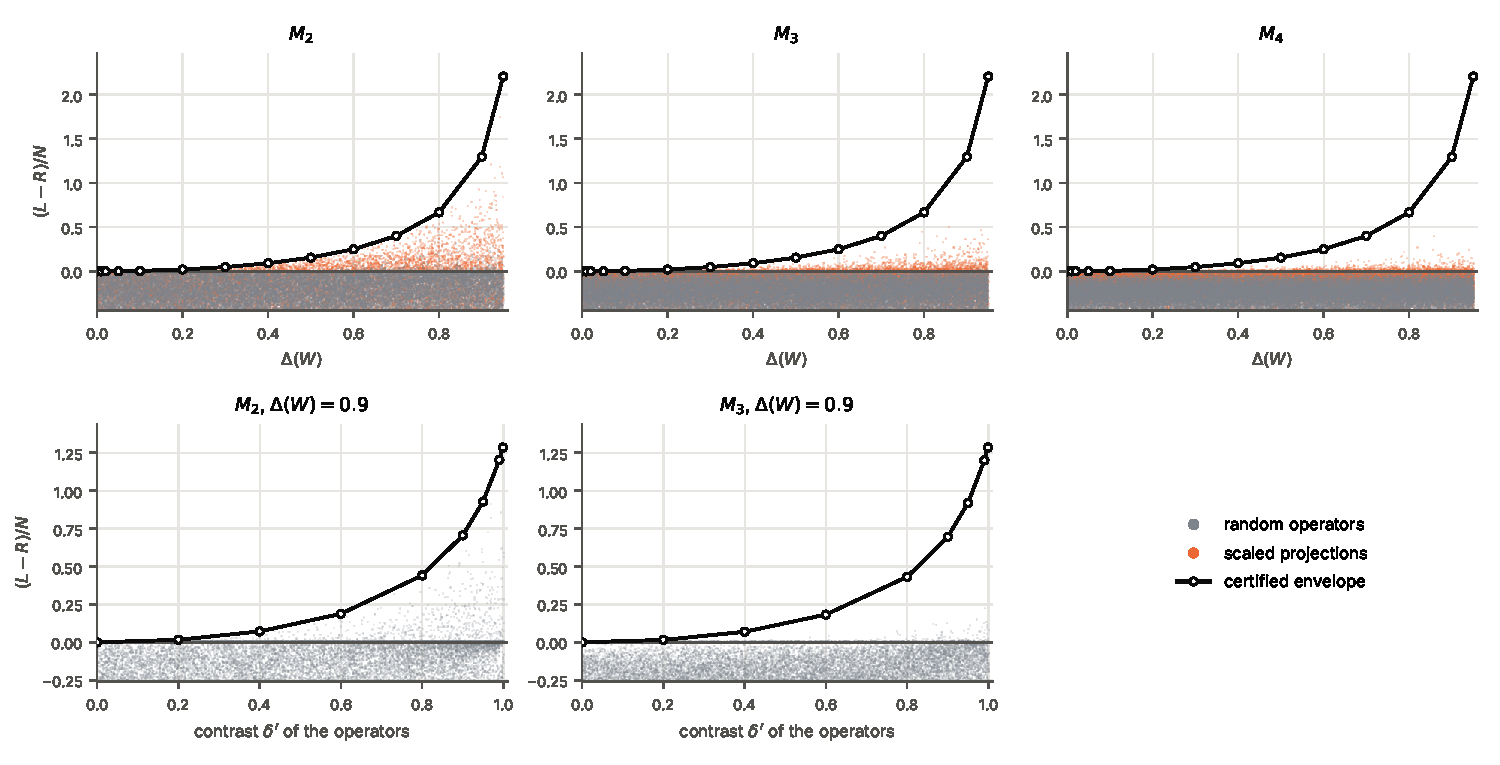
\includegraphics[width=\textwidth]{mc_02_triangle.pdf}
\caption[]{Item 2, $\varphi(|X+Y|)\le\varphi(|X|)+\varphi(|Y|)$: random samples and the computed envelope (a certified lower bound); top: against $\Delta(W)$, bottom: against the contrast $\delta^\prime$ of the operators at $\Delta(W)=0.9$.}
\label{fig:mc-triangle}
\end{figure}

\begin{figure}[!htbp]
\centering
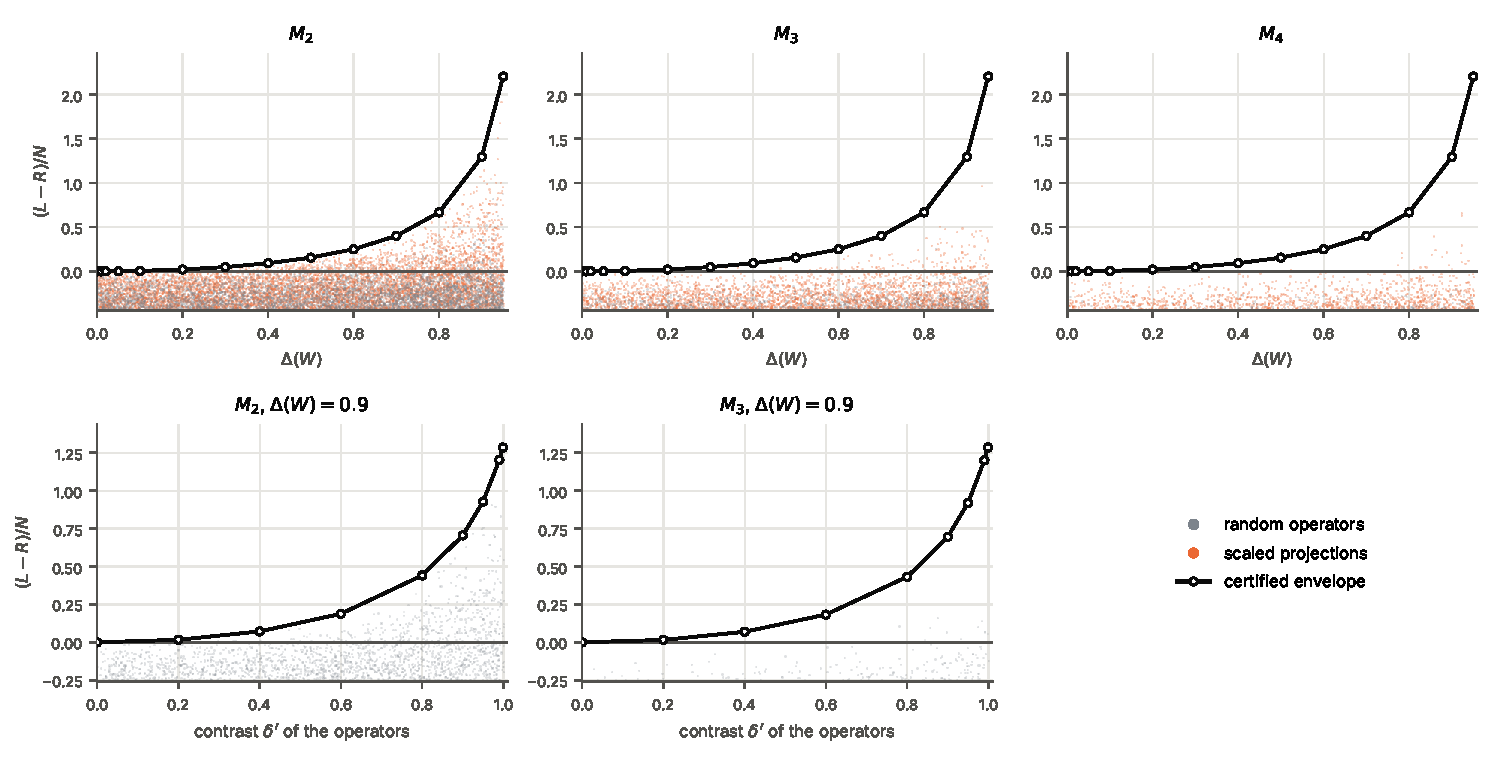
\includegraphics[width=\textwidth]{mc_03_realpart.pdf}
\caption[]{Item 3, $\varphi(A+A^*)\le2\varphi(|A^*|)$: random samples and the computed envelope (a certified lower bound); top: against $\Delta(W)$, bottom: against the contrast $\delta^\prime$ of the operators at $\Delta(W)=0.9$.}
\label{fig:mc-realpart}
\end{figure}

\begin{figure}[!htbp]
\centering
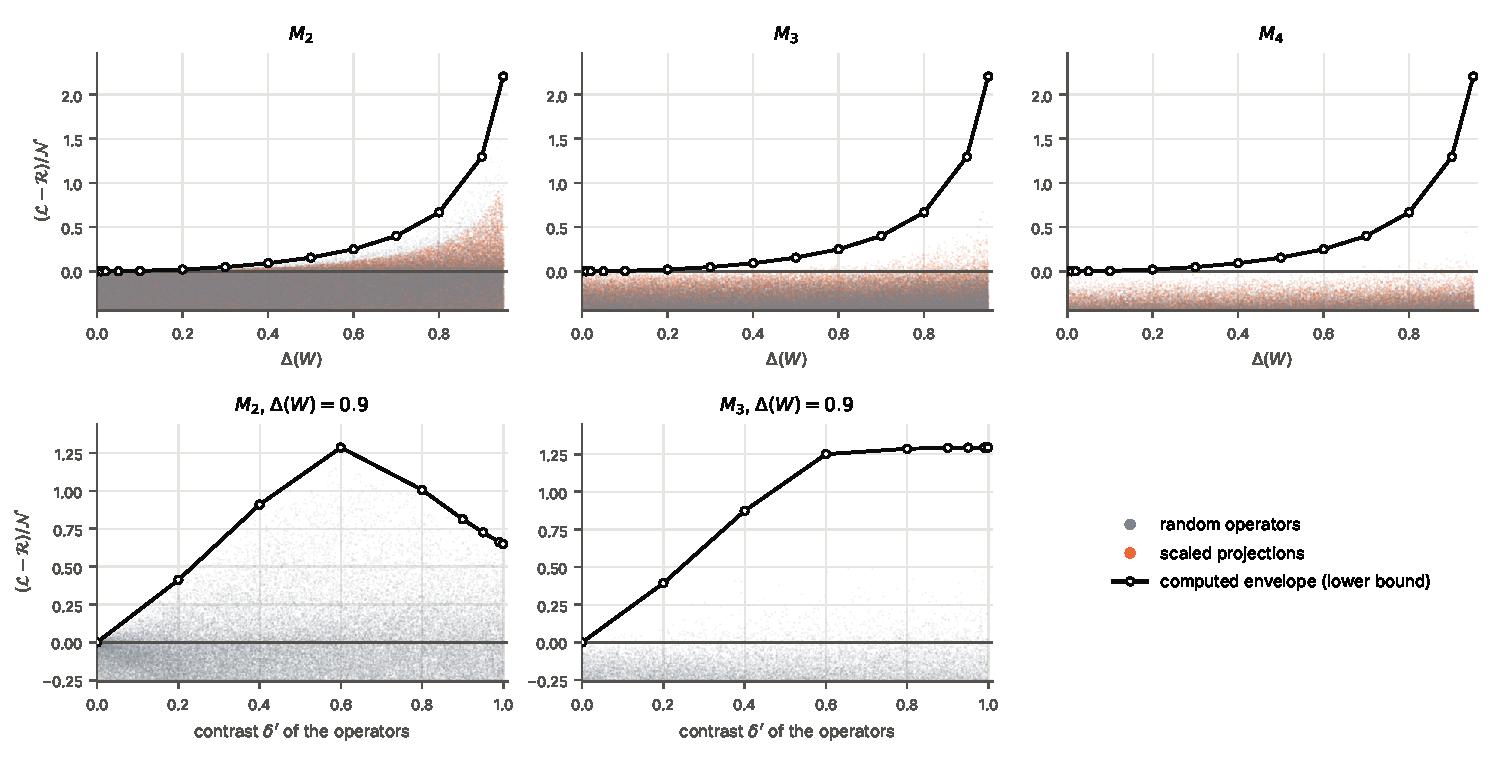
\includegraphics[width=\textwidth]{mc_04_square.pdf}
\caption[]{Item 4, $|\varphi(A^2)|\le\varphi(A^*A)$: random samples and the computed envelope (a certified lower bound); top: against $\Delta(W)$, bottom: against the contrast $\delta^\prime$ of the operators at $\Delta(W)=0.9$.}
\label{fig:mc-square}
\end{figure}

\begin{figure}[!htbp]
\centering
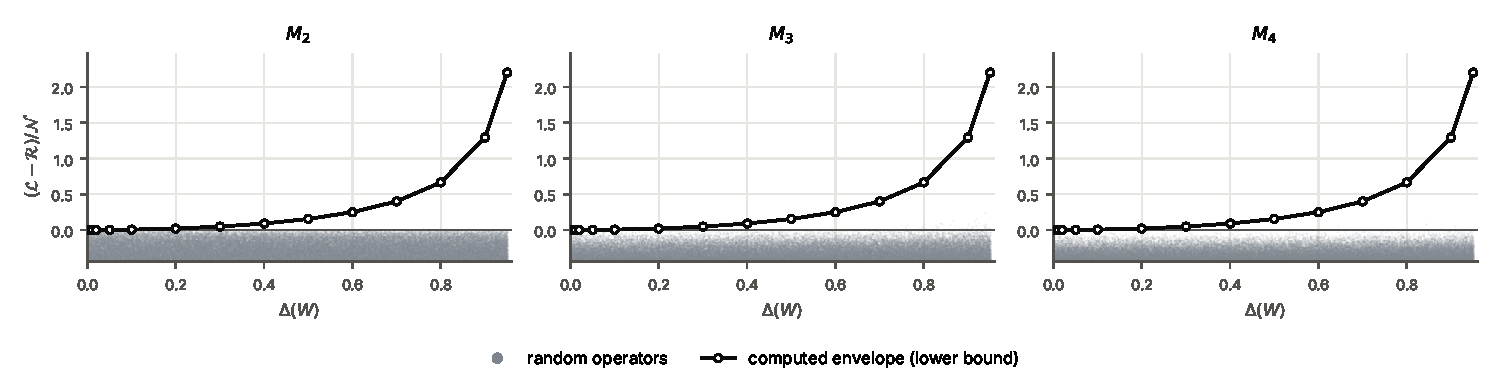
\includegraphics[width=\textwidth]{mc_05_metric.pdf}
\caption[]{Item 5, $\varphi(|P-R|)\le\varphi(|P-Q|)+\varphi(|Q-R|)$: random samples and the computed envelope (a certified lower bound) against $\Delta(W)$.}
\label{fig:mc-metric}
\end{figure}

\begin{figure}[!htbp]
\centering
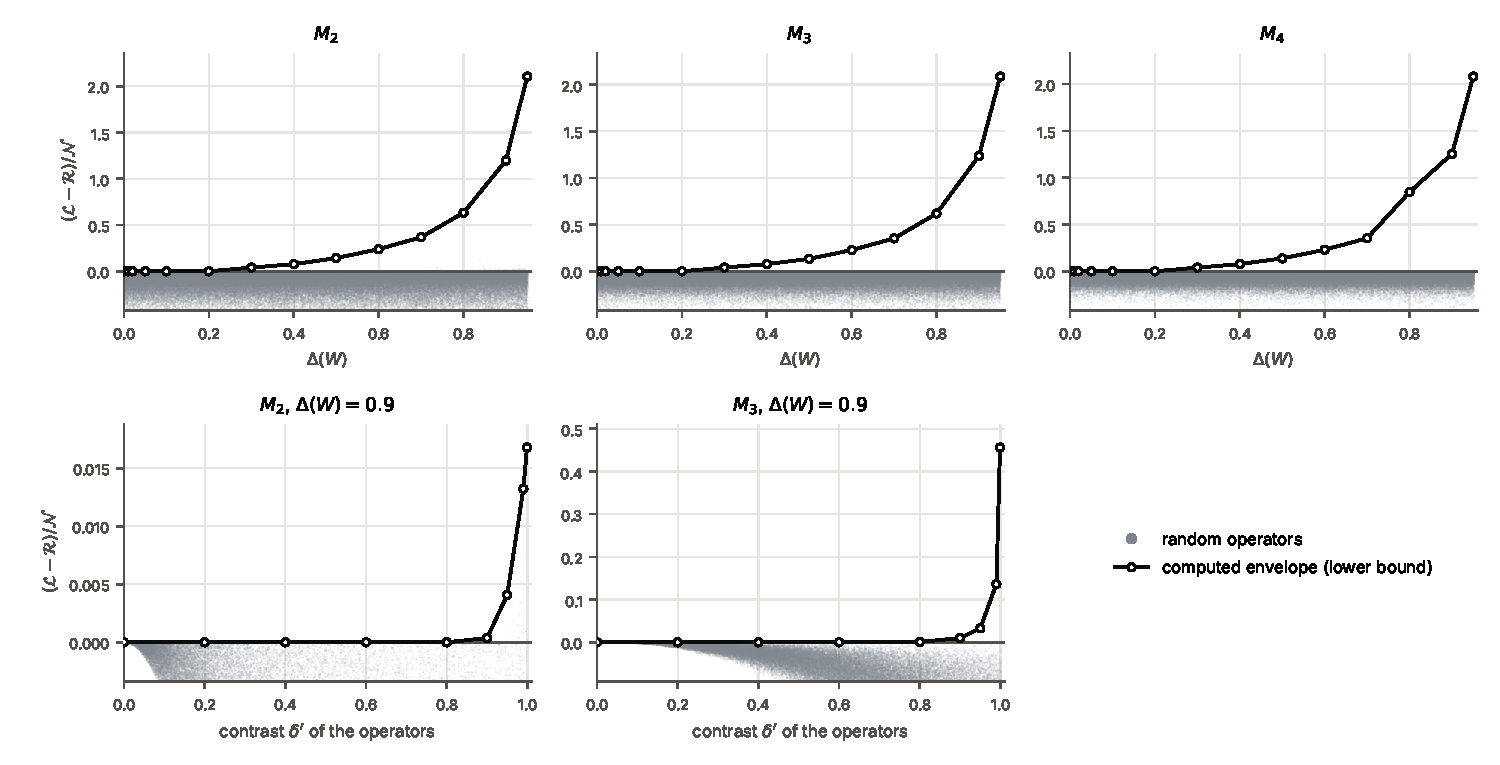
\includegraphics[width=\textwidth]{mc_06_sgm.pdf}
\caption[]{Item 6, $\varphi(A\natural B)\le\sqrt{\varphi(A)\varphi(B)}$: random samples and the computed envelope (a certified lower bound); top: against $\Delta(W)$, bottom: against the contrast $\delta^\prime$ of the operators at $\Delta(W)=0.9$.}
\label{fig:mc-sgm}
\end{figure}

\begin{figure}[!htbp]
\centering
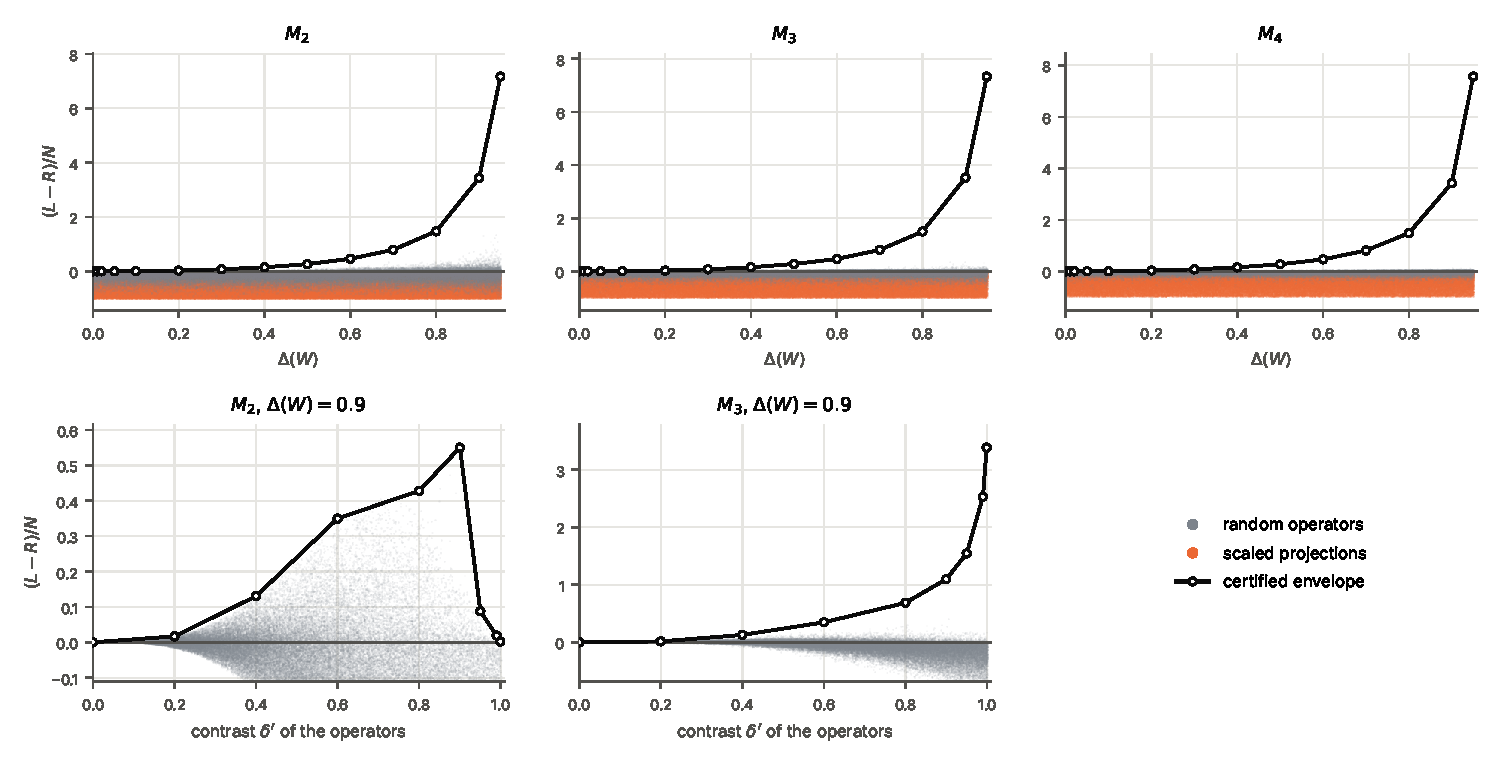
\includegraphics[width=\textwidth]{mc_07_alt.pdf}
\caption[]{Item 7, $\varphi((B^{1/2}AB^{1/2})^2)\le\varphi(BA^2B)$: random samples and the computed envelope (a certified lower bound); top: against $\Delta(W)$, bottom: against the contrast $\delta^\prime$ of the operators at $\Delta(W)=0.9$.}
\label{fig:mc-alt}
\end{figure}

\begin{figure}[!htbp]
\centering
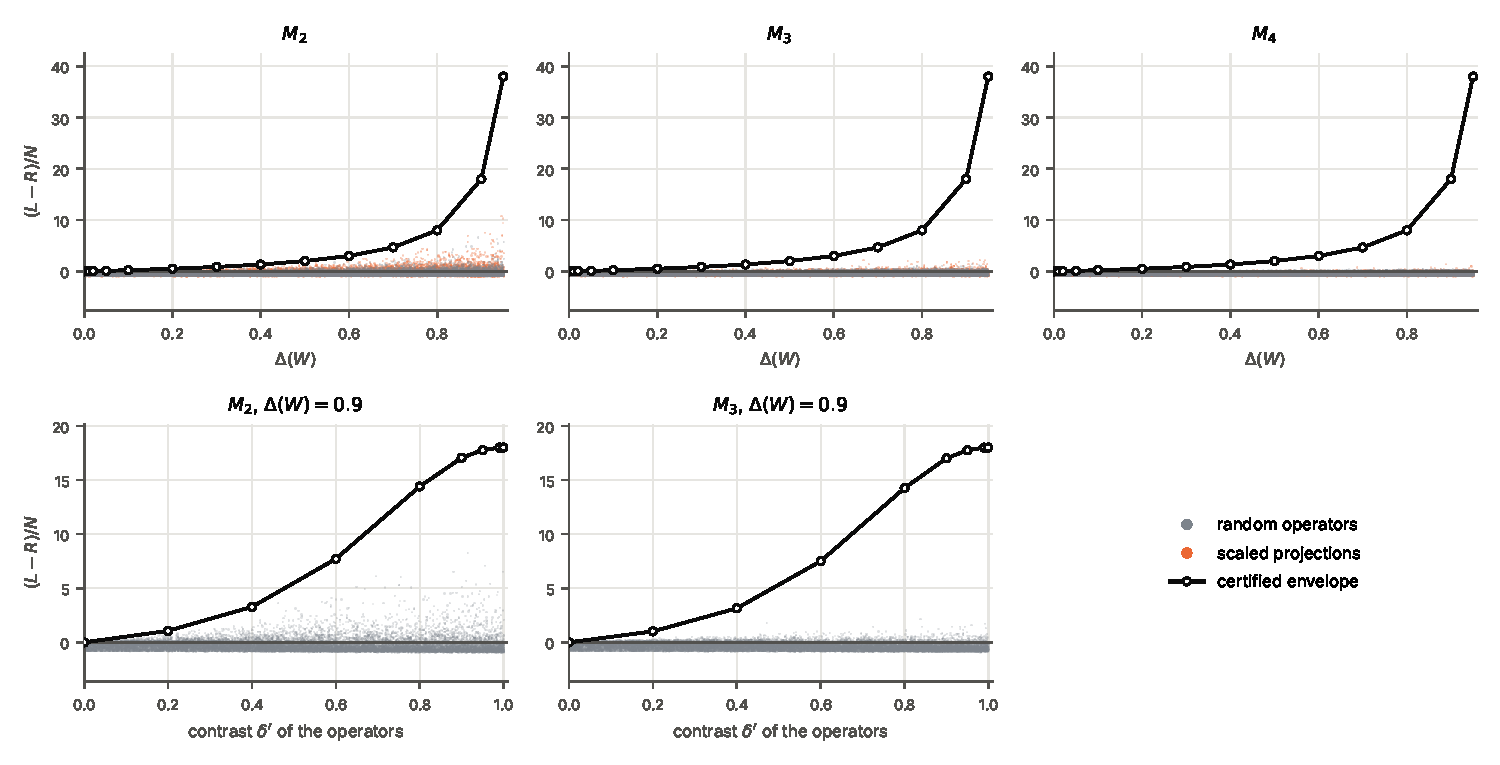
\includegraphics[width=\textwidth]{mc_08_young.pdf}
\caption[]{Item 8, $\varphi(|AB^*|)\le\frac12\varphi(|A|^2)+\frac12\varphi(|B|^2)$: random samples and the computed envelope (a certified lower bound); top: against $\Delta(W)$, bottom: against the contrast $\delta^\prime$ of the operators at $\Delta(W)=0.9$.}
\label{fig:mc-young}
\end{figure}

\begin{figure}[!htbp]
\centering
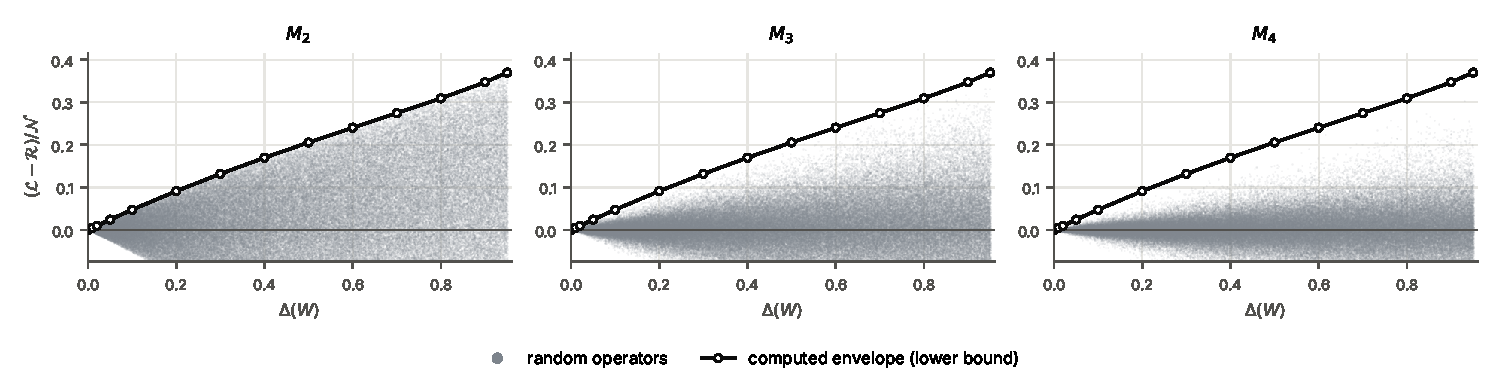
\includegraphics[width=\textwidth]{mc_09_projections.pdf}
\caption[]{Item 9, $\varphi(PQ+QP)\le2\varphi(QPQ)$: random samples and the computed envelope (a certified lower bound) against $\Delta(W)$.}
\label{fig:mc-projections}
\end{figure}

\begin{figure}[!htbp]
\centering
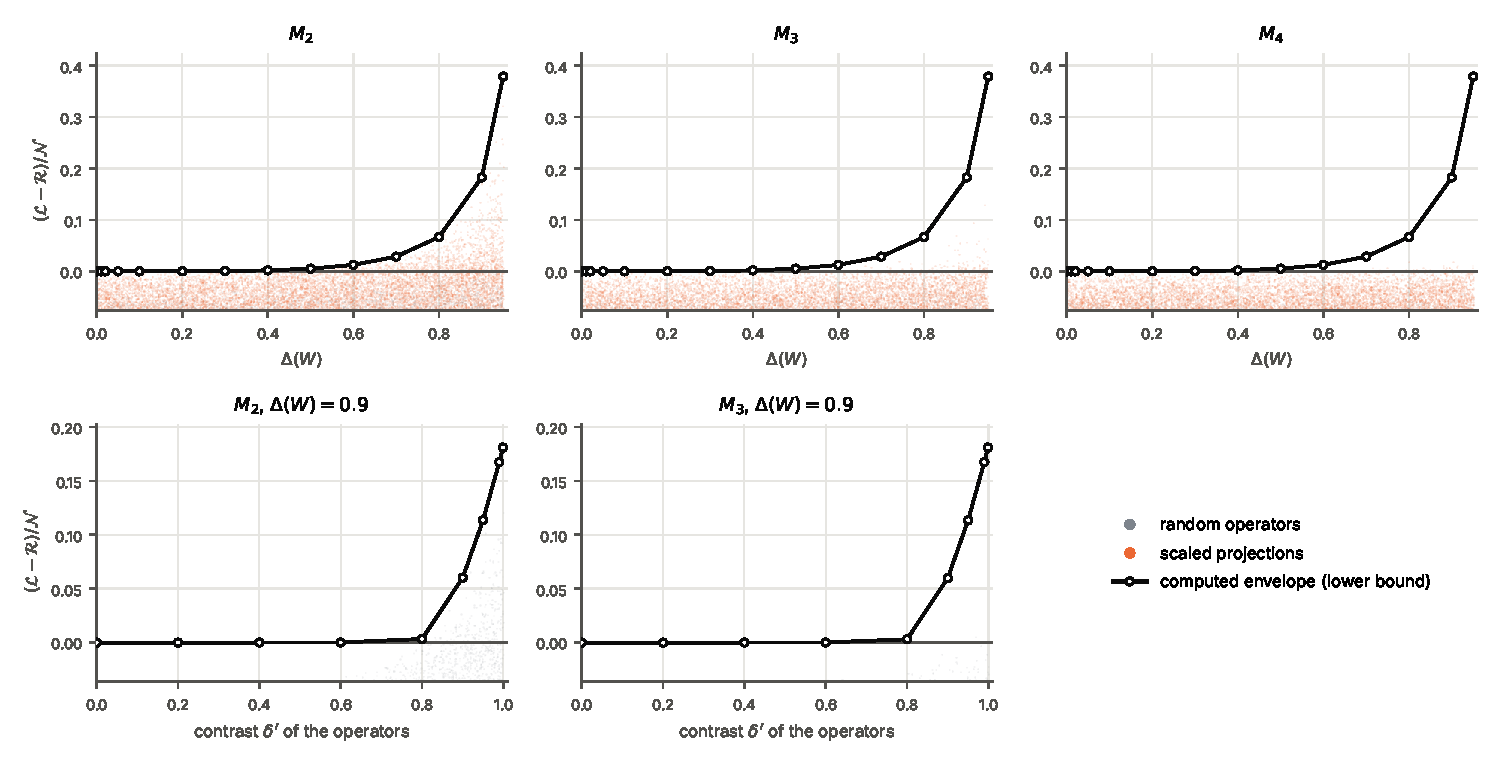
\includegraphics[width=\textwidth]{mc_10_monotone.pdf}
\caption[]{Item 10, $0\le A\le B\Rightarrow\varphi(A^2)\le\varphi(B^2)$: random samples and the computed envelope (a certified lower bound); top: against $\Delta(W)$, bottom: against the contrast $\delta^\prime$ of the operators at $\Delta(W)=0.9$.}
\label{fig:mc-monotone}
\end{figure}

\begin{figure}[!htbp]
\centering
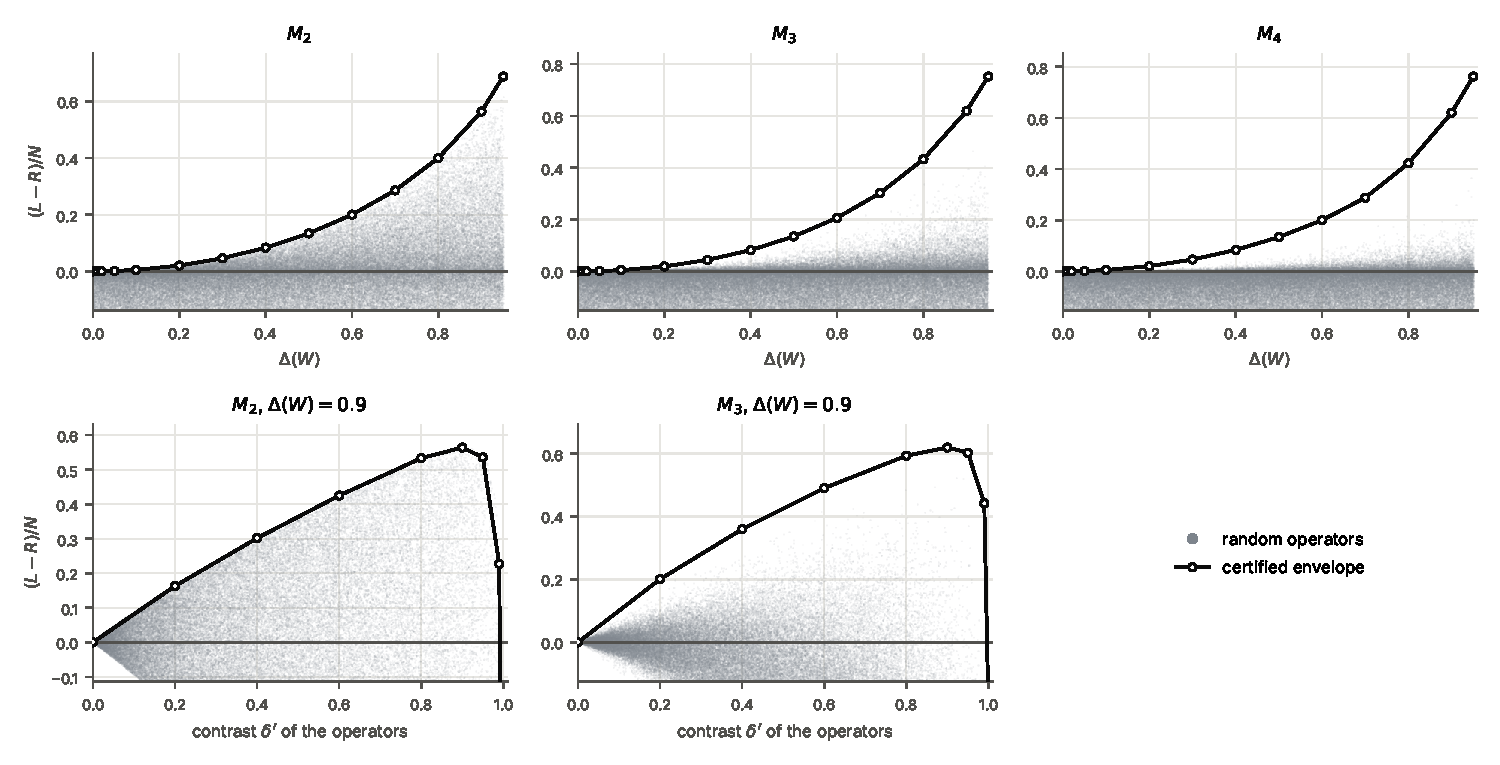
\includegraphics[width=\textwidth]{mc_11_det.pdf}
\caption[]{Item 11, $(\det A)^{1/n}\le\frac1n\varphi(A)$, $\varphi(1)=n$: random samples and the computed envelope (a certified lower bound); top: against $\Delta(W)$, bottom: against the contrast $\delta^\prime$ of the operators at $\Delta(W)=0.9$.}
\label{fig:mc-det}
\end{figure}

\begin{figure}[!htbp]
\centering
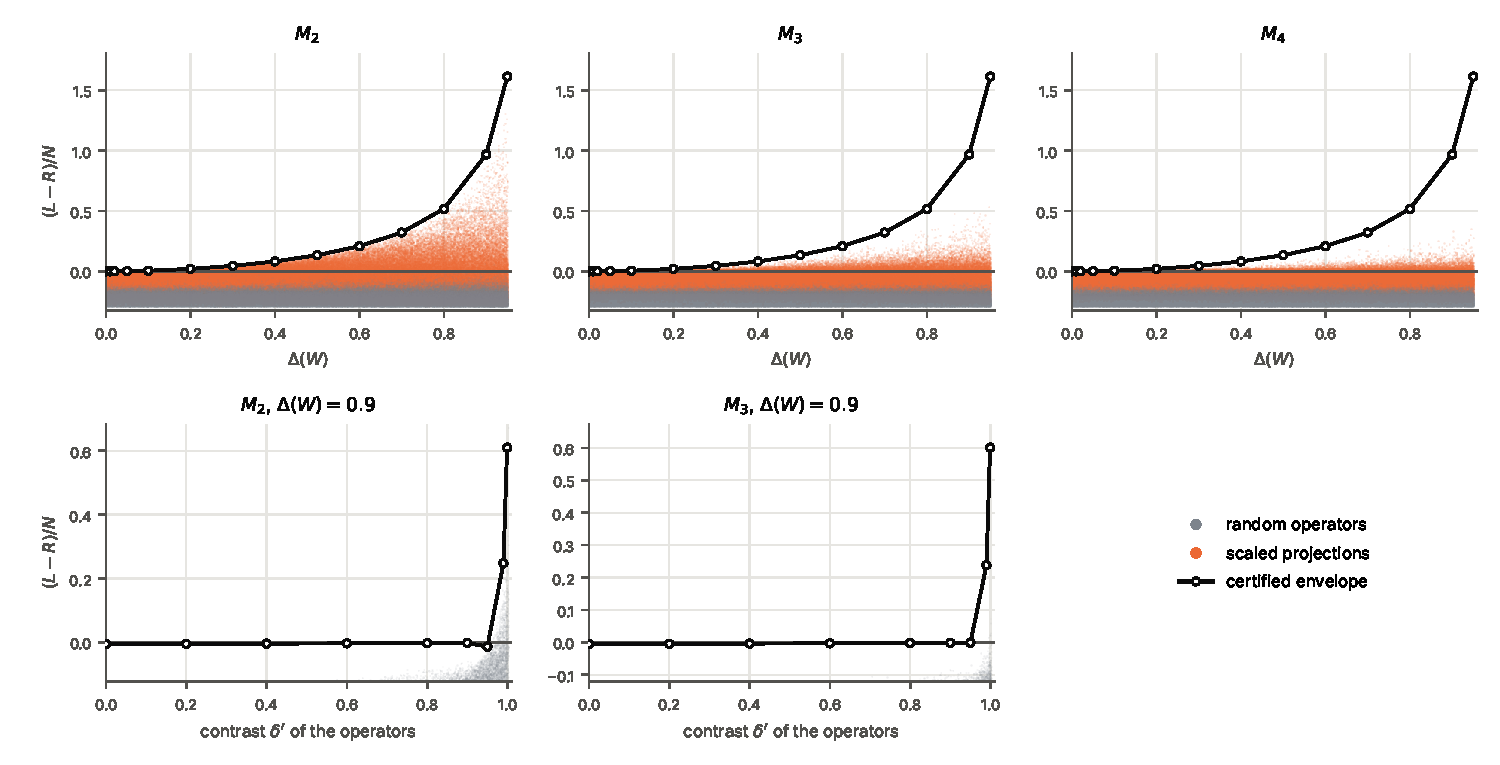
\includegraphics[width=\textwidth]{mc_12_subadd.pdf}
\caption[]{Item 12, $\varphi((A+B)^{1/2})\le\varphi(A^{1/2})+\varphi(B^{1/2})$: random samples and the computed envelope (a certified lower bound); top: against $\Delta(W)$, bottom: against the contrast $\delta^\prime$ of the operators at $\Delta(W)=0.9$.}
\label{fig:mc-subadd}
\end{figure}

\begin{figure}[!htbp]
\centering
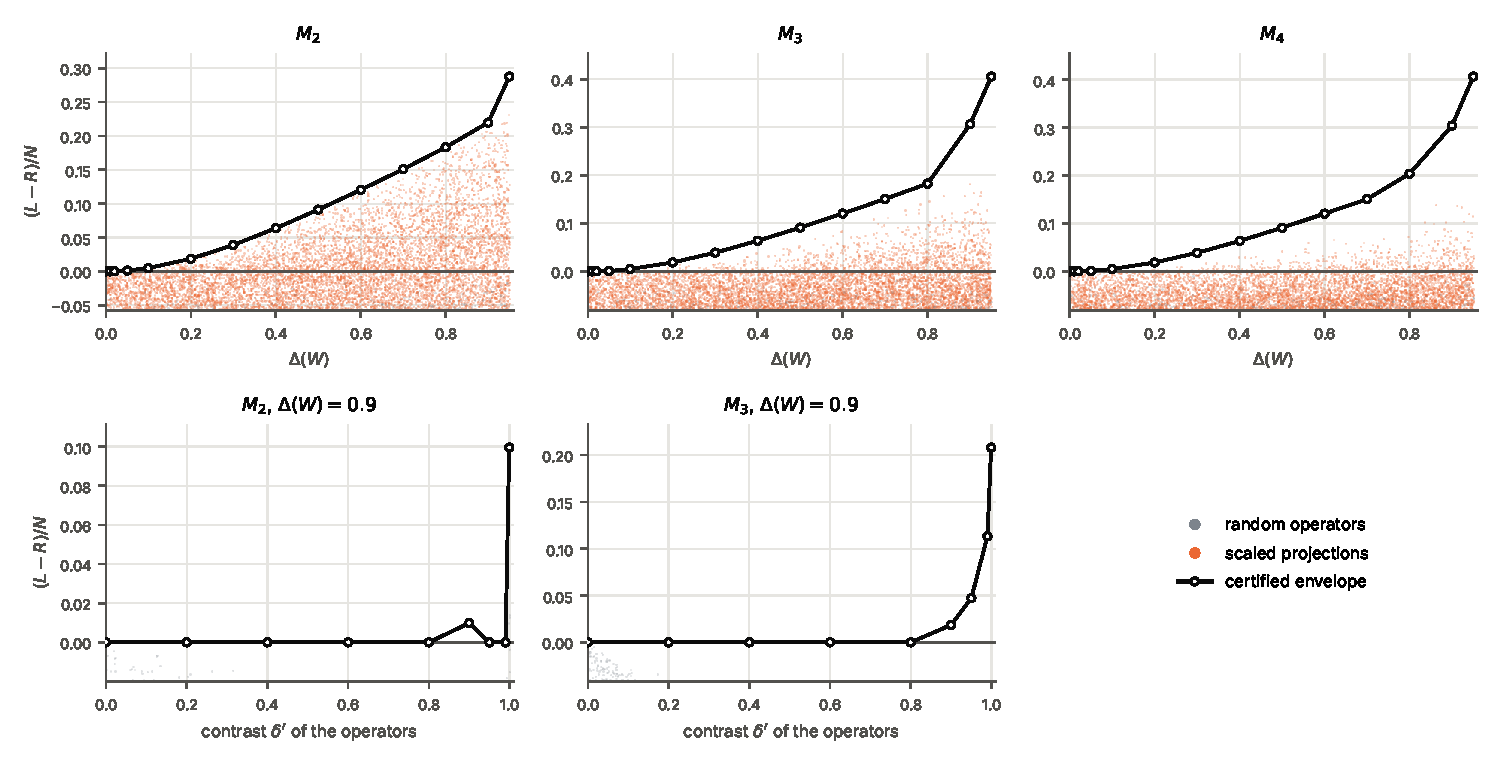
\includegraphics[width=\textwidth]{mc_13_powers.pdf}
\caption[]{Item 13, $\varphi(A+B-|A-B|)\le2\varphi(A^{1/4}B^{1/2}A^{1/4})$: random samples and the computed envelope (a certified lower bound); top: against $\Delta(W)$, bottom: against the contrast $\delta^\prime$ of the operators at $\Delta(W)=0.9$.}
\label{fig:mc-powers}
\end{figure}

\begin{figure}[!htbp]
\centering
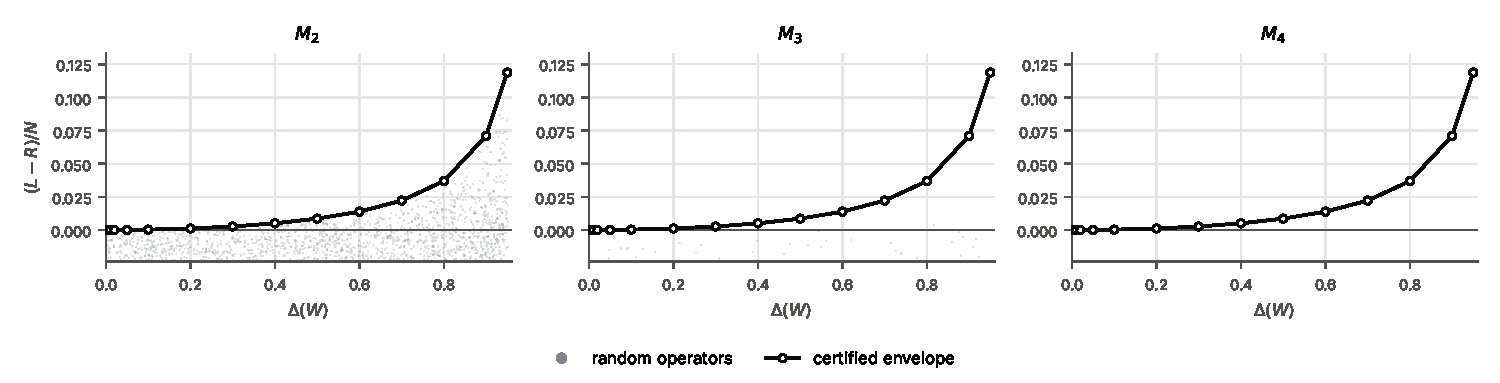
\includegraphics[width=\textwidth]{mc_14_holder.pdf}
\caption[]{Item 14, $|\varphi(PQ)|\le\varphi(P)^{1/3}\varphi(Q)^{2/3}$: random samples and the computed envelope (a certified lower bound) against $\Delta(W)$.}
\label{fig:mc-holder}
\end{figure}

\begin{figure}[!htbp]
\centering
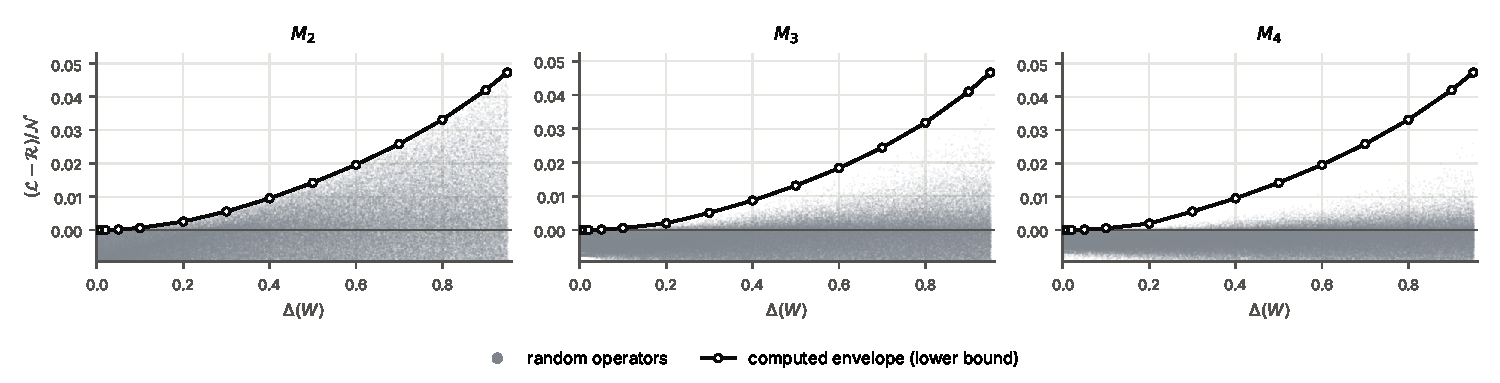
\includegraphics[width=\textwidth]{mc_15_gt.pdf}
\caption[]{Item 15, $\varphi(e^{P+Q})\le\varphi(e^{P/2}e^Qe^{P/2})$: random samples and the computed envelope (a certified lower bound) against $\Delta(W)$.}
\label{fig:mc-gt}
\end{figure}

\begin{figure}[!htbp]
\centering
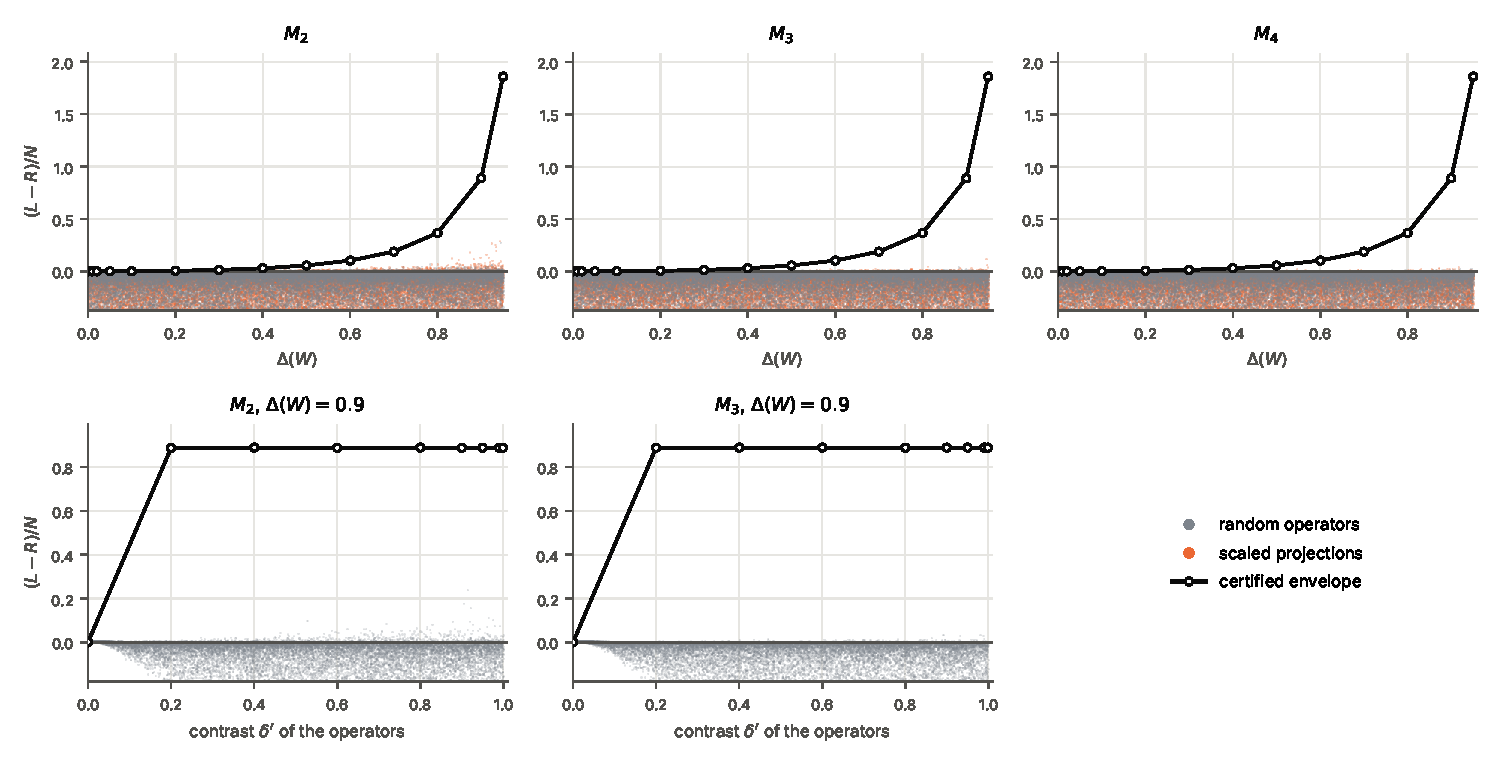
\includegraphics[width=\textwidth]{mc_16_pb.pdf}
\caption[]{Item 16, $\varphi(e^A)e^{\varphi(e^{A/2}Be^{A/2})/\varphi(e^A)}\le\varphi(e^{A+B})$: random samples and the computed envelope (a certified lower bound); top: against $\Delta(W)$, bottom: against the contrast $\delta^\prime$ of the operators at $\Delta(W)=0.9$.}
\label{fig:mc-pb}
\end{figure}

\begin{figure}[!htbp]
\centering
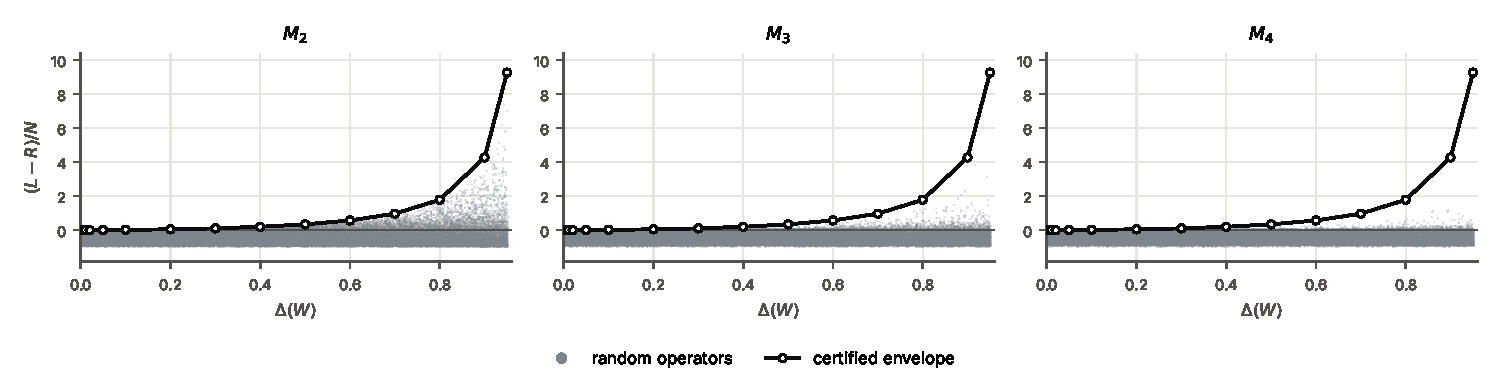
\includegraphics[width=\textwidth]{mc_17_pqp.pdf}
\caption[]{Item 17, $\varphi(PQP)\le\varphi(Q)$: random samples and the computed envelope (a certified lower bound) against $\Delta(W)$.}
\label{fig:mc-pqp}
\end{figure}

\begin{figure}[!htbp]
\centering
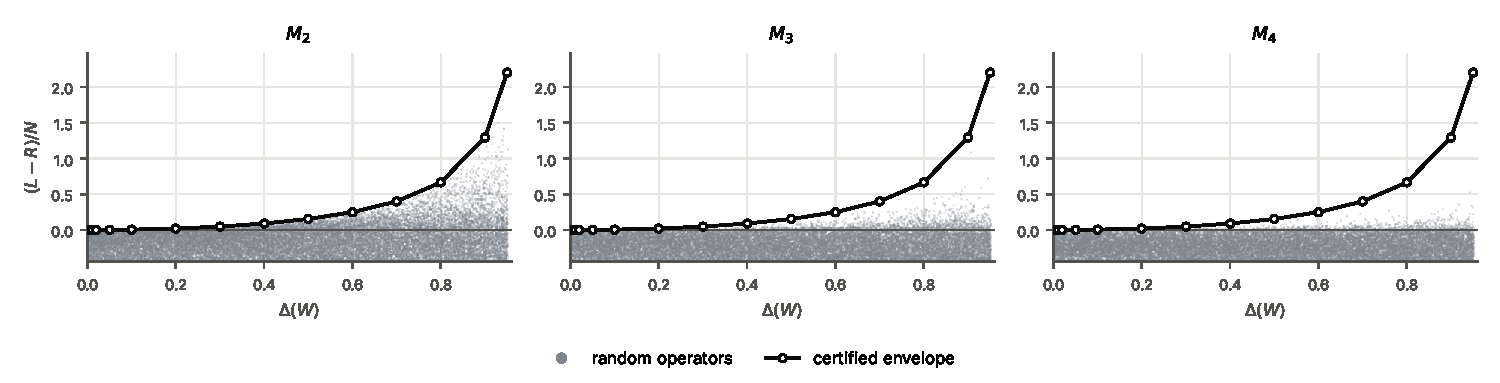
\includegraphics[width=\textwidth]{mc_18_absdiff.pdf}
\caption[]{Item 18, $\varphi(|P-Q|)\le\varphi(P+Q)$: random samples and the computed envelope (a certified lower bound) against $\Delta(W)$.}
\label{fig:mc-absdiff}
\end{figure}

\begin{figure}[!htbp]
\centering
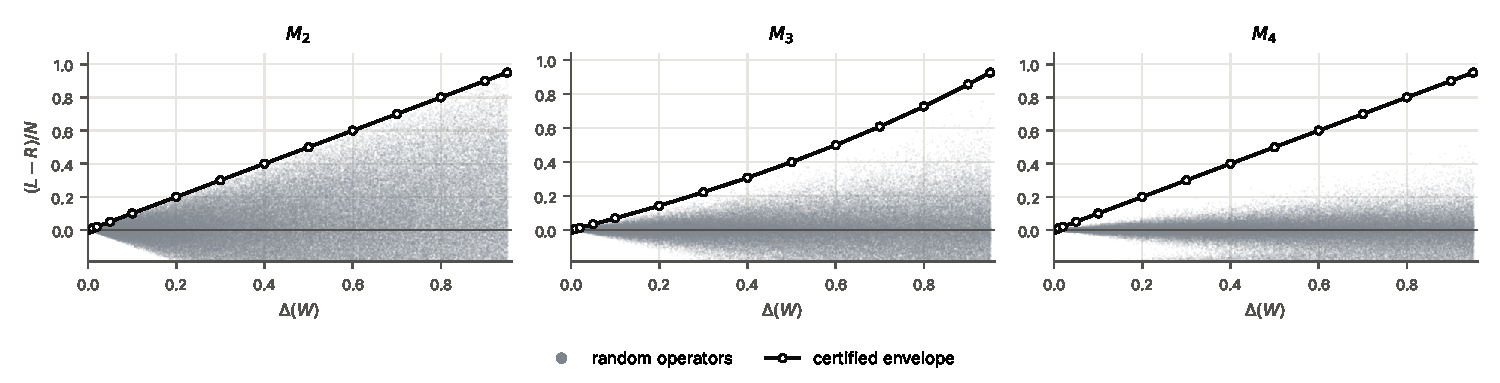
\includegraphics[width=\textwidth]{mc_19_meet.pdf}
\caption[]{Item 19, $\varphi(P+Q)\le\varphi(1+P\wedge Q)$: random samples and the computed envelope (a certified lower bound) against $\Delta(W)$.}
\label{fig:mc-meet}
\end{figure}

\begin{figure}[!htbp]
\centering
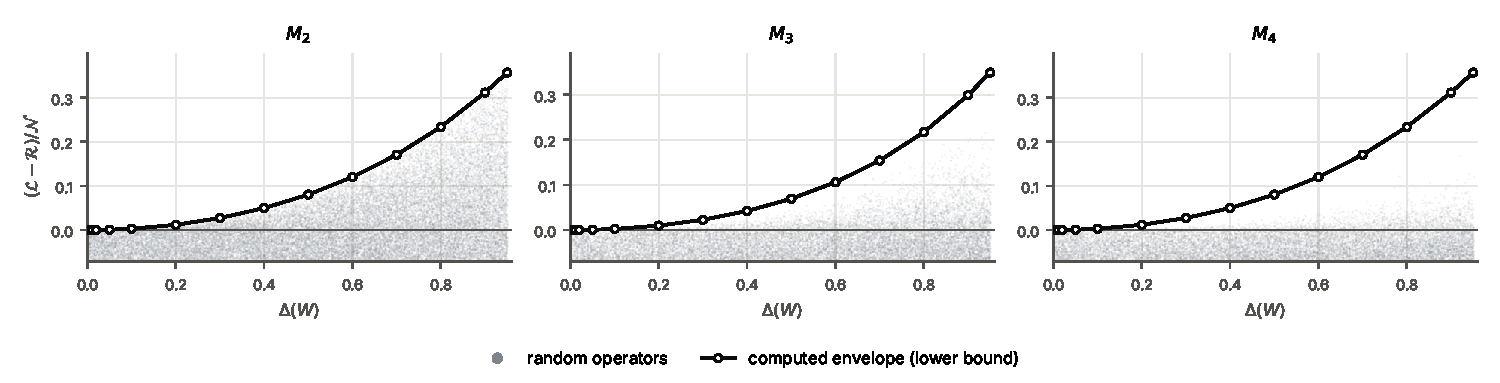
\includegraphics[width=\textwidth]{mc_20_expqpq.pdf}
\caption[]{Item 20, $\varphi(e^{QPQ})\le\varphi(e^P)$: random samples and the computed envelope (a certified lower bound) against $\Delta(W)$.}
\label{fig:mc-expqpq}
\end{figure}

\begin{figure}[!htbp]
\centering
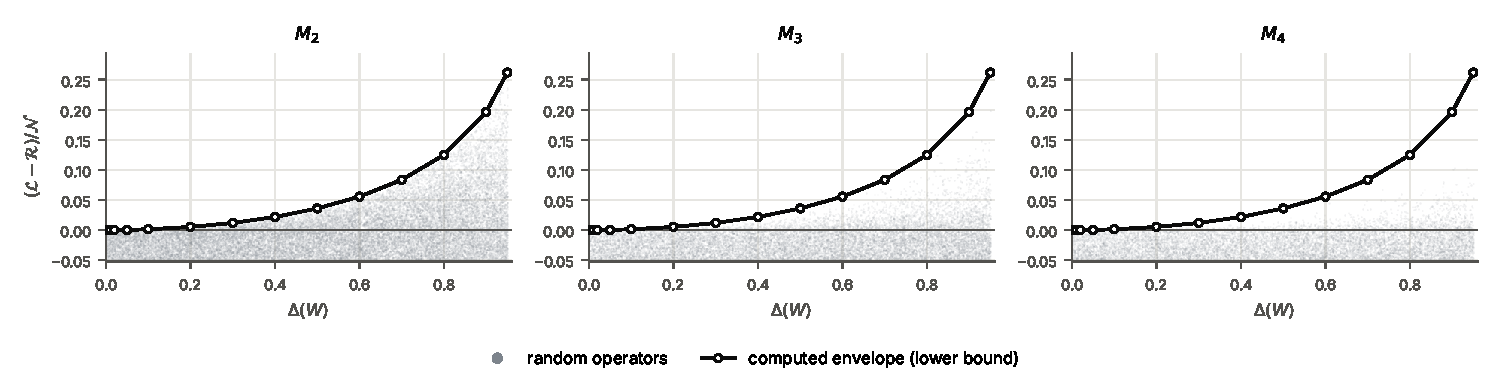
\includegraphics[width=\textwidth]{mc_21_repos.pdf}
\caption[]{Item 21, $\varphi(\mathrm{Re}\,PQ)\ge0$: random samples and the computed envelope (a certified lower bound) against $\Delta(W)$.}
\label{fig:mc-repos}
\end{figure}

\begin{figure}[!htbp]
\centering
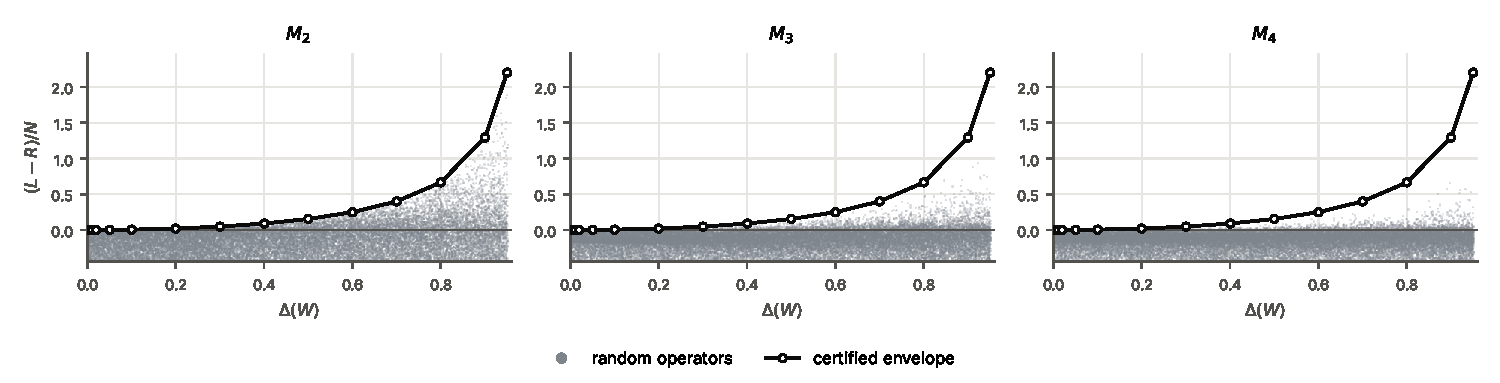
\includegraphics[width=\textwidth]{mc_22_reabs.pdf}
\caption[]{Item 22, $\varphi(\mathrm{Re}\,PQ)\le\varphi(|PQ|)$: random samples and the computed envelope (a certified lower bound) against $\Delta(W)$.}
\label{fig:mc-reabs}
\end{figure}

\begin{figure}[!htbp]
\centering
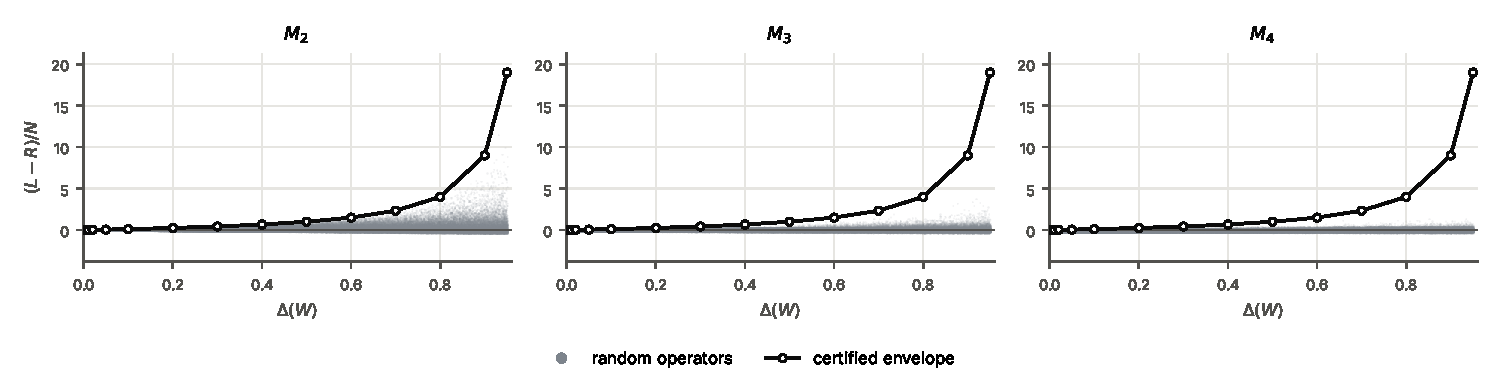
\includegraphics[width=\textwidth]{mc_23_join.pdf}
\caption[]{Item 23, $\varphi(P\vee Q)\le\varphi(P)+\varphi(Q)$: random samples and the computed envelope (a certified lower bound) against $\Delta(W)$.}
\label{fig:mc-join}
\end{figure}

\begin{figure}[!htbp]
\centering
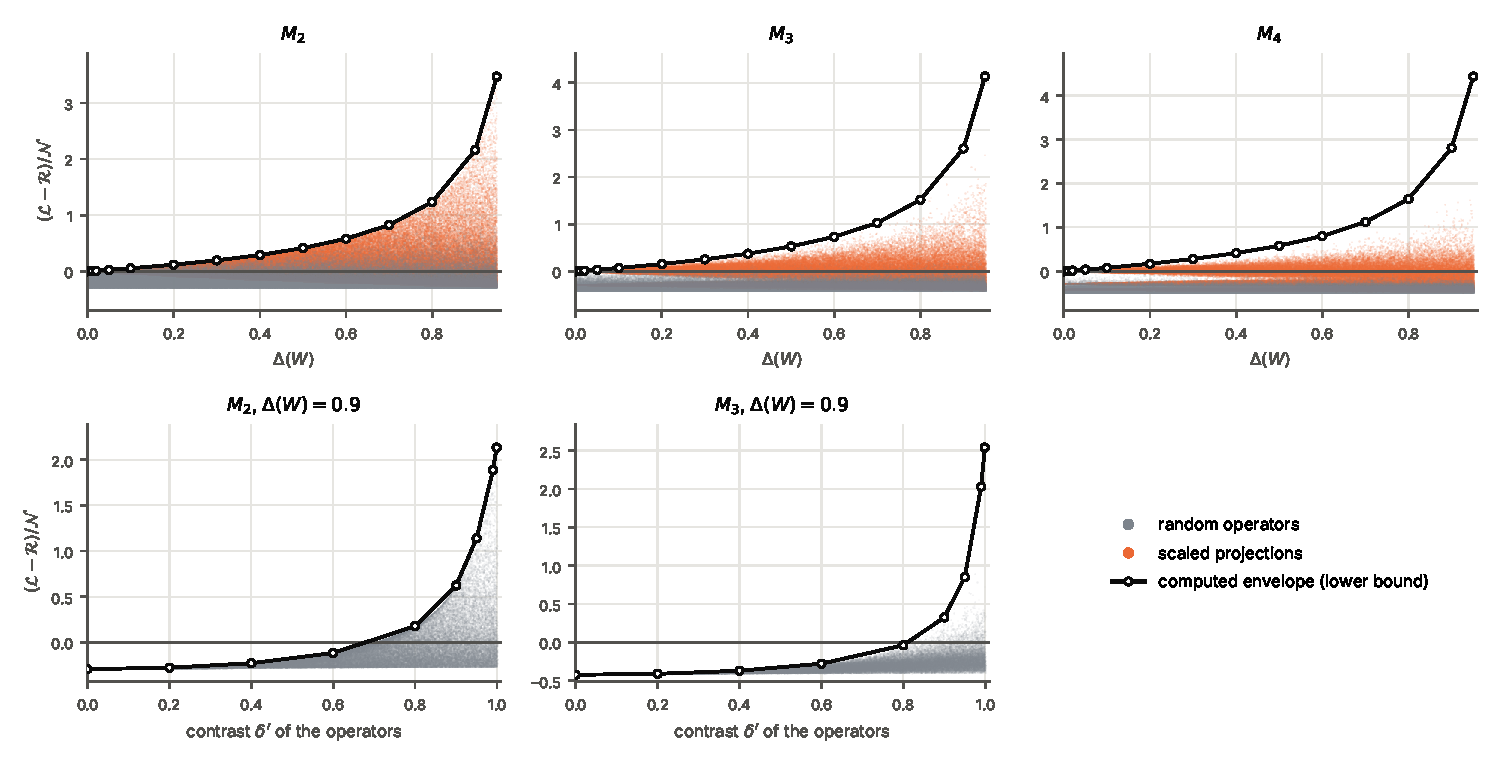
\includegraphics[width=\textwidth]{mc_24_lp.pdf}
\caption[]{Item 24, $\varphi(A^2)^{1/2}\le\varphi(A)$, $\varphi(1)=n$: random samples and the computed envelope (a certified lower bound); top: against $\Delta(W)$, bottom: against the contrast $\delta^\prime$ of the operators at $\Delta(W)=0.9$.}
\label{fig:mc-lp}
\end{figure}

\begin{figure}[!htbp]
\centering
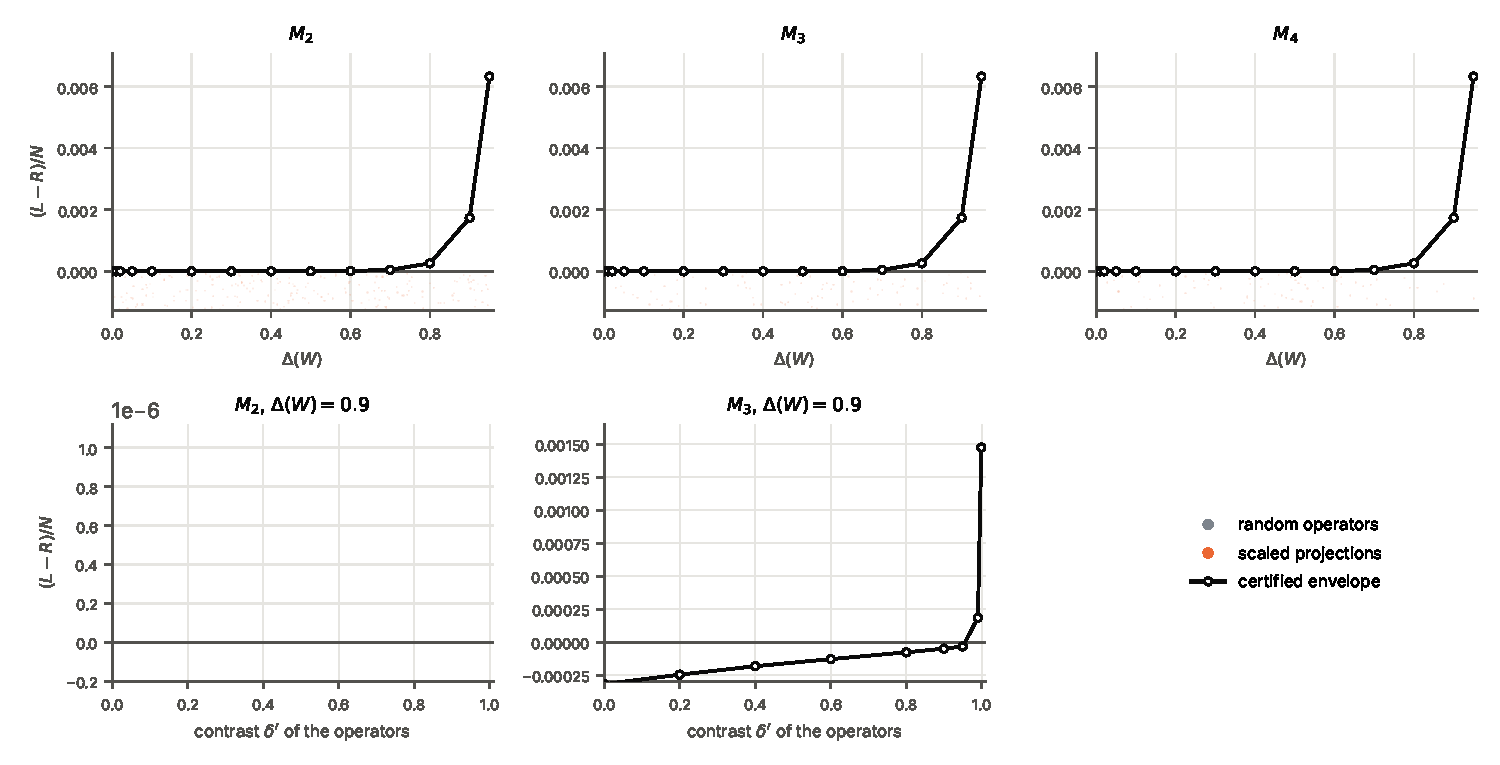
\includegraphics[width=\textwidth]{mc_25_wmon.pdf}
\caption[]{Item 25, $0\le A\le B\Rightarrow\varphi(A^4)\le\varphi(AB^2A)$: random samples and the computed envelope (a certified lower bound); top: against $\Delta(W)$, bottom: against the contrast $\delta^\prime$ of the operators at $\Delta(W)=0.9$.}
\label{fig:mc-wmon}
\end{figure}


\clearpage
{\sloppy
\begin{thebibliography}{99}
\bibitem{abed2024} S.~A.~Abed, I.~A.~Nikolaeva, A.~A.~Novikov, ``Generalisation of Michelson contrast for
  operators and its properties'', Lobachevskii J.\ Math.\ 45 (2024), no.~8, 3835--3848; arXiv:2010.10130.
\bibitem{ando1995} T.~Ando, ``Matrix Young inequalities'', in: \emph{Operator Theory in Function Spaces and Banach
  Lattices}, Oper.\ Theory Adv.\ Appl.\ 75, Birkh\"auser, Basel, 1995, 33--38.
\bibitem{bhatia1997} R.~Bhatia, \emph{Matrix Analysis}, Graduate Texts in Mathematics 169, Springer, 1997.
\bibitem{bikchentaev2005young} A.~M.~Bikchentaev, O.~E.~Tikhonov, ``Characterization of the trace by Young's
  inequality'', J.\ Inequal.\ Pure Appl.\ Math.\ 6 (2005), no.~2, Art.~49.
\bibitem{bikchentaev2007mono} A.~M.~Bikchentaev, O.~E.~Tikhonov, ``Characterization of the trace by monotonicity
  inequalities'', Linear Algebra Appl.\ 422 (2007), no.~1, 274--278.
\bibitem{bikchentaev2009rm} A.~M.~Bikchentaev, ``Commutativity of projectors and trace characterization on von Neumann
  algebras.~I'', Russian Math.\ (Iz.\ VUZ) 53 (2009), no.~12, 68--71.
\bibitem{bikchentaev2010smj} A.~M.~Bikchentaev, ``Commutativity of projections and characterization of traces on von
  Neumann algebras'', Sib.\ Math.\ J.\ 51 (2010), no.~6, 971--977.
\bibitem{bikchentaev2011mn} A.~M.~Bikchentaev, ``Commutation of projections and trace characterization on von
  Neumann algebras.~II'', Math.\ Notes 89 (2011), no.~3--4, 461--471.
\bibitem{bikchentaev2011pb} A.~M.~Bikchentaev, ``The Peierls--Bogoliubov inequality in C$^*$-algebras and
  characterization of tracial functionals'', Lobachevskii J.\ Math.\ 32 (2011), no.~3, 175--179.
\bibitem{bikchentaev2019abed} A.~M.~Bikchentaev, S.~A.~Abed, ``Projections and traces on von Neumann algebras'',
  Lobachevskii J.\ Math.\ 40 (2019), no.~9, 1260--1267.
\bibitem{bikchentaev2019metric} A.~M.~Bikchentaev, ``Metrics on projections of the von Neumann algebra associated
  with tracial functionals'', Sib.\ Math.\ J.\ 60 (2019), 952--956.
\bibitem{bikchentaev2020det} A.~M.~Bikchentaev, ``Inequalities for determinants and characterization of the
  trace'', Sib.\ Math.\ J.\ 61 (2020), no.~2, 248--254.
\bibitem{bikchentaev2025survey} A.~M.~Bikchentaev, M.~S.~Moslehian, ``Characterizations of tracial functionals on
  matrix and operator algebras'', Bull.\ Belg.\ Math.\ Soc.\ Simon Stevin 32 (2025), no.~3, 343--361.
\bibitem{bikchentaev2026moslehian} A.~M.~Bikchentaev, M.~S.~Moslehian, ``Trace inequalities and characterizations
  of tracial functionals in operator algebras'', Positivity 30 (2026), Art.~24; doi:10.1007/s11117-026-01180-0.
\bibitem{bikchentaev2026sgm} A.~M.~Bikchentaev, T.~H.~Dinh, A.~V.~Le, M.~S.~Moslehian, ``Spectral geometric mean
  and trace characterizations'', Positivity 30 (2026), Art.~46.
\bibitem{cho2009} K.~Cho, T.~Sano, ``Young's inequality and trace'', Linear Algebra Appl.\ 431 (2009), no.~8,
  1218--1222.
\bibitem{furuta2005} T.~Furuta, J.~Mi\'ci\'c Hot, J.~Pe\v{c}ari\'c, Y.~Seo, \emph{Mond--Pe\v{c}ari\'c Method in Operator
  Inequalities}, Element, Zagreb, 2005.
\bibitem{gardner1979} L.~T.~Gardner, ``An inequality characterizes the trace'', Canad.\ J.\ Math.\ 31
  (1979), no.~6, 1322--1328.
\bibitem{greub1959} W.~Greub, W.~Rheinboldt, ``On a generalization of an inequality of L.~V.~Kantorovich'', Proc.\
  Amer.\ Math.\ Soc.\ 10 (1959), 407--415.
\bibitem{gustafson1968} K.~Gustafson, ``The angle of an operator and positive operator products'', Bull.\ Amer.\
Math.\ Soc.\ \textbf{74} (1968), 488--492.
\bibitem{gustafsonrao1997} K.~E.~Gustafson, D.~K.~M.~Rao, \emph{Numerical Range: The Field of Values of Linear
Operators and Matrices}, Springer, New York, 1997.
\bibitem{halmos1969} P.~R.~Halmos, ``Two subspaces'', Trans.\ Amer.\ Math.\ Soc.\ 144 (1969), 381--389.
\bibitem{hoa2007} Dinh Trung Hoa, O.~E.~Tikhonov, ``Weighted trace inequalities of monotonicity'', Lobachevskii J.\
  Math.\ 26 (2007), 63--67.
\bibitem{hoa2010} Dinh Trung Hoa, O.~E.~Tikhonov, ``Weighted monotonicity inequalities for traces on operator
  algebras'', Math.\ Notes 88 (2010), no.~1--2, 177--182.
\bibitem{hoa2013} Dinh Trung Hoa, H.~Osaka, Ho Minh Toan, ``On generalized Powers--St{\o}rmer's inequality'', Linear
  Algebra Appl.\ 438 (2013), no.~1, 242--249.
\bibitem{lib} I.~Nikolaeva, A.~Novikov, ``Finite-dimensional Type I von Neumann algebras in PyTorch: a
  GPU-accelerated framework for random block-diagonal operators'', arXiv:2606.15882 (2026);
  code: \url{https://github.com/andre-a-no/von_neumann_type_i}.
\bibitem{moslehian2025jmaa} M.~S.~Moslehian, A.~M.~Bikchentaev, ``Characterizations of the canonical trace on full
  matrix algebras'', J.\ Math.\ Anal.\ Appl.\ 552 (2025), no.~2, 129764.
\bibitem{novikov2015} A.~A.~Novikov, O.~E.~Tikhonov, ``Characterization of central elements of operator
  algebras by inequalities'', Lobachevskii J.\ Math.\ 36 (2015), no.~2, 208--210.
\bibitem{petz1988} D.~Petz, J.~Zem\'anek, ``Characterizations of the trace'', Linear Algebra Appl.\ 111
  (1988), 43--52.
\bibitem{sano2006} T.~Sano, T.~Yatsu, ``Characterizations of tracial property via inequalities'', J.\ Inequal.\ Pure
  Appl.\ Math.\ 7 (2006), no.~1, Art.~36.
\bibitem{specht1960} W.~Specht, ``Zur Theorie der elementaren Mittel'', Math.\ Z.\ 74 (1960), 91--98.
\bibitem{stolyarov2002} A.~I.~Stolyarov, O.~E.~Tikhonov, A.~N.~Sherstnev, ``Characterization of normal traces on
  von Neumann algebras by inequalities for the modulus'', Math.\ Notes 72 (2002), no.~3--4, 411--416.
\bibitem{strang1962} W.~G.~Strang, ``Eigenvalues of Jordan products'', Amer.\ Math.\ Monthly \textbf{69} (1962),
37--40.
\bibitem{tikhonov2005} O.~E.~Tikhonov, ``Subadditivity inequalities in von Neumann algebras and characterization of
  tracial functionals'', Positivity 9 (2005), no.~2, 259--264.
\end{thebibliography}
}

\end{document}
